% This is part of Mes notes de mathématique
% Copyright (c) 2006-2021
%   Laurent Claessens, Carlotta Donadello
% See the file fdl-1.3.txt for copying conditions.

%+++++++++++++++++++++++++++++++++++++++++++++++++++++++++++++++++++++++++++++++++++++++++++++++++++++++++++++++++++++++++++
\section{Limite de fonctions}
%+++++++++++++++++++++++++++++++++++++++++++++++++++++++++++++++++++++++++++++++++++++++++++++++++++++++++++++++++++++++++++

%---------------------------------------------------------------------------------------------------------------------------
\subsection{Définition}
%---------------------------------------------------------------------------------------------------------------------------

La définition générale de la limite est~\ref{DefYNVoWBx}. Dans le cas de fonctions \( \eR\to \eR\), elle peut s'écrire de façon plus efficace. La proposition suivante montre comment fonctionne la limite pour une fonction définie sur tout \( \eR\).

\begin{proposition}[Caractérisation de la limite]       \label{PropAJQQooQQClfp}
	Soit une fonction $f\colon \eR\to \eR$ définie sur \( \eR\) et $a\in \eR$. La fonction \( f\) admet la limite \( \ell\) pour \( x\to a\) si et seulement si il existe un réel $\ell$ tel que pour tout \( \epsilon>0\), il existe un \( \delta>0\) tel que
	\begin{equation}\label{EqDefLimiteFonction}
		0<| x-a |<\delta\Rightarrow| f(x)-\ell |<\varepsilon.
	\end{equation}
\end{proposition}

\begin{proof}
    Il s'agit de montrer l'équivalence avec la définition~\ref{DefYNVoWBx}. Nous allons faire un usage intensif de la remarque~\ref{RemQDRooKnwKk}\ref{ITEMooUIHJooXAFaJa}.
    \begin{subproof}
    \item[Sens direct]
        Soient \( \epsilon>0\) et \( V=B(\ell,\epsilon)\). Alors il existe un voisinage \( W\) de \( a\) dans \( \eR\) tel que
        \begin{equation}
            f\big( W\setminus\{ a \} \big)\subset V.
        \end{equation}
        Soit \( \delta\) tel que \( B(a,\delta)\subset W\). Nous avons encore
        \begin{equation}
            f\big( B(a,\delta)\setminus\{ a \} \big)\subset V.
        \end{equation}
        Soit maintenant \( x\in \eR\) tel que $0<| x-a |<\delta$. Cela signifie \( x\in B(a,\delta)\setminus\{ a \}\). Pour un tel \( x\) nous avons donc \( f(x)\in B(\ell,\epsilon)\), c'est-à-dire \( | f(x)-\ell |<\epsilon\).
    \item[Dans l'autre sens]
        Soient un voisinage \( V\) de \( \ell\) et \( \epsilon>0\) tel que \( B(\ell,\epsilon)\subset V\). Nous considérons \( \delta\) tel que \( 0<| x-a |<\delta\) implique \( | f(x)-\ell |<\epsilon\).

        Avec tout cela nous posons \( W=B(x,\delta)\), et nous avons
        \begin{equation}
            f\big( W\setminus\{ a \} \big)\subset B(\ell,\alpha)\subset V.
        \end{equation}
    \end{subproof}
\end{proof}

Si aucun nombre $\ell$ ne vérifie la condition de la définition, alors on dit que la fonction n'admet pas de limite en $a$. Lorsque $f$ possède la limite $\ell$ en $a$, nous notons
\begin{equation}
	\lim_{x\to a} f(x)=\ell.
\end{equation}

La proposition suivante a déjà été démontrée dans la proposition~\ref{PropFObayrf}. Nous en donnons ici une démonstration adaptée au cas \( \eR\to \eR\).

\begin{proposition}
	Soit une fonction $f\colon D\to \eR$. Si $a$ est un point d'accumulation de $D$ et s'il existe une limite de $f$ en $a$, alors il en existe une seule.
\end{proposition}


\begin{proof}
    Nous prouvons qu'il ne peut pas exister deux nombres $\ell\neq\ell'$ vérifiant tout les deux la condition \eqref{EqDefLimiteFonction}.

	Soient $\ell$ et $\ell'$ deux limites de $f$ au point $a$. Par définition, pour tout $\varepsilon$ nous avons des nombres $\delta$ et $\delta'$ tels que
	\begin{equation}	\label{EqsContf2307Right}
		\begin{aligned}[]
			| x-a |<\delta&\Rightarrow \big| f(x)-\ell \big|<\varepsilon\\
			| x-a |<\delta'&\Rightarrow \big| f(x)-\ell' \big|<\varepsilon
		\end{aligned}
	\end{equation}
	Pour fixer les idées, supposons que $\delta<\delta'$ (le cas $\delta\geq\delta'$ se traite de la même manière).

	Étant donné que $a$ est un point d'accumulation du domaine $D$ de $f$, il existe un $x\in D$ tel que $| x-a |<\delta$. Évidemment, nous avons aussi $| x-a |<\delta'$. Les conditions \eqref{EqsContf2307Right} signifient alors que ce $x$ vérifie en même temps
	\begin{equation}
		| f(x)-\ell |<\varepsilon,
	\end{equation}
	et
	\begin{equation}
		| f(x)-\ell' |<\varepsilon.
	\end{equation}
	Afin de prouver que $\ell=\ell'$, nous allons maintenant calculer $| \ell-\ell' |$ et montrer que cette distance est plus petite que tout nombre. Nous avons (voir remarque~\ref{RemTechniqueIneqs})
	\begin{equation}	\label{EqInesq2307ellellepr}
		| \ell-\ell' |=| \ell-f(x)+f(x)-\ell' |\leq | \ell-f(x) |+| f(x)-\ell' |<\varepsilon+\varepsilon.
	\end{equation}
	En résumé, pour tout $\varepsilon>0$ nous avons
	\begin{equation}
		| \ell-\ell' |<2\varepsilon,
	\end{equation}
	et donc $| \ell-\ell' |=0$, ce qui signifie que $\ell=\ell'$.
\end{proof}

\begin{remark}		\label{RemTechniqueIneqs}
	Les inégalités \eqref{EqInesq2307ellellepr} utilisent deux techniques très classiques en analyse qu'il convient d'avoir bien compris. La première est de faire
	\begin{equation}
		| A-B |=| A-C+C-B |.
	\end{equation}
	Il s'agit d'ajouter $-C+C$ dans la norme. Évidemment, cela ne change rien.

	La seconde technique est l'inégalité
	\begin{equation}
		| A+B |\leq| A |+| B |.
	\end{equation}
\end{remark}

\begin{example}
	Considérons la fonction $f(x)=2x$, et calculons la limite $\lim_{x\to 3} f(x)$. Vu que $f(3)=6$, nous nous attendons à avoir $\ell=6$. C'est ce que nous allons prouver maintenant. Pour chaque $\varepsilon>0$ nous devons trouver un $\delta>0$ tel que $| x-3 |<\delta$ implique $| f(x)-6 |<\varepsilon$. En remplaçant $f(x)$ par sa valeur en fonction de $x$ et avec quelques manipulations nous trouvons :
	\begin{equation}
		\begin{aligned}[]
			| f(x)-6 |&<\varepsilon\\
			| 2x-6 |&<\varepsilon\\
			2| x-3 |&<\varepsilon\\
			| x-3 |&<\frac{ \varepsilon }{2}
		\end{aligned}
	\end{equation}
	Donc dès que $| x-3 |<\frac{ \varepsilon }{2}$, nous avons $| f(x)-6 |<\varepsilon$. Nous posons donc $\delta=\frac{ \varepsilon }{2}$.

	Plus généralement, nous avons $\lim_{x\to a} f(x)=2a$, et cela se prouve en étudiant $| f(x)-2a |$ exactement de la même manière.
\end{example}

%---------------------------------------------------------------------------------------------------------------------------
\subsection{Quelques règles de calcul}
%---------------------------------------------------------------------------------------------------------------------------


En plus d'être linéaire, la limite possède les deux propriétés suivantes.
\begin{proposition}     \label{PROPooDQFIooMMwxxJ}
	Si $f$ et $g$ sont deux fonctions qui admettent une limite en $a$, alors
	\begin{equation}
		\lim_{x\to a} (fg)(x)=\lim_{x\to a} f(x)\cdot\lim_{x\to a} g(x).
	\end{equation}
	Si de plus $\lim_{x\to a} g(x)\neq 0$, alors
	\begin{equation}
		\lim_{x\to a} \frac{ f(x) }{ g(x) }=\frac{ \lim_{x\to a} f(x) }{ \lim_{x\to a} g(x) }.
	\end{equation}
\end{proposition}

\begin{theorem}     \label{ThoLimLinMul}
    Si
    \begin{equation} \label{Eqhypmullimlin}
      \lim_{x\to a}f(x)=b,
    \end{equation}
    alors
    \begin{equation} \label{Eqbutmultlim}
      \lim_{x\to a}(\lambda f)(x)=\lambda b
    \end{equation}
    pour n'importe quel $\lambda\in\eR$.
\end{theorem}

\begin{proof}
Soit $\epsilon>0$. Afin de prouver la propriété \eqref{Eqbutmultlim}, il faut trouver un $\delta$ tel que pour tout $x$ dans $[a-\delta,a+\delta]$, on ait $| (\lambda f)(x)- \lambda b |\leq\epsilon$. Cette dernière inégalité est équivalente à $|\lambda|| f(x)-b |\leq\epsilon$. Nous devons donc trouver un $\delta$ tel que
\begin{equation}
| f(x)-b |\leq\frac{ \epsilon }{ | \lambda | }.
\end{equation}
soit vraie pour tout $x$ dans $[a-\delta,a+\delta]$. Mais l'hypothèse \eqref{Eqhypmullimlin} dit précisément qu'il existe un $\delta$ tel que pour tout $x$ dans $[a-\delta,a+\delta]$ on ait cette inégalité.
\end{proof}

\begin{theorem}     \label{ThoLimLin}
    Si
    \begin{subequations}
    \begin{align}
        \lim_{x\to a}f(x)&=b_1\\
        \lim_{x\to a}g(x)&=b_2,
    \end{align}
    \end{subequations}
    alors
    \begin{equation}
        \lim_{x\to a}(f+g)(x)=b_1+b_2.
    \end{equation}
\end{theorem}

\begin{proof}
    Soit $\epsilon>0$. Par hypothèse, il existe $\delta_1$ tel que
    \begin{equation}    \label{Eqfbunepsdeux}
      | f(x)-b_1 |\leq \frac{ \epsilon }{ 2 }
    \end{equation}
    dès que $| x-a |\leq\delta_1$. Il existe aussi $\delta_2$ tel que
    \begin{equation}    \label{Eqgbdeuxepsdeux}
      | g(x)-b_2 |\leq \frac{ \epsilon }{ 2 }.
    \end{equation}
    dès que $| x-a |\leq \delta_2$. Tu notes l'astuce de prendre $\epsilon/2$ dans la définition de limite pour $f$ et $g$. Maintenant, ce qu'on voudrait c'est un $\delta$ tel que l'on ait $| (f+g)(x)-(b_1+b_2) |\leq \epsilon$ dès que $| x-a |\leq \delta$. Moi je dit que $\delta=\min\{ \delta_1,\delta_2 \}$ fonctionne. En effet, en utilisant l'inégalité $| a+b |\leq | a |+| b |$, nous trouvons :
    \begin{align}
    | (f+g)(x)-(b_1+b_2) |=| (f(x)-b_1)+(g(x)-b_2) |
            \leq | f(x)-b_1 |+| g(x)-b_2 |.     \label{Eqfplusgfbun}
    \end{align}
    Comme on suppose que $| x-a |\leq\delta$, on a évidemment $| x-a |\leq\delta_1$, et donc l'équation \eqref{Eqfbunepsdeux} tient. Mais si $| x-a |\leq\delta$, on a aussi $| x-a |\leq\delta_2$, et donc l'équation  \eqref{Eqfbunepsdeux} tient également. Chacun des deux termes de \eqref{Eqfplusgfbun} est donc plus petits que $\epsilon/2$, et donc le tout est plus petit que $\epsilon$, ce qu'il fallait montrer.
\end{proof}

\begin{proposition}     \label{PROPooVLBWooVttvFK}
    La limite est linéaire : pour pour toutes fonctions $f$ et $g$ admettant une limite en $a$ et pour tout réels $\lambda$ et $\mu$.
    \begin{equation}
        \lim_{x\to a} (\lambda f+\mu g)(x)=\lambda\lim_{x\to a} f(x)+\mu\lim_{x\to a} g(x).
    \end{equation}
\end{proposition}

\begin{proof}
    Il s'agit seulement des deux propriétés des théorèmes \ref{ThoLimLinMul} et \ref{ThoLimLin}.
\end{proof}

\begin{lemma}       \label{LEMooYJGLooVBaglB}
    Soient un espace vectoriel normé \( V\) ainsi qu'une fonction \( f\colon \eR\to V\) telle que \( \lim_{t\to 0} f(t)=v\). Alors pour tout \( \lambda\in \eR\) nous avons
    \begin{equation}
        \lim_{t\to 0} f(\lambda t)=v.
    \end{equation}
\end{lemma}

\begin{proof}
    Nous utilisons la caractérisation \eqref{PropAJQQooQQClfp} de la limite. Soit \( \epsilon>0\). Soit \( \delta>0\) tel que \( \| f(t)-v \|<\epsilon\) pour tout \( | t |<\delta\). Nous considérons alors \( \delta'=\delta/| \lambda |\).

    Si \( | t |<\delta'\), alors \( | \lambda t |<\delta\) et nous avons bien \( \| f(\lambda t)-v \|<\epsilon\).
\end{proof}

\begin{proposition}[\cite{TrenchRealAnalisys}]      \label{PROPooOUPNooTrClHw}
    Soient des fonctions \( f,g\colon \eR\to \eR\) telles que \( \lim_{x\to a} f(x)=\ell\) et \( \lim_{x\to a} g(x)=\ell'\neq 0\). Alors
    \begin{equation}
        \lim_{x\to a} \frac{ f(x) }{ g(x) }=\frac{ \ell }{ \ell' }.
    \end{equation}
\end{proposition}

\begin{proof}
    Nous avons :
    \begin{equation}
        \left| \frac{ f(x) }{ g(x) }-\frac{ \ell }{ \ell' } \right| =\frac{ | \ell'f(x)-g(x)\ell | }{ |g(x)\ell| }.
    \end{equation}
    Soit \( s\), un minorant de \( | g(x) |\) sur un voisinage de \( a\); vu que la limite en \( a\) est \( \ell'\neq 0\), nous pouvons prendre par exemple \( s=\ell'/2\) : \( | g(x) |>\ell'/2\) sur \( B(a,\delta)\) dès que \( \delta\) est assez petit. Nous considérons \( x\in B(a,\delta)\). Avec cela nous avons :
    \begin{subequations}
        \begin{align}
            \left| \frac{ f(x) }{ g(x) }-\frac{ \ell }{ \ell' } \right| &=\frac{ | \ell'f(x)-g(x)\ell | }{ |g(x)\ell| }\\
            &\leq \frac{ 2 }{ | \ell'} |\left( \frac{ | \ell'f(x)-g(x)\ell | }{ | \ell' | } \right) \\
            &\leq \frac{ 2 }{ | \ell' |^2 }\big( | \ell'f(x)-\ell\ell' |+| \ell\ell'-g(x)\ell | \big)\\
            &=\frac{ 2 }{ | \ell' |^2 }\big( | \ell' | |f(x)-\ell |+| \ell | |\ell'-g(x) | \big).
        \end{align}
    \end{subequations}
    Soient \( \epsilon>0\) et \( \delta\) tel que \( | f(x)-\ell |<\epsilon\) et \( | g(x)-\ell' |<\epsilon\) pour tout \( x\in B(a,\delta)\). Avec cela nous avons
    \begin{equation}
        \left| \frac{ f(x) }{ g(x) }-\frac{ \ell }{ \ell' } \right| \leq\frac{ 2 }{ | \ell' |^2\big( | \ell' |+| \ell | \big) }\epsilon.
    \end{equation}
    D'où la limite attendue.
\end{proof}

\begin{lemma}       \label{LemLimMajorableVois}
    Si $\lim_{x\to a}f(x)=b$ avec $a$, $b\in\eR$, alors il existe un $\delta>0$ et un $M>0$ tels que
    \[
        (| x-a |\leq\delta)\Rightarrow | f(x) |\leq M.
    \]
\end{lemma}

Ce que signifie ce lemme, c'est que quand la fonction $f$ admet une limite finie en un point, alors il est possible de majorer la fonction sur un intervalle autour du point.

\begin{proof}
    Cela va être démontré par l'absurde. Supposons qu'il n'existe pas de $\delta$ ni de $M$ qui vérifient la condition. Dans ce cas, pour tout $\delta$ et pour tout $M$, il existe un $x$ tel que $| x-a |\leq\delta$ et $| f(x) |> M$. Cela est valable pour tout $M$, donc prenons par exemple $b+1000$. Donc
    \begin{equation}
    \forall\delta>0,\exists x\text{ tel que } | x-a |\leq\delta\text{ et }| f(x) |>b+1000.
    \end{equation}
    Cela signifie qu'aucun $\delta$ ne peut convenir dans la définition de $\lim_{x\to a}f(x)=b$, ce qui contredit les hypothèses.
\end{proof}

Dans le même ordre d'idée, on peut prouver que si la limite de la fonction en un point est positive, alors elle est positive autour ce ce point. Plus précisément, nous avons la
\begin{proposition} \label{PropoLimPosFPos}
    Si $f$ est une fonction telle que $\lim_{x\to a}f(x)>0$, alors il existe un voisinage de $a$ sur lequel $f$ est positive.
\end{proposition}

\begin{proof}
    Supposons que $\lim_{x\to a}f(x)=y_0$. Par la définition de la limite fait que si pour tout $x$ dans un voisinage autour de $a$, on ait $| f(x)-a |<\epsilon$. Cela est valable pour tout $\epsilon$, pourvu que le voisinage soit assez petit. Si je choisis un voisinage pour lequel $| f(x)-a |<\frac{ y_0 }{ 2 }$, alors sur ce voisinage, $f$ est positive.
\end{proof}

\begin{theorem}     \label{Tholimfgabab}
    Si
    \begin{align}
        \lim_{x\to a}f(x)&=b_1&\text{et}&&\lim_{x\to a}g(x)=b_2,
    \end{align}
    alors
    \begin{equation}
        \lim_{x\to a}(fg)(x)=b_1b_2.
    \end{equation}
\end{theorem}

\begin{proof}
    Soit $\epsilon>0$, et tentons de trouver un $\delta$ tel que $| f(x)g(x)-b_1b_2 |\leq \epsilon$ dès que $| x-a |\leq \delta$. Nous avons
    \begin{equation}    \label{EqfgbunbdeuxMin}
    \begin{split}
    | f(x)g(x)-b_1b_2 |&=|  f(x)g(x)-b_1b_2 +f(x)b_2-f(x)b_2 |\\
            &=\left|   f(x)\big( g(x)-b_2 \big)+b_2\big( f(x)-b_1 \big)    \right|\\
            &\leq \left|  f(x)\big( g(x)-b_2 \big)  \right|+\left|  b_2\big( f(x)-b_1 \big)    \right|\\
            &= | f(x) | | g(x)-b_2  |+| b_2 | |f(x)-b_1 |.
    \end{split}
    \end{equation}
    À la première ligne se trouve la subtilité de la démonstration : on ajoute et on enlève\footnote{Comme exercice, tu peux essayer de refaire la démonstration en ajoutant et enlevant $g(x)b_1$ à la place.} $f(x)b_2$. Maintenant nous savons par le lemme~\ref{LemLimMajorableVois} que pour un certain $\delta_1$, la quantité $| f(x) |$ peut être majoré par un certain $M$ dès que $| x-a |\leq \delta_1$. Prenons donc un tel $\delta_1$ et supposons que $| x-a |\leq \delta_1$. Nous savons aussi que pour n'importe quel choix de $\epsilon_2$ et $\epsilon_3$, il existe des nombres $\delta_2$ et $\delta_3$ tels que $| f(x)-b_1 |\leq \epsilon_2$ et $| g(x)-b_1 |\leq \epsilon_3$ dès que $| x-a |\leq\delta_2$ et $| x-a |\leq\delta_3$. Dans ces conditions, la dernière expression \eqref{EqfgbunbdeuxMin} se réduit à
    \begin{equation}
    | f(x)g(x)-b_1b_2 |\leq M\epsilon_2+| b_2 |\epsilon_3.
    \end{equation}
    Pour terminer la preuve, il suffit de choisir $\epsilon_2$ et $\epsilon_3$ tels que $M\epsilon_2+| b_2 |\epsilon_3\leq\epsilon$, et puis prendre $\delta=\min\{ \delta_1,\delta_2,\delta_3 \}$.

    Remettons les choses dans l'ordre. L'on se donne $\epsilon$ au départ. La première chose est de trouver un $\delta_1$ qui permet de majorer $|f(x)|$ par $M$ selon le lemme~\ref{LemLimMajorableVois}, et puis choisissons $\epsilon_2$ et $\epsilon_3$ tels que $M\epsilon_2+| b_2 |\epsilon_3\leq\epsilon$. Ensuite nous prenons, en vertu des hypothèses de limites pour $f$ et $g$, les nombres $\delta_2$ et $\delta_3$ tels que $| f(x)-b_1 |\leq \epsilon_2$ et $| g(x)-b_2 |\leq \epsilon_3$ dès que $| x-a |\leq \delta_2$ et $| x-a |\leq \delta_3$.

    Si avec tout ça on prend $\delta=\min\{ \delta_1,\delta_2,\delta_3 \}$, alors la majoration et les deux inégalités sont valables en même temps et au final
    \[
      | f(x)g(x)-b_1b_2 |\leq M\epsilon_2+b_2\epsilon_3\leq \epsilon,
    \]
    ce qu'il fallait prouver.

\end{proof}

À l'aide de ces petits résultats, nous pouvons déjà calculer pas mal de limites. Nous pouvons déjà par exemple calculer les limites de tous les polynômes en tous les nombres réels. En effet, nous savons la limite de la fonction $f(x)=x$. La fonction $x\mapsto x^2$ n'est rien d'autre que le produit de $f$ par elle-même. Donc
\[
  \lim_{x\to a}x^2=\big( \lim_{x\to a}x\big)\cdot\big( \lim_{x\to a}x \big)=a^2.
\]
De la même façon, nous trouvons facilement que
\begin{equation}
 \lim_{x\to a}x^n=a^n.
\end{equation}


%+++++++++++++++++++++++++++++++++++++++++++++++++++++++++++++++++++++++++++++++++++++++++++++++++++++++++++++++++++++++++++ 
\section{Limites pointées et épointées}
%+++++++++++++++++++++++++++++++++++++++++++++++++++++++++++++++++++++++++++++++++++++++++++++++++++++++++++++++++++++++++++
\label{SECooNJSGooGSAtdV}

La limite d'une fonction en un point a déjà été définie en \ref{DefYNVoWBx}. Nous introduisons maintenant une notion très ressemblante.

\begin{definition}[limite pointée\cite{ooCNVFooHdbArS}]     \label{DEFooBAPHooUtIaRS}
    Soient $X$ et $Y$ deux espaces topologiques, $A$ une partie de $X$, $f$ une application de $A$ dans $Y$, $a$ un point de $X$ adhérent à $A$ et \(\ell \) un point de $Y$. On dit que \( \ell\) est une \defe{limite pointée}{limite pointée} de $f$ au point $a$ si pour tout voisinage $V$ de \( \ell\), il existe un voisinage $W$ de a tel que pour tout point $x$ de $W\cap A$, l'image $f(x)$ appartient à $V$.
\end{definition}

Quelque notations et vocabulaire.
\begin{enumerate}
    \item
Nous allons limite notre discussion au cas des fonctions \( \eR\to \eR\). 
    \item 
        La limite de la définition \ref{DefYNVoWBx} sera provisoirement nommée \defe{limite épointée}{limite épointée}, pour ne pas causer de confusion.
    \item
        Pour bien distinguer la limite pointée de la limite épointée, nous allons noter \( {LP}_{x\to a}f(x)\) pour la limite pointée et \( {LE}_{x\to a}f(x)\) pour la limite épointée.
\item
Nous allons utiliser la caractérisation \ref{PROPooVNGEooPwbxXP} de la continuité de \( f\) en un point.
\item
    Nous allons utiliser la caractérisation \ref{PropAJQQooQQClfp} de la limite épointée.
\end{enumerate}

\begin{lemma}       \label{LEMooWAZLooDPvemu}
    Si une fonction \( f\colon \eR\to \eR\) vérifie \( {LP}_{x\to a} f(x)=\ell\), alors elle vérifie \( {LE}_{x\to a}f(x)=\ell\).
\end{lemma}

\begin{proof}
    Soit \( \epsilon>0\). L'existence de la limite pointée dit qu'il existe \( \delta>0\) tel que \( | x-a |<\delta\) implique \( | f(x)-\ell |<\epsilon\). À fortiori si \( 0<| x-a |<\delta\) nous avons aussi \( | f(x)-\ell |<\epsilon\). Donc la limite épointée par la caractérisation \ref{PropAJQQooQQClfp}.
\end{proof}

La réciproque n'est pas vraie, comme le montre le lemme suivant.
\begin{lemma}[\cite{BIBooDILKooUcmUVD}]     \label{LEMooOSNGooJpiXbK}
    Soit la fonction
    \begin{equation}
        \begin{aligned}
            f\colon \eR&\to \eR \\
            x&\mapsto \begin{cases}
                0    &   \text{si } x\neq 0\\
                1    &    \text{si }x=0.
            \end{cases}
        \end{aligned}
    \end{equation}
    Nous avons
    \begin{enumerate}
        \item       \label{ITEMooNRNCooFhbZwB}
            \( {LE}_{x\to 0}f(x)=0\).
        \item       \label{ITEMooUSWMooMNPMCT}
            La limite pointée de \( f\) en \( 0\) n'existe pas.
    \end{enumerate}
\end{lemma}

\begin{proof}
    En deux parties.
    \begin{subproof}
        \item[Pour \ref{ITEMooNRNCooFhbZwB}]
            Pour tout \( x\in B(0,\delta)\setminus\{ 0 \}\) nous avons \( f(x)=0\). Donc la limite épointée suit.
        \item[Pour \ref{ITEMooUSWMooMNPMCT}]
        Soit \( \delta>0\). Le lemme \ref{LemooHLHTooTyCZYL} nous assure qu'il existe \( x\in \mathopen] -\delta , 0 \mathclose[\). Ce \( x\) est dans \( B(0,\delta)\) et vérifie \( f(x)=0\). Nous avons aussi \( x=0\) dans la même boule. Donc \( f\big( B(0,\delta) \big)\) contient au moins les nombres \( 1\) et \( 0\).

            Il n'existe donc pas de \( \ell\) tel que tout \( f\big( B(0,\delta) \big)\) soit dans \( B(\ell, \epsilon)\).
    \end{subproof}
\end{proof}

\begin{lemma}\label{LEMooTPNEooRurTJJ}
    Soit une fonction \( f\colon \eR\setminus\{ a \}\to \eR\). Alors la limite pointée de \( f\) en \( a\) existe si et seulement si la limite épointée existe. Dans ce cas, elles sont égales.
\end{lemma}

\begin{proof}
    En trois parties. Nous notons \( \Omega=\eR\setminus\{ a \}\) le domaine de \( f\).
    \begin{subproof}
    \item[Si la limite pointée existe, alors l'épointée existe]
        Soit \( \epsilon>0\). L'existence de la limite pointée est que il existe \( \delta>0\) tel que \( f\big( B(a,\delta)\cap \Omega \big)\subset  B(\ell,\epsilon)\). Vu que \( B(a,\delta)\cap\Omega=B(a,\delta)\setminus\{ a \}\), nous avons la condition épointée.
    \item[Si la limite épointée existe, alors la pointée existe]
        Même tonneau.
    \item[Égalité]
        Le jeu des boules du premier point prouve l'égalité au passage.
    \end{subproof}
\end{proof}

Que faut-il donc ajouter à la limite épointé pour obtenir une limite pointée ? Réponse dans le lemme suivant.
\begin{lemma}
    Soit une fonction \( f\colon \eR\to \eR\). Nous avons
    \begin{equation}
        {LP}_{x\to a}f(x)=\ell
    \end{equation}
    si et seulement si les deux conditions suivantes sont réunies :
    \begin{enumerate}
        \item
    \( {LE}_{x\to a}f(x)=\ell\) 
\item
        Soit \( f\) n'existe pas en \( a\) soit \( f\) est continue en \( a\).
    \end{enumerate}
\end{lemma}

\begin{proof}
    En deux parties.
    \begin{subproof}
    \item[\( \Rightarrow\)]
        L'existence d'une limite pointée implique celle de la limite pointé, et l'égalité entre les deux. Donc \( {LE}_{x\to a}f(x)=\ell\). Supposons que \( f\) existe en \( a\). Soit \( \epsilon>0\). L'existence d'une limite pointée signifie qu'il existe \( \delta>0\) tel que \( | x-a |<\delta\) implique \( | f(x)-\ell |<\epsilon\).

        En particulier avec \( x=a\) nous avons \( | f(a)-\ell |<\epsilon\) pour tout \( \epsilon\). Donc \( f(a)=\ell\).
    \item[\( \Leftarrow\)]
        Nous supposons que \( {LE}_{x\to a}f(x)=\ell\). Si \( f\) n'existe pas en \( a\), alors les limites pointées et épointées coïncident\footnote{Lemme \ref{LEMooTPNEooRurTJJ}.}. Si par contre \( f\) existe en \( a\) et \( f(a)=\ell\), alors nous travaillons. 

        Soit \( \epsilon>0\). Il existe \( \delta>0\) tel que \(  x\in B(a,\delta)\setminus \{ a \}  \) implique \( | f(x)-\ell |<\epsilon\). Mais si \( x=a\) nous avons \( | f(x)-\ell |=0<\epsilon\). Au final nous avons \( | f(x)-\ell |<\epsilon\) pour tout \( x\in B(a,\delta)\). Donc \( {EP}_{x\to a}f(x)=\ell\).
    \end{subproof}
\end{proof}

\begin{lemma}[limite et continuité]     \label{LEMooNEGOooCllIMN}
    Supposons que \( {LE}_{x\to a}f(x)=\ell\) et que \( f\) est continue en \( a\). Alors \( f(a)=\ell\).
\end{lemma}

\begin{proof}
    Soit \( \epsilon>0\). L'hypothèse sur la limite dit qu'il existe \( \delta_1>0\) tel que \( 0<| x-a |<\delta_1\) implique \( | f(x)-\ell |<\epsilon\).

    L'hypothèse de continuité, avec la caractérisation \ref{PROPooVNGEooPwbxXP}, dit qu'il existe \( \delta_2>0\) tel que \( | x-a |<\delta_2\) implique \( | f(x)-f(a) |<\epsilon\).

    Nous considérons un \( \delta>0\) plus petit que \( \delta_1\) et que \( \delta_2\). Soit aussi un \( x\) satisfaisant \( 0<| x-a |<\delta\). Nous avons
    \begin{equation}
        | f(a)-\ell |\leq| f(a)-f(x) |+| f(x)-\ell |\leq 2\epsilon.
    \end{equation}
    Vu que cela est valide pour tout \( x\), nous déduisons que \( f(a)=\ell\).
\end{proof}

%--------------------------------------------------------------------------------------------------------------------------- 
\subsection{Théorèmes de composition de limites}
%---------------------------------------------------------------------------------------------------------------------------

La proposition suivante formalise le fait que la limite pointée soit stable par composition.
\begin{theorem}     \label{THOooOYXDooKDPkuW}
    Soient des fonctions \( g\colon \eR\to \eR\) et \( f\colon \Omega\to \eR\) avec \( \Omega\subset \eR\) telles que
    \begin{enumerate}
        \item
        \( {LP}_{x\to a}g(x)=\ell\) 
    \item
        \( {LP}_{y\to \ell}f(y)=b\).
    \item
        \( g(\eR)\subset \Omega\)
    \end{enumerate}
    Alors
    \begin{equation}
        {LP}_{x\to a} (f\circ g)(x)=b.
    \end{equation}
\end{theorem}

\begin{proof}
    Soit \( \epsilon>0\). L'hypothèse de limite pour \( f\) donne \( \eta>0\) tel que 
    \begin{equation}        \label{EQooLWGIooLqKThy}
        | y-\ell |<\eta \Rightarrow | f(y)-b |<\epsilon.
    \end{equation}

    Soit \( \delta>0\) tel que \( | x-a |<\delta\) implique \( | g(x)-\ell |<\eta\).

    Avec tout ça, si \( | x-a |<\delta\) nous avons \( | g(x)-\ell |<\eta\) et en appliquant l'implication \eqref{EQooLWGIooLqKThy} à \( y=g(x)\) nous trouvons \( | f\big( g(x) \big)-b |<\epsilon\).
\end{proof}

Le théorème suivante, qui traite de la composition de limites pointées, montre que la limite épointée ne passe pas gratuitement à la composition.
\begin{theorem}     \label{THOooNPBQooEMOYpd}
    Soient des fonctions \( g\colon \eR\to \eR\) et \( f\colon \Omega\to \eR\) avec \( \Omega\subset \eR\) telles que
    \begin{enumerate}
        \item
    \( {LE}_{x\to a}g(x)=\ell\) 
        \item
        \( {LE}_{y\to \ell}f(y)=b\).
    \item
        \( g(\eR)\subset \Omega\)
    \item       \label{ITEMooUNJAooCDOKcO}
        Soit \( \ell\notin \Omega\), soit \( f\) est continue en \( \ell\).
    \end{enumerate}
    Alors
    \begin{equation}        \label{EQooTHTVooCvrFdN}
        {LE}_{x\to a}(f\circ g)(x)=b.
    \end{equation}
\end{theorem}

\begin{proof}
    Nous notons \( \Omega\) le domaine de \( f\). Ce sera \( \eR\) ou \( \eR\setminus\{ a \}\) selon le cas traité dans \ref{ITEMooUNJAooCDOKcO}.

    Soit \( \epsilon>0\). L'hypothèse de limite épointée pour \( f\) nous dit qu'il existe \( \eta>0\) tel que 
    \begin{equation}
       y\in\Omega\cap B(\ell,\eta)\setminus\{ \ell \}
    \end{equation}
    implique \( | f(y)-b |<\epsilon\).

    L'hypothèse de limite épointée pour \( g\), appliquée à ce \( \eta\) dit qu'il existe \( \delta>0\) tel que \( 0<| x-a |<\delta\) implique \( | g(x)-\ell |<\eta\).

    \begin{subproof}
        \item[Si \( f\) n'existe pas en \( \ell\)]
            Supposons avoir \( 0<| x-a |<\eta\). Alors nous avons \( | g(x)-\ell |<\delta\). Notons qu'il est impossible d'avoir \( g(x)=\ell\) parce que nous avons supposé \( g(\eR)\subset \Omega\) et que \( \ell\) n'est pas dans \( \Omega\).

            Nous avons donc même \( 0<| g(x)-\ell |<\delta\). La condition de limité pour \( f\) appliquée à \( y=g(x)\) sonne alors \( | f\big( g(x) \big)-b |<\epsilon\), ce qui signifie la limite épointée \eqref{EQooTHTVooCvrFdN}.
        \item[Si \( f\) est continue en \( \ell\)]
            Le lemme \ref{LEMooNEGOooCllIMN} dit qu'alors \( f(\ell)=b\). L'hypothèse de limite épointée sur \( f\) dit que 
            \begin{equation}
                0<| y-\ell |<\eta\,\Rightarrow | f(y)-b |<\epsilon.
            \end{equation} 
            Mais vu que \( f(\ell)=b\) nous avons en réalité que
            \begin{equation}        \label{EQooHAHHooRiAABt}
                | y-\ell |<\eta\,\Rightarrow | f(y)-b |<\epsilon.
            \end{equation} 
            Supposons donc que \( 0<|x-a  |<\delta\). Alors \( | g(x)-\ell |<\eta\). En appliquant \eqref{EQooHAHHooRiAABt} à \( y=g(x)\) nous trouvons
            \begin{equation}
                | f(y)-b |<\epsilon.
            \end{equation}
    \end{subproof}
\end{proof}

\begin{normaltext}      \label{NORMooSLAJooLfDreV}
    Les deux théorèmes sont incomplets. En effet, le théorème «pointé» \ref{THOooOYXDooKDPkuW} ne traite pas le cas où seules des limite épointées existent. Il est donc moins général que le théorème épointé \ref{THOooNPBQooEMOYpd}. En contrepartie, le théorème «épointé» ne parvient pas à conclure à l'existence d'une limite pointée dans le cas où elle existe. Sa conclusion est donc moins forte.
\end{normaltext}

Nous devons donc nous atteler à écrire un théorème qui traite tous les cas en obtenant la conclusion la plus forte possible dans chaque cas. Nous allons supposer que
    \begin{subequations}
        \begin{numcases}{}
            {LE}_{x\to a}g(x)=\ell\\
            {LE}_{y\to \ell}f(y)=b.
        \end{numcases}
    \end{subequations}
Ensuite les différents cas seront divisés en quatre critères :
\begin{enumerate}
    \item
        \( g\) existe en \( a\) ou pas.
    \item
        \( f\) existe en \( \ell\) ou pas.
    \item
        \( g\) est continue ou pas en \( a\).
    \item
        \( f\) est continue ou pas en \( \ell\).
\end{enumerate}
Cela fait \( 2^4=16\) combinaisons. Heureusement certaines sont impossibles : si un fonction n'existe pas en un point, elle ne peut pas y être continue.

Nous avons donc \( 9\) cas résumés dans le théorème suivant.
\begin{equation}       
    \begin{array}{|c|c|c|c|c|c|c|c|c|c|}
        \hline%
        g(a) & 1&1&1&1&1&1&0&0&0\\
        \hline%
        f(\ell)&1&1&1&1&0&0&1&1&0\\
        \hline%
        g\in C^0&1&1&0&0&1&0&0&0&0\\
        \hline%
        f\in C^0&1&0&1&0&0&0&1&0&0
    \end{array}
\end{equation}


\begin{theorem}[\cite{MonCerveau}]      \label{THOooHXGIooBclAHA}
    Soient des fonctions \( f\) et \( g\) telles que
    \begin{subequations}
        \begin{numcases}{}
            {LE}_{x\to a}g(x)=\ell\\
            {LE}_{y\to \ell}f(y)=b.
        \end{numcases}
    \end{subequations}
    \begin{enumerate}
        \item       \label{ITEMooDXBLooVfhSWg}
            Si \( f\) est continue en \( \ell\) et si \( g\) est continue en \( a\), alors \( f\circ g\) est continue en \( a\).
        \item       \label{ITEMooIXBQooMDknwN}
            Nous supposons:
            \begin{multicols}{2}
                \begin{enumerate}
                \item \( g\) définie en \( a\)
                \item \( f\) définie en \( \ell\)
                \item \( g\) continue en \( a\)
                \item \( f\) non continue en \( \ell\).
                \end{enumerate}
            \end{multicols}
            Alors nous ne disons rien.
        \item       \label{ITEMooHTIEooMKDrqx}      % 3
            Nous supposons:
            \begin{multicols}{2}
                \begin{enumerate}
                \item \( g\) définie en \( a\)
                \item \( f\) définie en \( \ell\)
                \item \( g\) non continue en \( a\)
                \item \( f\) continue en \( \ell\).
                \end{enumerate}
            \end{multicols}
            Alors \( {LE}_{x\to a}(f\circ g)(x)=b\).
        \item   \label{ITEMooVQMDooEtHfwC}      % 4
            Nous supposons:
            \begin{multicols}{2}
                \begin{enumerate}
                \item \( g\) définie en \( a\)
                \item \( f\) définie en \( \ell\)
                \item \( g\) non continue en \( a\)
                \item \( f\) non continue en \( \ell\).
                \end{enumerate}
            \end{multicols}
            Alors nous ne disons rien.
        \item   \label{ITEMooANFQooWVrfTd}      % 5
            Nous supposons:
            \begin{multicols}{2}
                \begin{enumerate}
                \item \( g\) définie en \( a\)
                \item \( f\) non définie en \( \ell\)
                \item \( g\) continue en \( a\)
                \item \( f\) non continue en \( \ell\).
                \end{enumerate}
            \end{multicols}
            Alors \( {LE}_{x\to a}(f\circ g)(x)=b\).
        \item   \label{ITEMooDJBHooSlqpOO}      % 6
            Nous supposons:
            \begin{multicols}{2}
                \begin{enumerate}
                \item \( g\) définie en \( a\)
                \item \( f\) non définie en \( \ell\)
                \item \( g\) non continue en \( a\)
                \item \( f\) non continue en \( \ell\).
                \end{enumerate}
            \end{multicols}
            Alors \( {LE}_{x\to a}(f\circ g)(x)=b\).
        \item   \label{ITEMooUFJHooRzLglZ}      % 7
            Nous supposons:
            \begin{multicols}{2}
                \begin{enumerate}
                \item \( g\) non définie en \( a\)
                \item \( f\) définie en \( \ell\)
                \item \( g\) non continue en \( a\)
                \item \( f\) continue en \( \ell\).
                \end{enumerate}
            \end{multicols}
            Alors \( {LE}_{x\to a}(f\circ g)(x)=b\).
        \item   \label{ITEMooOAAVooSjoYOv}      % 8
            Nous supposons:
            \begin{multicols}{2}
                \begin{enumerate}
                \item \( g\) non définie en \( a\)
                \item \( f\) définie en \( \ell\)
                \item \( g\) non continue en \( a\)
                \item \( f\) non continue en \( \ell\).
                \end{enumerate}
            \end{multicols}
            Alors nous ne disons rien.
        \item   \label{ITEMooPVZKooBXJARI}      % 9
            Nous supposons:
            \begin{multicols}{2}
                \begin{enumerate}
                \item \( g\) non définie en \( a\)
                \item \( f\) non définie en \( \ell\)
                \item \( g\) non continue en \( a\)
                \item \( f\) non continue en \( \ell\).
                \end{enumerate}
            \end{multicols}
            Alors \( {LE}_{x\to a}(f\circ g)(x)=b\).
    \end{enumerate}
\end{theorem}

\begin{proof}
    Cas par cas.
    \begin{subproof}
    \item[Cas \ref{ITEMooDXBLooVfhSWg}]
        C'est le théorème \ref{PROPooVNKVooJvxarf} de composition de la continuité.
    \item[Cas \ref{ITEMooIXBQooMDknwN}]
        l'exemple du lemme \ref{LEMooOSNGooJpiXbK}.
    \item[Cas \ref{ITEMooHTIEooMKDrqx}]
        Théorème \ref{THOooNPBQooEMOYpd}.
    \item[Cas \ref{ITEMooVQMDooEtHfwC}]
        Le contre-exemple dans ce cas est \( g=\mtu_0\) et \( f=\mtu_0\).
    \item[Cas \ref{ITEMooANFQooWVrfTd}]
        Théorème \ref{THOooNPBQooEMOYpd}.
    \item[Cas \ref{ITEMooDJBHooSlqpOO}]
        Théorème \ref{THOooNPBQooEMOYpd}.
    \item[Cas \ref{ITEMooUFJHooRzLglZ}]
        Théorème \ref{THOooNPBQooEMOYpd}.
    \item[Cas \ref{ITEMooOAAVooSjoYOv}]
        Contre-exemple, un peu artificiel, avec \( g(x)=\frac{ \mtu_0(x) }{ x }\). C'est une fonction qui vaut \( 0\) partout sauf en \( 0\) où elle n'existe pas. Ensuite pour \( f\), nous prenons l'indicatrice de \( \{ 0 \}\) :  \( f=\mtu_0\). Pour tout \( x\neq 0\) nous avons
        \begin{equation}
            (f\circ g)(x)=\mtu_0\left( \frac{ \mtu_0(x) }{ x } \right)=\mtu_0(0)=1.
        \end{equation}
        Donc \( {LE}_{x\to 0}(f\circ g)(x)=1\). 

        Mais nous avons pourtant
        \begin{subequations}
            \begin{numcases}{}
                {LE}_{x\to 0}g(x)=0\\
                {LE}_{y\to 0}f(x)=0.
            \end{numcases}
        \end{subequations}
    \item[Cas \ref{ITEMooPVZKooBXJARI}]
        Théorème \ref{THOooNPBQooEMOYpd}.
    \end{subproof}
\end{proof}

%--------------------------------------------------------------------------------------------------------------------------- 
\subsection{Discussion pointée Vs épointée}
%---------------------------------------------------------------------------------------------------------------------------

Résumé:
\begin{enumerate}
    \item
        Dans l'éducation nationale et dans les programmes en France, c'est la limite pointée qui est donnée.
    \item
        Dans le Frido ce sera la limite épointée. Autrement dit, nous réserverons la notation \( \lim\) et le mot «limite» pour la limite épointée.
    \item
        De toutes façons, ça ne change pratiquement rien nulle part. Vous pourriez terminer l'agrégation sans vous en rendre compte. Vous pouvez sauter toute la discussion et reprendre une vie normale.
\end{enumerate}

Le débat pour savoir quelle est la «meilleure» notion déjà fait couler de nombreux octets\cite{BIBooKNWHooBRoxme,BIBooNUKAooVMqppa,BIBooDILKooUcmUVD,BIBooJDPPooVONaQV,BIBooUIAFooHqKjQh}.


%///////////////////////////////////////////////////////////////////////////////////////////////////////////////////////////
\subsubsection{La limite pointée est plus simple au départ}
%///////////////////////////////////////////////////////////////////////////////////////////////////////////////////////////

Il est vrai que la limite pointée est plus simple de premier abord.

%///////////////////////////////////////////////////////////////////////////////////////////////////////////////////////////
\subsubsection{Le théorème de composition}
%///////////////////////////////////////////////////////////////////////////////////////////////////////////////////////////

Le théorème de composition des limites pointées \ref{ItemVUCooHAztC} est plus propre que le théorème de composition épointé \ref{THOooNPBQooEMOYpd}. Intuiitivement, on voudrait que la limite d'une fonction composée soit la composée des limites. Et ça c'est vrai pour la limite pointée, pas pour l'épointée.

%///////////////////////////////////////////////////////////////////////////////////////////////////////////////////////////
\subsubsection{Limite d'une fonction discontinue}
%///////////////////////////////////////////////////////////////////////////////////////////////////////////////////////////

Prenons la fonction indicatrice de \( \{ 0 \}\) :
\begin{equation}
    \begin{aligned}
        \mtu_0\colon\eR &\to \eR \\
        x&\mapsto \begin{cases}
            1    &   \text{si } x=0\\
            0    &    \text{sinon. }
        \end{cases}
    \end{aligned}
\end{equation}
Intuitivement, on voudrait que la limite lorsque \( x\to 0\) soit zéro. En effet, le mot «limite» signifie fondamentalement ce qui arrive quand on s'approche autant qu'on peut du point limite. Or pour la fonction \( \mtu_0\) tant que \( x\) ne fait que s'approcher arbitrairement près de \( 0\), il y a toujours que du zéro à perte de vue (sur un voisinage de \( x\)).

La limite épointée donne bien \( {LE}_{x\to 0}\mtu_0(x)=0\), alors que la limite pointée ne donne rien : elle n'existe pas.

%///////////////////////////////////////////////////////////////////////////////////////////////////////////////////////////
\subsubsection{Point d'étape}
%///////////////////////////////////////////////////////////////////////////////////////////////////////////////////////////

Pour moi, ces deux point s'annulent : aucune des deux limites ne donne le résultat «attendu» dans les deux cas. Toutes deux font une chose bien et une chose pas bien.

%///////////////////////////////////////////////////////////////////////////////////////////////////////////////////////////
\subsubsection{La limite pointée est une spécificité française}
%///////////////////////////////////////////////////////////////////////////////////////////////////////////////////////////

Beaucoup de gens grimpent aux murs quand on leur fait remarquer, mais c'est vrai. Allez sur wikipédia :
\begin{quote}
    \url{https://fr.wikipedia.org/wiki/Limite_(math%C3%A9matiques)}
\end{quote}
La page en français donne la limite pointée (la page de discussion est déjà une foire d'empoigne). Cliquez sur les pages dans n'importe quelle langue. En voilà une au hasard.
\begin{center}
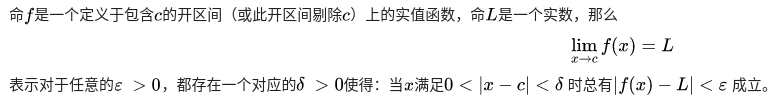
\includegraphics[width=15cm]{pictures_bitmap/wiki_limite.png}
\end{center}
Même pas besoin de connaitre la langue pour comprendre qu'il s'agit bien d'une limite épointée.
 
Contrairement à ce que certains laissent entendre, adopter la limite épointée n'est pas céder à la tradition anlgo-saxonne. C'est juste ce qui se fait partout.

On pourrait penser que ceci n'est pas un élément très lourd au dossier parce qu'il y a moyen d'être très bien tout en étant une spécificité française. C'est le cas par exemple de la notation \( \mathopen] a , b \mathclose[\) pour l'intervalle ouvert.

%///////////////////////////////////////////////////////////////////////////////////////////////////////////////////////////
\subsubsection{La limite épointée est plus riche}
%///////////////////////////////////////////////////////////////////////////////////////////////////////////////////////////

La classe des fonction admettant une limite pointée est plus grande que celle admettant une limite épointée (lemme \ref{LEMooWAZLooDPvemu}). L'utilisation de la limite épointée permet de décrire quelque cas supplémentaires par rapport à ce que l'on peut faire seulement avec la limite pointée.

Pour être plus précis, comme je le disait précédemment, en \ref{NORMooSLAJooLfDreV}, aucune des deux notions n'est satisfaisante seule :
\begin{itemize}
    \item mettez de la limite pointée dans les hypothèses, vous aurez un théorème moins général;
    \item mettez de la limite pointée dans la thèse, vous aurez un résultat plus fort.
\end{itemize}

Le vrai intérêt de la limite épointée est que \emph{en combinaison avec la notion de continuité} permet d'être plus général et plus précis que ce qu'on peut obtenir avec la limite pointée. Dit autrement, le couple (limite épointée, continuité) est plus fort que le couple (limite pointée, continuité).

D'un certain point de vue, oui, la limite pointée est plus simple, mais elle est plus simple parce qu'elle donne moins d'informations.

%///////////////////////////////////////////////////////////////////////////////////////////////////////////////////////////
\subsubsection{Retour sur le théorème de composition}
%///////////////////////////////////////////////////////////////////////////////////////////////////////////////////////////

Le \emph{vrai} théorème de composition est le théorème \ref{THOooHXGIooBclAHA}. Lui, il passe en revue tous les cas possibles et donne le plus de conclusions possibles dans chaque cas.

Ce théorème s'exprime de façon à peu près convenable à l'aide de limites et de continuité. J'attends de voir le même avec une limite pointée et la continuité.

Je suis très ouvert à la discussion si c'est pour avoir quelque chose de plus simple produisant les mêmes résultats. Je ne suis par contre pas très ouvert pour avoir quelque chose de plus simple, mais donnant moins de résultats. C'est toujours facile d'avoir des résultats plus courts, plus simples et plus intuitifs quand on se contente de moins.

%///////////////////////////////////////////////////////////////////////////////////////////////////////////////////////////
\subsubsection{La question est pédagogique}
%///////////////////////////////////////////////////////////////////////////////////////////////////////////////////////////

Tant qu'on ne m'a pas montré comment on exprime le théorème de composition \ref{THOooHXGIooBclAHA} avec des limites pointées, je resterai sur cette idée : la limite pointée est plus simple, mais elle dit moins.

Cela n'est cependant pas spécialement bloquant. Après tout, ça dépend de ce qu'on veut. D'un point de vue pédagogique, la limite pointée introduit autant de \( \epsilon\) et de \( \delta\) qu'on le veut, et permet d'introduire tous les concepts utiles en analyse.

La question est de savoir à quel point on est prêt à se compliquer la vie pour avoir des théorèmes un micro-cheveu plus complets. Le choix du Frido est de recevoir la difficulté avec résignation et de l'endurer avec courage, pour le plaisir d'avoir des théorèmes qui donnent un peu plus d'information\footnote{C'est une de mes citation préférées. Vu que nous sommes entre adultes je vous donne la référence : \cite{BIBooTOVWooSDsNrc}. Si vous n'avez pas 18 ans, on peut vraiment se demander si le Frido sont vraiment des lectures de votre âge.}.


%///////////////////////////////////////////////////////////////////////////////////////////////////////////////////////////
\subsubsection{En fait ça ne change presque rien}
%///////////////////////////////////////////////////////////////////////////////////////////////////////////////////////////

Certains s'imaginent qu'utiliser la limite pointée demande d'ajuster beaucoup de résultats un peu partout\cite{BIBooTOVWooSDsNrc}. Le Frido contient à ma connaissance seulement deux théorèmes dont l'énoncé contient une subtilité due au choix épointé. Le fameux théorème de composition \ref{THOooNPBQooEMOYpd}, et le lemme \ref{LEMooYLIHooFBQyzC}.

Le fait est que l'on ne calcule presque jamais de limites en une valeur où la fonction existe. Si on calcule une limite, c'est précisément parce qu'on regarde un point où la fonction n'existe pas.

Exemples:
\begin{itemize}
    \item Quand on calcule une dérivée, on calcule
        \begin{equation}
            \lim_{\epsilon\to 0}\frac{ f(a+\epsilon)-f(a) }{ \epsilon }.
        \end{equation}
        Cette fonction de \( \epsilon\) n'existe pas lorsque \( \epsilon=0\). Donc les limites pointées et épointées sont identiques.
    \item
        De même, l'étude du sinus cardinal \( f(x)=\sin(x)/x\) (lemme \ref{LEMooMJFBooAjtNjV}) est une fonction dont ça ne viendrait à l'idée de personne de calculer la limite pour \( x\to 4\). Et ça tombe bien : la seule limite que ça donne envie de calculer est
        \begin{equation}
            \lim_{x\to 0} \frac{ \sin(x) }{ x }.
        \end{equation}
        Et encore une fois, la fonction dans le limite n'existe pas au point limite.
    \item
        Toutes les conditions d'intégrabilité demandent des limites à l'infini. Là encore, ce sont des limites vers des points où la fonction n'existe pas. Franchement, qui va vouloir définir
        \begin{equation}
            \begin{aligned}
                f\colon \mathopen[ 0 , \infty \mathclose]&\to \eR \\
                x&\mapsto \begin{cases}
                    x^2    &   \text{si } x\neq \infty\\
                    0    &    \text{si } x=\infty
                \end{cases}
            \end{aligned}
        \end{equation}
        sans rigoler ?  Ok. Pour cette fonction, il y a une différence entre la limite pointée et épointée. Mais franchement, c'est bien la limite épointée qui donne le résultat «intuitif».
\end{itemize}


%///////////////////////////////////////////////////////////////////////////////////////////////////////////////////////////
\subsubsection{Et les filtres ?}
%///////////////////////////////////////////////////////////////////////////////////////////////////////////////////////////

Si vous ne savez pas ce qu'est un filtre, vous pouvez sauter ces paragraphes. Sinon, vous pouvez vous dire que le débat «limite pointée» contre «limite épointée» n'a aucun sens parce que de toutes façons, la bonne façon de définir une limite passe par des filtres.

Alors le mieux est de se demander comment on construit, à partir de la notion de filtre, le nombre \( \lim_{x\to a} f(a)\) ?

Pas de bol, ça dépend du filtre choisi. Le premier filtre auquel on pense pour trouver une définition raisonnable de la limite de \( f(x)\) quand \( x\to a\) est le filtre des voisinages de \( a\). La notion de limite associée est la limite pointée. En ce sens la limite pointée est plus naturelle\cite{BIBooWYHRooVGYMKV,BIBooHHPXooWbCAXQ} que la limite épointée. Cependant «naturel» signifie souvent «le premier qui nous tombe sous la main», ce qui ne signifie pas spécialement «le plus intéressant à utiliser».

La notion de limite épointée est la limite associée au filtre des voisinages épointés. Ce n'est, certes, pas le premier filtre qui nous tombe sous la main, mais il est, au moins dans le cadre de l'étude des fonctions sur \( \eR^n\), le plus efficace; celui qui donne le plus de nouvelles informations par rapport à la continuité.


%///////////////////////////////////////////////////////////////////////////////////////////////////////////////////////////
\subsubsection{En très résumé}
%///////////////////////////////////////////////////////////////////////////////////////////////////////////////////////////

Si vous ne voulez pas lire toute ma prose, voici mes arguments en très court.
\begin{enumerate}
    \item
        La limite épointée est celle utilisée partout sauf en France.
    \item
        La limite épointée est un peu plus compliquée que la limite pointée, mais elle permet de prouver plus de choses. En témoigne le théorème «complèt» de composition \ref{THOooHXGIooBclAHA} que je doute être facile à exprimer à l'aide des limites pointées et de la continuité\footnote{Il y a bien entendu moyen. Voir par exemple \cite{BIBooDAGXooRltbgK}. Sans ironie, je trouve ce théorème fascinant.}.
\end{enumerate}


%///////////////////////////////////////////////////////////////////////////////////////////////////////////////////////////
\subsubsection{Que devez-vous faire ?}
%///////////////////////////////////////////////////////////////////////////////////////////////////////////////////////////

\begin{description}
    \item[Enseignement en France] La notion de limite pointée est celle nommée «limite» dans les programmes, et ce que nous nommons ici «limite» est nommé «limite épointée». Peut-être pour induire en erreur tout le reste de la planète ?
    \item[Recherche] Si vous faites de la recherche où que ce soit y compris en France, la seule définition de limite est la limite dite «épointée», celle qui sera toujours utilisée dans le Frido.
    \item[Doctorat] Vous commencez un doctorat en math, et vous avez vu la limite pointée comme seule définition de limite durant vos études ? Oubliez-la. Ou alors attendez-vous à vous à de sérieux quiproquos lorsque vous discuterez de mathématique avec des étrangers. 

        Disons clairement que si vous utilisez la limite pointée devant des non Français, ils se diront juste que vous devriez relire vos cours de base. Et si vous leur expliquez, il y a de bonnes chance qu'ils ne vous croient pas.
\end{description}



%+++++++++++++++++++++++++++++++++++++++++++++++++++++++++++++++++++++++++++++++++++++++++++++++++++++++++++++++++++++++++++ 
\section{Limites en l'infini}
%+++++++++++++++++++++++++++++++++++++++++++++++++++++++++++++++++++++++++++++++++++++++++++++++++++++++++++++++++++++++++++

Non, sur \( \eR\) nous n'allons pas ajouter \( \infty\) avec la topologie d'Alexandrov de la définition \ref{PROPooHNOZooPSzKIN}. Nous n'allons pas considérer \( \hat \eR=\eR\cup\{ \infty \}\).

\begin{definition}[Droite réelle achevée\cite{ooDZRQooPpOXhY}]       \label{DEFooRUyiBSUooALDDOa}
    Nous considérons l'ensemble
    \begin{equation}
        \bar \eR=\eR\cup\{ +\infty,-\infty \}
    \end{equation}
    où \( +\infty\) et \( -\infty\) ne sont pas des éléments de \( \eR\).

    Nous mettons sur \( \bar\eR\) la relation d'ordre en prenant celle de \( \eR\) à laquelle nous ajoutons les règles
    \begin{enumerate}
        \item
            \( -\infty<x\) pour tout \( x\in\eR\cup\{ +\infty \}\)
        \item
            \( +\infty>x\) pour tout \( x\in \eR\cup\{-\infty  \}\).
    \end{enumerate}

    Nous mettons une topologie sur \( \bar\eR\) en donnant la base\footnote{Base de topologie, définition \ref{DEFooLEHPooIlNmpi}.} suivante :
    \begin{itemize}
        \item \( \mathopen] a , b \mathclose[\),
        \item \( \mathopen] a , +\infty \mathclose]\),
        \item \( \mathopen[ -\infty , b \mathclose[\)
    \end{itemize}
    pour tout réels \( a\) et \( b\).
\end{definition}

\begin{normaltext}
    En principe, la notation «\( \infty\)» est réservée à l'infini du compactifié d'Alexandrov\footnote{Le compactifié d'Alexandrov \( \hat \eR\), définition \ref{PROPooHNOZooPSzKIN}.}, et pour les infinis de la droite réelle achevée, il faudrait bien écrire «\( +\infty\)» et «\( -\infty\)». Cependant, nous allons souvent écrire \( \lim_{x\to \infty} \) au lieu de \( \lim_{x\to +\infty} \).
\end{normaltext}

\begin{lemma}[\cite{MonCerveau}]
    La topologie sur \( \eR\) induite de celle sur \( \bar \eR\) est la topologie usuelle.
\end{lemma}

\begin{proof}
    Nous notons \( \tau_{\eR}\) la topologie de \( \eR\), \( \tau_{\bar \eR}\) celle de \( \bar \eR\) et \( \tau_i\) celle induite de \( \bar \eR\) sur \( \eR\). Nous devons prouver que \( \tau_i=\tau_{\eR}\).
    
    \begin{subproof}
        \item[\( \tau_i\subset\tau_{\eR}\)]
            Un élément de \( \tau_i\) est de la forme \( \mO=\eR\cap A\) où \( A\) est un élément de \( \tau_{\bar \eR}\). Vu que \( A\) est un ouvert de \( \bar \eR\), il est une réunion d'éléments de la base de topologie\footnote{C'est la proposition \ref{DEFooLEHPooIlNmpi} qui dit ça.}; donc \( A=\bigcup_{i\in I}A_i\) où les \( A_i\) sont des trois types listés dans la définition \ref{DEFooRUyiBSUooALDDOa}.
            \begin{enumerate}
                \item
                Si \( A_i=\mathopen] a , b \mathclose[\) alors \( \eR\cap A=\mathopen] a , b \mathclose[\) est un ouvert de \( \eR\).
            \item Si \( A_i=\mathopen] a , +\infty \mathclose]\), alors \( \eR\cap A_i=\mathopen] a , +\infty \mathclose[\) est un ouvert de \( \eR\).
                \item Si \( A_i=\mathopen[ -\infty , b \mathclose[\), même chose.
            \end{enumerate}
            Donc \( \eR\cap A=\bigcup_{i\in I}(\eR\cap A_i)\) est une union d'ouverts de \( \eR\).
        \item[\( \tau_{\eR}\subset\tau_i\)]
        Vu que les \( \mathopen] a , b \mathclose[\) est une base de topologie de \( \eR\), l'ensemble \( \tau_i\) contient une base de topologie de \( \eR\) et donc contient tout \( \tau_{\eR}\).
    \end{subproof}
\end{proof}

\begin{proposition}[\cite{MonCerveau}]
    Soit une suite \( (x_k)\) dans \( \bar \eR=\eR\cup\{ \pm\infty \}\). Nous avons \( x_k\stackrel{\bar \eR}{\longrightarrow}+\infty\) si et seulement si pour tout \( M>0\) il existe un \( N>0\) tel que \( n\geq N\) implique \( x_n>M\).
\end{proposition}

\begin{proof}
    En deux parties.
    \begin{subproof}
        \item[\( \Rightarrow\)]
            Pour tout voisinage \( A\) de \( +\infty\), il existe un \( N\) tel que \( n\geq N\) implique \( x_n\in A\). Soit donc le voisinage \( \mathopen] M , +\infty \mathclose]\), et le \( N\) correspondant. Nous avons alors, pour tout \( n\geq N\), \( x_n\in \mathopen] M , +\infty \mathclose]\) et donc \( x_n\geq M\).
        \item[\( \Leftarrow\)]
        Soit un ouvert \( A\) contenant \( +\infty\). Nous avons \( A=\bigcup_{i\in I} A_i\) où les \( A_i\) sont des trois types listés dans la définition \ref{DEFooRUyiBSUooALDDOa}. Vu que \( +\infty\in A\), pour au moins un des \( i\) nous avons \( A_i=\mathopen] a , +\infty \mathclose[\).

            Prenons \( N\) tel que \( n\geq N\) implique \( x_n>a\). Alors pour \( n\geq N\) nous avons \( x_n\in A\).
    \end{subproof}
\end{proof}

\begin{lemma}       \label{LEMooFCIXooJuHFqk}
    Nous considérons l'espace topologique de la droite réelle achevée\footnote{Définition \ref{DEFooRUyiBSUooALDDOa}.} \( \bar \eR\). Si \( n\geq 1\) nous avons 
    \begin{equation}        \label{EQooRRFEooLYcuRP}
        \lim_{x\to +\infty} x^n = +\infty
    \end{equation}
    et
    \begin{equation}
        \lim_{x\to +\infty} \frac{1}{ x^n }=0.
    \end{equation}
\end{lemma}

\begin{proof}
    Si \( V\) est un voisinage de \( +\infty\), alors nous devons montrer qu'il existe un voisinage \( W\) de \( +\infty\) tel que \( x^n\in V\) pour tout \( x\in W\).   

    Un ouvert est une union d'éléments de la base de topologie\footnote{C'est la définition \ref{DEFooLEHPooIlNmpi}.}. Nous voyons que \( V\) contient au moins une partie de la forme \( \mathopen] R , +\infty \mathclose]\). Nous supposons que \( R>1\).

    Si \( x>R>1\), alors nous avons \( x^n>x\) et donc
    \begin{equation}
        x^n> x>R,
    \end{equation}
    ce qui signifie \( x\in V\).

    En prenant \( W=\mathopen] R , +\infty \mathclose]\), nous avons bien \( W^n\subset V\). Cela prouve \eqref{EQooRRFEooLYcuRP}.

    En ce qui concerne la seconde limite, la démonstration est du même type. Remarquez seulement que vous n'avez pas formellement le droit d'utiliser la proposition \ref{PROPooOUPNooTrClHw} en invoquant \( \frac{1}{ +\infty }=0\).
\end{proof}

%---------------------------------------------------------------------------------------------------------------------------
\subsection{Limite en des nombres}
%---------------------------------------------------------------------------------------------------------------------------

Nous posons la définition suivante.
\begin{definition}      \label{DefInfNombre}
Lorsque $a\in\eR$, on dit que la fonction $f$ \defe{tend vers l'infini quand $x$ tend vers $a$}{} si
\[
  \forall M\in\eR,\exists \delta\tq (| x-a |\leq \delta )\Rightarrow f(x)\geq M\text{ quand }x\in\dom f.
\]
\end{definition}
Cela signifie que l'on demande que dès que $x$ est assez proche de $a$ (c'est-à-dire dès que $| x-a |\leq\delta$), alors $f(x)$ est plus grand que $M$, et que l'on peut trouver un $\delta$ qui fait ça pour n'importe quel $M$. Une autre façon de le dire est que pour toute hauteur $M$, on peut trouver un intervalle de largeur $\delta$ autour de $a$\footnote{C'est-à-dire un intervalle de la forme $[a-\delta,a+\delta]$.} tel que sur cet intervalle, la fonction $f$ est toujours plus grande que $M$.

Montrons sur un dessin pourquoi je disais que la fonction $x\to 1/x$ n'est pas de ce type.


Le problème est qu'il n'existe par exemple aucun intervalle autour de $0$ sur lequel $f$ serait toujours plus grande que $10$. En effet n'importe quel intervalle autour de $0$ contient au moins un nombre négatif. Or quand $x$ est négatif, $f$ n'est certainement pas plus grande que $10$. Nous y reviendrons.

Pour l'instant, montrons que la fonction $f(x)=1/x^2$ est une fonction qui vérifie la définition~\ref{DefInfNombre}.  Avant de prendre n'importe quel $M$, prenons par exemple $100$. Nous avons besoin d'un intervalle autour de zéro sur lequel $f$ est toujours plus grande que $100$. C'est vite vu que $f(0.1)=f(-0.1)=100$, donc l'intervalle $[-\frac{ 1 }{ 10 },\frac{1}{ 10 }]$ est le bon. Partout dans cet intervalle, $f$ est plus grande que $100$. Partout ? Ben non : en $x=0$, la fonction n'est même pas définie, donc c'est un peu dur de dire qu'elle est plus grande que $100$. C'est pour cela que nous avons ajouté la condition « quand $x\in\dom f$ » dans la définition de la limite.

Prenons maintenant un $M\in\eR$ arbitraire, et trouvons un intervalle autour de $0$ sur lequel $f$ est toujours plus grande que $M$. La réponse est évidemment l'intervalle de largeur $1/\sqrt{M}$, c'est-à-dire
\[
  \left[ -\frac{ 1 }{ \sqrt{M} },\frac{ 1 }{ \sqrt{M} } \right].
\]

\subsection{Limites quand tout va bien}
%--------------------------------------

D'abord définissons ce qu'on entend par la limite d'une fonction en un point quand il n'y a aucun infini en jeu.
\begin{definition}      \label{DefLimPointSansInfini}
 On dit que la fonction $f$ \defe{tend vers $b$ quand $x$ tend vers $a$}{} si
\[
  \forall \epsilon>0,\exists\delta\tq (| x-a |\leq\delta)\Rightarrow | f(x)-b |\leq \epsilon\text{ quand }x\in\dom f.
\]
Dans ce cas, nous notons
\begin{equation}
\lim_{x\to a}f(x)=b.
\end{equation}
\end{definition}

Commençons par un exemple très simple : prouvons que $\lim_{x\to 0}x=0$. C'est donc $a=b=0$ dans la définition. Prenons $\epsilon>0$, et trouvons un intervalle autour de zéro tel que partout dans l'intervalle, $x\leq \epsilon$. Bon ben c'est clair que $\delta=\epsilon$ fonctionne.

Plus compliqué maintenant, mais toujours sans surprises.

\begin{proposition}
\[
  \lim_{x\to 0}x^2=0.
\]

\end{proposition}

\begin{proof}
Soit $\epsilon>0$. On veut un intervalle de largeur $\delta$ autour de zéro tel que $x^2$ soit plus petit que $\epsilon$ sur cet intervalle. Cette fois-ci, le $\delta$ qui fonctionne est $\delta=\sqrt{\epsilon}$. En effet un élément de l'intervalle $[-\delta,\delta]$ est un $r$ de valeur absolue plus petite ou égale à $\delta$ :
\[
| r |\leq\delta=\sqrt{\epsilon}.
\]
En prenant le carré de cette inégalité on a :
\[
  r^2\leq\epsilon,
\]
ce qu'il fallait prouver.
\end{proof}

Calculer et prouver des valeurs de limites, mêmes très simples, devient vite de l'arrachage de cheveux à essayer de trouver le bon $\delta$ en fonction de $\epsilon$ si on n'a pas quelques théorèmes généraux. Heureusement nous en avons déjà quelques uns : \ref{PROPooVLBWooVttvFK}, \ref{PROPooDQFIooMMwxxJ}, \ref{ThoLimLinMul}, \ref{ThoLimLin}, \ref{PROPooOUPNooTrClHw}.

\begin{proposition}[\cite{MonCerveau}]      \label{PROPooWXBAooAEweSF}
    Soit \( f\colon \eR^2\to \eR\) une application continue dont la variable \( y\) varie dans un compact \( I\) de \( \eR\). Alors la fonction
    \begin{equation}
        \begin{aligned}
            d\colon \eR&\to \eR \\
            x&\mapsto \sup_{y\in I} f(x,y)
        \end{aligned}
    \end{equation}
    est continue.
\end{proposition}

\begin{proof}
    Soit \( x_0\) fixé. Prouvons que \( d\) est continue en \( x_0\). Nous notons \( y_0\) la valeur de \( y\) qui réalise le maximum (par le théorème~\ref{ThoMKKooAbHaro} et le fait que les fonctions projection soient continues, lemme~\ref{LEMooHAODooYSPmvH}). Soit aussi \( \epsilon>0\) tellement fixé que même avec un tourne vis hydraulique, il ne bougerait pas. Nous considérons \( \delta\) tel que si \( \| (x,y)-(x_0,y_0) \|\leq \delta\) alors \( \| f(x,y)-f(x_0,y_0) \|<\epsilon\).

    Si \( | x-x_0 |<\delta\) alors pour \( y\) assez proche de \( y_0\) nous avons \( \| (x,y)-(x_0,y_0) \|\leq \delta\), et donc \( \| f(x,y)-f(x_0,y_0) \|\leq \epsilon \). Cela montre qu'il existe \( \delta\) tel que \( | x-x_0 |\leq \delta\) implique \( d(x)\geq d(x_0)-\epsilon\).

    Nous devons encore trouver un \( \delta\) tel que si \( | x-x_0 |\leq \delta\) alors \( d(x)\leq d(x_0)+\epsilon\). Supposons que non. Alors pour tout \( \delta\) il existe un \( x\) tel que \( | x-x_0 |\leq \delta\) et \( d(x)> d(x_0)+\epsilon\). Cela nous donne une suite \( x_i\to x_0\).

    Pour chaque \( x_i\) nous notons \( y_i\) la valeur de \( y\) qui réalise le supremum correspondant. La suite \( (y_i)\) étant contenue dans un compact nous supposons prendre une sous-suite de \( (x_i)\) telle que la suite \( (y_i)\) converge. Nous nommons \( a\) la limite (et non \( y_0\) parce que nous ne savons pas si \( y_i\to y_0\)). Pour chaque \( i\) nous avons
    \begin{equation}
        f(x_i,y_i)>\sup_{y\in I}f(x_0,y)+\epsilon.
    \end{equation}
    En prenant la limite et en utilisant la continuité de \( f\),
    \begin{equation}
        f(x_0,a)>\sup_{y\in I} f(x_0,y)+\epsilon,
    \end{equation}
    ce qui est impossible.
\end{proof}

%---------------------------------------------------------------------------------------------------------------------------
\subsection{Limites de fonctions}
%---------------------------------------------------------------------------------------------------------------------------

Tentons de comprendre ce que signifie qu'un nombre $\ell$ \emph{ne soit pas} la limite de $f$ lorsque $x\to a$. Il s'agit d'inverser la condition de la proposition \ref{PropHOCWooSzrMjl}\ref{ITEMooSHKNooStKGKH}. Le nombre $\ell$ n'est pas une limite de $f$ pour $x\to a$ lorsque
\begin{equation}		\label{EqCaractNonLim}
	\exists\varepsilon>0\tq\,\forall\delta>0,\,\exists x\tq 0<\| x-a \|<\delta\text{ et }\| f(x)-\ell \|>\varepsilon,
\end{equation}
c'est-à-dire qu'il existe un certain seuil $\varepsilon$ tel qu'on a beau s'approcher aussi proche qu'on veut de $a$ (distance $\delta$), on trouvera toujours un $x$ tel que $f(x)$ n'est pas $\varepsilon$-proche de $\ell$.

\begin{lemma}[Unicité de la limite]
	Si $\ell$ et $\ell'$ sont deux limites de $f(x)$ lorsque $x$ tend vers $a$, alors $\ell=\ell'$.
\end{lemma}

\begin{proof}
	Soit $\varepsilon>0$. Nous considérons $\delta$ tel que $\| f(x)-\ell \|<\varepsilon$ pour tout $x$ tel que $\| x-a \|<\delta$. De la même manière, nous prenons $\delta'$ tel que $\| x-a \|<\delta'$ implique $\| f(x)-\ell' \|<\varepsilon$. Pour les $x$ tels que $\| x-a \|$ est plus petit que $\delta$ et $\delta'$ en même temps, nous avons
	\begin{equation}
		\| \ell-\ell' \|=\| \ell-f(x)+f(x)-\ell' \|\leq\| \ell-f(x) \|+\| f(x)-\ell' \|<2\varepsilon,
	\end{equation}
	et donc $\| \ell-\ell' \|=0$ parce que c'est plus petit que $2\varepsilon$ pour tout $\varepsilon$.
\end{proof}

\begin{proposition}[\cite{MonCerveau}]  \label{PROPooKPOXooEHIXJs}
    Soient un espace vectoriel normé \( (V,\| . \|)\) et \( a\in V\). Soient encore un voisinage \( A\) de \( a\) et deux fonctions \( f,g\colon A\setminus \{ a \}\to \eR\) qui admettent une limite en \( a\). 

    Si \( f(x)\leq g(x)\) pour tout \( x\in A\setminus \{ a \}\) alors 
    \begin{equation}
        \lim_{x\to a} f(x)\leq \lim_{x\to a}f(x).
    \end{equation}
\end{proposition}

%--------------------------------------------------------------------------------------------------------------------------- 
\subsection{Limite à gauche et à droite}
%---------------------------------------------------------------------------------------------------------------------------

Si \( a\) est à l'intérieur du domaine de \( f\), nous savons ce que signifie \( \lim_{x\to a} f(x)\). Nous donnons également une définition des limites à gauche et à droite.

\begin{definition}
    Soient \( D\subset \eR\) et une fonction \( f\colon D\to \eR\). Si \( a\in \Adh(D)\) nous définissons la \defe{limite à droite}{limite à droite} de \( f\) en \( a\) par
    \begin{equation}        \label{EQooQKHLooMoSXVe}
        \lim_{x\to a^+} f(x)=\lim_{x\to a} \tilde f(x)
    \end{equation}
    où \( \tilde f\) est la fonction \( f\) restreinte à \( D\cap\{ x\tq x>a \}\). La limite \eqref{EQooQKHLooMoSXVe} est souvent écrite sous la forme condensée
    \begin{equation}
        \lim_{\substack{x\to a\\x>a}}f(x).
    \end{equation}
    Pour la limite à gauche c'est un peu la même chose :
    \begin{equation}
        \lim_{x\to a^-} f(x)=\lim_{\substack{x\to a\\x<a}}f(x).
    \end{equation}
\end{definition}

\begin{lemma}       \label{LEMooXJMFooCkzoVi}
Soient \( D\subset \eR\) et une fonction \( f\colon D\to \eR\). Si \( a\in \Adh(D)\) nous avons \( \lim_{x\to a^+} f(x)=\ell\) si et seulement si pour tout \( \epsilon>0\), il existe \( \delta>0\) tel que  \( x\in\mathopen] a , a+\delta \mathclose[\cap D\) implique \( f(x)\in B(\ell,\epsilon)\).
\end{lemma}

\begin{proof}
    Nous avons les équivalences entre les faits suivants, en utilisant la définition \ref{DefYNVoWBx} de la limite :
    \begin{enumerate}
        \item
            \( \lim_{x\to a^+} f(x)=\ell\)
        \item
            \( \lim_{x\to a} \tilde f(x)=\ell\)
        \item
            Pour tout \( \epsilon>0\), il existe \( \delta>0\) tel que si \( x\in B(a,\delta)\cap D\cap\{ x>a \}\) alors \( f(x)\in B(\ell,\epsilon)\)
        \item
        Pour tout \( \epsilon>0\), il existe \( \delta>0\) tel que si \( x\in \mathopen] a , a+\delta \mathclose[\cap D\) alors \( f(x)\in B(\ell,\epsilon)\)
    \end{enumerate}
\end{proof}

\begin{proposition}[\cite{ooOMWZooZvUFiG}]      \label{PROPooGDDJooDCmydE}
    Soit une fonction \( f\colon D\to \eR\) où \( D\) est une partie de \( \eR\). Si \( a\in \Adh(D)\) alors la limite \( \lim_{x\to a} f(x)\) existe si et seulement si les limites à gauche et à droite existent et sont égales. Dans ce cas nous avons égalité :
    \begin{equation}
        \lim_{x\to a} f(x)=\lim_{x\to a^+} f(x)=\lim_{x\to a^-} f(x).
    \end{equation}
\end{proposition}

\begin{proof}
    En deux parties.
    \begin{subproof}
        \item[\( \Rightarrow\)]
        Nous disons que \( \lim_{x\to a} f(x)=\ell\). Si \( V\) est un voisinage de \( \ell\), il existe un voisinage \( U\) de \( a\) tel que \( f\big( U\cap D\setminus \{ a \} \big)\subset V\). En particulier il existe un \( \delta>0\) tel que si \( x\in \mathopen] a , a+\delta \mathclose[\cap D\), alors \( | f(x)-\ell |<\epsilon\). Cela est la limite à droite (lemme \ref{LEMooXJMFooCkzoVi}).
        \item[\( \Leftarrow\)]
        Soit \( \epsilon>0\). Par la limite à droite, il existe \( \delta_1>0\) tel que \( f\big( \mathopen] a , a+\delta_1 \mathclose[\cap D \big)\subset B(\ell,\epsilon)\). La la limite à gauche, il existe \( \delta_2\) tel que \( f\big( \mathopen] a-\delta , a \mathclose[\cap D \big)\subset B(\ell,\epsilon)\)

            En prenant \( \delta=\min\{ \delta_1,\delta_2 \}\) nous avons bien \( f\big( B(a,\delta)\cap D\setminus\{ a \} \big)\subset B(\ell,\epsilon)\) comme le demande la définition de la limite.
    \end{subproof}
\end{proof}

\begin{normaltext}
    Quelques remarques à propos de la proposition \ref{PROPooGDDJooDCmydE}.
    \begin{enumerate}
        \item
    Cette proposition ne se généralise pas aux dimensions supérieures. Dans \( \eR^2\) par exemple, il ne faudrait pas croire que si les limites suivant toutes les directions existent alors la limite existe.
\item
    Cette proposition est souvent utilisée pour calculer des limites dans lesquelles arrivent des valeurs absolues. Par exemple durant la démonstration de la proposition \ref{PROPooCNDHooKRwils}.
    \end{enumerate}
\end{normaltext}

%+++++++++++++++++++++++++++++++++++++++++++++++++++++++++++++++++++++++++++++++++++++++++++++++++++++++++++++++++++++++++++ 
\section{Limite en compactifié d'Alexandrov}
%+++++++++++++++++++++++++++++++++++++++++++++++++++++++++++++++++++++++++++++++++++++++++++++++++++++++++++++++++++++++++++

Nous considérons l'espace topologique localement compact \( \eR\), et son compactifié d'Alexandrov défini en \ref{PROPooHNOZooPSzKIN}. Nous avons donc un point supplémentaire noté \( \infty\). Ce point n'est ni du côté des grands nombres positifs, ni du côté des grands nombres négatifs. Il n'est ni \( +\infty\) ni \( -\infty\).

\begin{proposition}
    Dans cet espace topologique \( \hat \eR=\eR\cup\{ \infty \}\),
    \begin{equation}
        \lim_{x\to 0} \frac{1}{ x }=\infty.
    \end{equation}
\end{proposition}

\begin{proof}
    Soit un voisinage \( V\) de \( \infty\) dans \( \hat \eR\). Il s'écrit \( V=K^c\cup\{ \infty \}\) pour un certain compact de \( \eR\). Le théorème \ref{ThoXTEooxFmdI} nous assure que \( K\) est borné. Donc il existe \( R>0\) tel que \( K\subset B(0,R)\). Pour \( x\in B(0,1/R)\) nous avons
    \begin{equation}
        | \frac{1}{ x } |>R,
    \end{equation}
    et donc \( 1/x\in K^c\). Donc aussi \( \frac{1}{ x }\in V\).
\end{proof}

De la même façon, dans \( \eC\cup\{ \infty \}\) nous avons
\begin{equation}
    \lim_{z\to 0} \frac{1}{ z }=\infty.
\end{equation}

\begin{normaltext}
    Je vous laisse deviner la topologie à considérer sur \( \bar \eR=\eR\cup\{ +\infty,-\infty \}\). Dans cet espace topologique la limite \( \lim_{x\to 0} \frac{1}{ x }\) n'existe pas.
\end{normaltext}

%---------------------------------------------------------------------------------------------------------------------------
\subsection{Prolongement par continuité}
%---------------------------------------------------------------------------------------------------------------------------

%///////////////////////////////////////////////////////////////////////////////////////////////////////////////////////////
\subsubsection{Discussion avec mon ordinateur}
%///////////////////////////////////////////////////////////////////////////////////////////////////////////////////////////

Voici un extrait de ce peut donner Sage. Nous lui donnons la fonction
\begin{equation}    \label{EqyEHTBZ}
    f(x)=\frac{ x+4 }{ 3x^2+10x-8 }.
\end{equation}
Cette fonction est faite exprès pour que le dénominateur s'annule en \( -4\). En fait \( 3x^2+10x-8=(x+4)(3x-2)\), et la fraction peut se simplifier en
\begin{equation}
    f(x)=\frac{1}{ 3x-2 }.
\end{equation}
Et avec cela nous écririons \( f(-4)=-\frac{1}{ 14 }\). Voyons comment cela passe dans Sage.

\begin{verbatim}
----------------------------------------------------------------------
| Sage Version 5.2, Release Date: 2012-07-25                         |
| Type "notebook()" for the browser-based notebook interface.        |
| Type "help()" for help.                                            |
----------------------------------------------------------------------
sage: f(x)=(x+4)/(3*x**2+10*x-8)
sage: f(-4)
---------------------------------------------------------------------------
ValueError                                Traceback (most recent call last)
ValueError: power::eval(): division by zero
\end{verbatim}
Il produit donc une erreur de division par zéro. Cela n'est pas étonnant. Pourtant si on lui demande, il est capable de simplifier. En effet :
\begin{verbatim}
sage: f.simplify_full()
x |--> 1/(3*x - 2)
sage: f.simplify_full()(-4)
-1/14
\end{verbatim}

Nous considérons la question suivante : étant donné une fonction \( f\) définie sur \( I\setminus\{ x_0 \}\), est-il possible de définir \( f\) en \( x_0\) de telles façon à ce qu'elle soit continue ?

\begin{example}
    La fonction
    \begin{equation}
        \begin{aligned}
            f\colon \eR\setminus\{ 0 \}&\to \eR \\
            x&\mapsto \frac{1}{ x }
        \end{aligned}
    \end{equation}
    n'est pas définie pour \( x=0\) et il n'y a pas moyen de définir \( f(0)\) de telle sorte que \( f\) soit continue parce que \( \lim_{x\to 0} \frac{1}{ x }\) n'existe pas.
\end{example}

%///////////////////////////////////////////////////////////////////////////////////////////////////////////////////////////
\subsubsection{Limite et prolongement}
%///////////////////////////////////////////////////////////////////////////////////////////////////////////////////////////

Reprenons l'exemple de la fonction \eqref{EqyEHTBZ} que mon ordinateur refusait de calculer en zéro :
\begin{equation}
f(x)=\frac{ x+4 }{ 3x^2+10x-8 }=\frac{ x+4 }{ (x+4)\left( x-\frac{ 2 }{ 3 } \right) }.
\end{equation}
Cette fonction a une condition d'existence en $x=-4$. Et pourtant, tant que $x\neq 4$, cela a un sens de simplifier les $(x+4)$ et d'écrire
\[
  f(x)=\frac{ 1 }{ x-\frac{ 2 }{ 3 } }=\frac{ 3 }{ 3x-2 }.
\]
Étant donné que pour toute valeur de $x$ différente de $-4$, la fonction $f$ s'exprime de cette façon, nous avons que
\[
  \lim_{x\to -4}f(x)=\lim_{x\to -4}\left(\frac{ 3 }{ 3x-2 }\right).
\]
Oui, mais la fonction\footnote{Cette fonction $g$ n'est pas $f$ parce que $g$ a en plus l'avantage d'être définie en $-4$.} $g(x)=3/(3x-2)$ est continue en $-4$ et donc sa limite vaut sa valeur. Nous en déduisons que
\[
  \lim_{x\to -4}f(x)=-\frac{ 3 }{ 14 }.
\]
Que dire maintenant de la fonction ainsi définie ?
\begin{equation}
\tilde f(x)=
\begin{cases}
f(x)&\text{si }x\neq -4\\
-3/14&\text{si }x=-4.
\end{cases}
\end{equation}
Cette fonction est continue en $-4$ parce qu'elle y est égale à sa limite. Les étapes suivies pour obtenir ce résultat sont :
\begin{itemize}
\item Repérer un point où la fonction n'existe pas,
\item calculer la limite de la fonction en ce point, et en particulier vérifier que cette limite existe, ce qui n'est pas toujours le cas,
\item définir une nouvelle fonction qui vaut partout la même chose que la fonction originale, sauf au point considéré où l'on met la valeur de la limite.
\end{itemize}
C'est ce qu'on appelle \defe{prolonger la fonction par continuité}{prolongement!par continuité} parce que la fonction résultante est continue. La prolongation de $f$ par continuité est donc en général définie par
\begin{equation}
\tilde f(x)=
\begin{cases}
f(x)            &\text{si }f(x)\\
\lim_{y\to x}f(y)   &\text{si }f(x)
\end{cases}
\end{equation}
Dans le cas que nous regardions,
\[
    f(x)=\frac{ x+4 }{ 3x^2+10x-8 },
\]
le prolongement par continuité est donné par
\begin{equation}
\tilde f =\frac{ 3 }{ 3x-2 }.
\end{equation}
Remarquons que cette fonction n'est toujours pas définie en $x=2/3$.

%---------------------------------------------------------------------------------------------------------------------------
\subsection{Prolongement par continuité}
%---------------------------------------------------------------------------------------------------------------------------

\begin{propositionDef}[Prolongement par continuité]
    Soit \( f\colon I\setminus\{ x_0 \}\to \eR\) telle que \( \lim_{x\to x_{0}} f(x)=\ell\in \eR\). La fonction
    \begin{equation}
        \begin{aligned}
            \tilde f\colon I&\to \eR \\
            \tilde f(x)&=\begin{cases}
                f(x)    &   \text{si } x\neq x_0\\
                \ell    &    \text{si } x=x_0
            \end{cases}
        \end{aligned}
    \end{equation}
    est une fonction continue sur \( I\) et est appelée le \defe{prolongement par continuité}{prolongement!par continuité} de \( f\) en \( x_0\).
\end{propositionDef}
Vous noterez que dans cet énoncé nous demandons \( \ell\in \eR\). Les cas \( \ell=\pm\infty\) sont donc exclus.

\begin{normaltext}
    Le lemme~\ref{LEMooUAFBooAwiXxj} donnera un autre gros morceau de prolongement par continuité. Là, ce ne sera pas juste une valeur qui manquera, mais carrément la majorité des valeurs; mais par contre, ce ne sera pas vraiment de la prolongation par continuité, mais de la prolongation par Cauchy-continuité.
\end{normaltext}

\begin{example}
    La fonction
    \begin{equation}
        \begin{aligned}
            f\colon \eR\setminus\{ -3,2 \}&\to \eR \\
            x&\mapsto  \frac{ x^2+2x-3 }{ (x+3)(x-2) }
        \end{aligned}
    \end{equation}
    admet pour limite \( \lim_{x\to -3} f(x)=\frac{ 4 }{ 5 }\). Son prolongement par continuité en \( x=-3\) est donné par
    \begin{equation}
        \tilde f(x)=\frac{ x-1 }{ x-2 }.
    \end{equation}
    Notons que les fonctions \( f\) et \( \tilde f\) ne sont pas identiques : l'une est définie pour \( x=-3\) et l'autre pas. Lorsqu'on fait le calcul
    \begin{equation}
        \frac{ x^2+2x-3 }{ (x+3)(x-2) }=\frac{ (x-1)(x+3) }{ (x+3)(x-2) }=\frac{ x-1 }{ x-2 },
    \end{equation}
    la simplification n'est pas du tout un acte anodin. Le dernier signe «\( =\)» est discutable parce que les deux dernières expressions ne sont pas égales pour tout \( x\); elles ne sont égales «que» pour les \( x\) pour lesquels les deux expressions existent.
\end{example}

Les fonctions trigonométriques donneront quelques exemples intéressants de prolongements par continuité. Voir l'exemple~\ref{ExQWHooGddTLE}. Et une avec la fonction logarithme dans l'exemple~\ref{EXooAGEOooQdQkrS}.

%---------------------------------------------------------------------------------------------------------------------------
\subsection{Théorème de la bijection}
%---------------------------------------------------------------------------------------------------------------------------

\begin{proposition} \label{PropOARooUuCaYT}
    Une fonction monotone et surjective d'un intervalle $I$ sur un autre intervalle $J$ est continue sur $I$.
\end{proposition}

\begin{proposition}
    Soient \( f\colon I\to J\) une bijection et \( f^{-1}\colon J\to I\) sa réciproque. Alors pour tout \( x_0\in I\) nous avons
    \begin{equation}    \label{EqHQRooNmLYbF}
        f^{-1}\big( f(x_0) \big)=x_0
    \end{equation}
    et pour tout \( y_0\in J\) nous avons
    \begin{equation}    \label{EqIYTooQPvZDr}
        f\big( f^{-1}(y_0) \big)=y_0.
    \end{equation}
\end{proposition}

\begin{proof}
    Nous prouvons la relation \eqref{EqHQRooNmLYbF} et nous laissons \eqref{EqIYTooQPvZDr} comme exercice au lecteur.

    Soit \( x_0\in I\). Posons \( y_0=f(x_0)\). La définition de l'application réciproque est que pour \( y\in J\), \( f^{-1}(y)\) est l'unique élément \( x\) de \( I\) tel que \( f(x)=y\). Donc \( f^{-1}(y_0)\) est l'unique élément de \( I\) dont l'image est \( y_0\). C'est donc \( x_0\) et nous avons \( f^{-1}(y_0)=x_0\), c'est-à-dire
    \begin{equation}
        f^{-1}\big( f(x_0) \big)=x_0.
    \end{equation}
\end{proof}

\begin{theorem}[Théorème de la bijection] \label{ThoKBRooQKXThd}
    Soit $I$ un intervalle et $f$ une fonction continue et strictement monotone de $I$ dans \( \eR\). Nous avons alors :
    \begin{enumerate}
        \item
            $f(I)$ est un intervalle de \( \eR\) ;
        \item       \label{ITEMooMAWXooZXmVwA}
            La fonction \( f\colon I\to f(I)\) est bijective
        \item
            La fonction \( f^{-1}\colon f(I)\to I\) est strictement monotone de même sens que $f$ ;
        \item \label{ItemEJZooKuFoeFiv}
            La fonction \( f\colon I\to f(I)\) est un homéomorphisme, c'est-à-dire que \( f^{-1}\colon f(I)\to I\) est continue.
    \end{enumerate}
\end{theorem}

\begin{proof}

    Prouvons les choses point par point.

    \begin{enumerate}
    \item

        Supposons pour fixer les idées que \( f\) est monotone croissante\footnote{Traitez en tant qu'exercice le cas où $ f$ est décroissante.}.

        Soient \( a< b\) dans \( f(I)\). Par définition il existe \( x_1,x_2\in I\) tels que \( a=f(x_1)\) et \( b=f(x_2)\). La fonction \( f\) est continue sur l'intervalle \( \mathopen[ x_1 , x_2 \mathclose]\) et vérifie \( f(x_1)<f(x_2)\). Donc le théorème des valeurs intermédiaires~\ref{ThoValInter} nous dit que pour tout \( t\) dans \( \mathopen[ f(x_2) , f(x_2) \mathclose]\), il existe un \( x_0\in\mathopen[ x_1 , x_2 \mathclose]\) tel que \( f(x_0)=t\). Cela montre que toutes les valeurs intermédiaires entre \( a\) et \( b\) sont atteintes par \( f\) et donc que \( f(I)\) est un intervalle.

    \item

    Nous prouvons maintenant que \( f\) est bijective en prouvant séparément qu'elle est surjective et injective.

    \begin{subproof}

        \item[\( f\) est surjective]

            Une fonction est toujours surjective depuis un intervalle \( I\) vers l'ensemble \(\Im f \).

        \item[\( f\) est injective]

            Soit \( x\neq y\) dans \( I\); pour fixer les idées nous supposons que \( x<y\). La stricte monotonie de \( f\) implique que \( f(x)<f(y)\) ou que \( f(x)>f(y)\). Dans tous les cas \( f(x)\neq f(y)\).

    \end{subproof}

    La fonction \( f\) est donc bijective.

\item

    Comme d'accoutumée nous supposons que \( f\) est croissante. Soient \( y_1<y_2\) dans \( f(I)\); nous devons prouver que \( f^{-1}(y_1)\leq f^{-1}(y_2)\). Pour cela nous considérons les nombres \( x_1,x_2\in I\) tels que \( f(x_1)=y_1\) et \( f(x_2)=y_2\). Nous allons en prouver la contraposée en supposant que \( f^{-1}(y_1)>f^{-1}(y_2)\). En appliquant \( f\) (qui est croissante) à cette dernière inégalité il vient
    \begin{equation}
        f\big( f^{-1}(y_1) \big)\geq f\big( f^{-1}(y_2) \big),
    \end{equation}
    ce qui signifie
    \begin{equation}
        y_1\geq y_2
    \end{equation}
    par l'équation \eqref{EqIYTooQPvZDr}.

\item

    La fonction \( f^{-1}\colon f(I)\to I\) est une fonction monotone et surjective, donc continue par la proposition~\ref{PropOARooUuCaYT}.

    \end{enumerate}
\end{proof}

\begin{example}
    La fonction
    \begin{equation}
        \begin{aligned}
            f\colon \mathopen[ 2 , 3 \mathclose]&\to \mathopen[ 4 , 9 \mathclose] \\
            x&\mapsto x^2
        \end{aligned}
    \end{equation}
    est une bijection. Sa réciproque est la fonction
    \begin{equation}
        \begin{aligned}
            f^{-1}\colon \mathopen[ 4 , 9 \mathclose]&\to \mathopen[ 2 , 3 \mathclose] \\
            x&\mapsto \sqrt{x}.
        \end{aligned}
    \end{equation}
\end{example}

%+++++++++++++++++++++++++++++++++++++++++++++++++++++++++++++++++++++++++++++++++++++++++++++++++++++++++++++++++++++++++++
\section{Limite et continuité}
%+++++++++++++++++++++++++++++++++++++++++++++++++++++++++++++++++++++++++++++++++++++++++++++++++++++++++++++++++++++++++++
\label{SecLimiteFontion}

Voir les remarques dans l'index thématique~\ref{THEMEooGVCCooHBrNNd} pour comprendre la place et la portée de ce qui va venir à propos de limite et de continuité.

\begin{theorem}[Limite et continuité]           \label{ThoLimCont}
La fonction $f$ est continue au point $a$ si et seulement si $\lim_{x\to a}f(x)=f(a)$.
\end{theorem}

\begin{proof}
    Nous commençons par supposer que $f$ est continue en $a$, et nous prouvons que $\lim_{x\to a}f(x)=a$. Soit $\epsilon>0$; ce qu'il nous faut c'est un $\delta$ tel que $| x-a |\leq\delta$ implique $| f(x)-f(a) |\leq\epsilon$. La caractérisation \ref{PROPooVNGEooPwbxXP} de la continuité donne l'existence d'un $\delta$ comme il nous faut.

    Dans l'autre sens, c'est-à-dire prouver que $f$ est continue au point $a$ sous l'hypothèse que $\lim_{x\to a}f(x)=f(a)$, la preuve se fait de la même façon.
\end{proof}

Nous en déduisons que si nous voulons gagner quelque chose à parler de limites, il faut prendre des fonctions non continues. En effet, si une fonction est continue en un point, la limite ne donne aucune nouvelle information que la valeur de la fonction elle-même en ce point.

Prenons une fonction qui fait un saut. Pour se fixer les idées, prenons celle-ci :
\begin{equation}    \label{EqnCtOEL}
f(x)=
\begin{cases}
2x&\text{si }x\in]\infty,2[\\
x/2&\text{si }x\in[2,\infty[
\end{cases}
\end{equation}
Essayons de trouver la limite de cette fonction lorsque $x$ tend vers $2$. Étant donné que $f$ n'est pas continue en $2$, nous savons déjà que $\lim_{x\to 2}f(x)\neq f(2)$. Donc ce n'est pas $1$. Cette limite ne peut pas valoir $4$ non plus parce que si je prends n'importe quel $\epsilon$, la valeur de $f(2+\epsilon)$ est très proche de $2$, et donc ne peut pas s'approcher de $4$. En fait, tu peux facilement vérifier que \emph{aucun nombre ne vérifie la condition de limite pour $f$ en $2$}. Nous disons que la limite n'existe pas.

Il ne faudrait pas en déduire trop vite que si une fonction n'est pas continue en \( a\), alors la limite \( x\to a\) n'existe pas. Ce que dit le théorème~\ref{ThoLimCont} est que si une fonction n'est pas continue en \( a\), alors sa limite (si elle existe) ne vaut pas \( f(a)\).

\begin{example}[Un exemple de continuité Thème~\ref{THEMEooGVCCooHBrNNd}]     \label{EXooKREUooLeuIlv}
    Soit la fonction
    \begin{equation}        \label{EQooSYSWooSGsUfR}
        f(x)=\begin{cases}
            x    &   \text{si } x\neq 0\\
            4    &    \text{si } x=0.
        \end{cases}
    \end{equation}
    Cette fonction n'est pas continue en \( x=0\), et pourtant la limite existe : \( \lim_{x\to 0} f(x)=0\). Faisons cela en détail pour nous assurer de ce qu'il se passe.

    Considérons l'ouvert \( \mathopen] 3 , 5 \mathclose[\). L'image réciproque de cet ouvert par \( f\) est la partie \( \mathopen] 3 , 5 \mathclose[\cup\{ 0 \}\) qui n'est pas ouvert. Donc la fonction \( f\) n'est pas continue comme fonction \( \eR\to \eR\).

    Considérons pour comprendre la restriction \( f\colon \mathopen[ -1 , 1 \mathclose]\to \eR\). L'image inverse de \( \mathopen] 3 , 5 \mathclose[\) par cette fonction est \( \{ 0 \}\) qui n'est pas un ouvert.

    Plus généralement tant qu'on considère des restrictions de \( f\) sur des parties contenant un voisinage de \( 0\), la fonction ne peut pas être continue\footnote{Les plus acharnés se demanderont ce qu'il se passe pour la restriction de \( f\) à la partie \( \{ 0 \}\) munie de la topologie induite de $\eR$.}.

    Voyons ce qui en est de la continuité ponctuelle de \( f\) en \( x=0\). La définition~\ref{DefOLNtrxB} est celle de la continuité en un point; elle dit que \( f\) sera continue en \( 0\) si \( f(0)=4\) est une limite de \( f\). Nous voila parti vers la définition~\ref{DefYNVoWBx}.

Soit le voisinage \( V=\mathopen] 3 , 5 \mathclose[\) de \( f(0)\). Quel que soit le voisinage \( W\) de \( 0\) dans \( \eR\), il existe un \( \epsilon>0\) tel que \( W\subset B(0,\epsilon)\). Nous avons alors
    \begin{equation}
        f\big( W\setminus \{ a \} \big)\subset f\big( B(0,\epsilon)\setminus\{ 0 \} \big).
    \end{equation}
    Mais le nombre \( \epsilon/2\) fait partie de \( f\big( B(0,\epsilon)\setminus\{ 0 \} \big)\) et n'est pas dans \( V\). Donc \( f(0)\) n'est pas une limite de \( f\) en zéro. Cette fonction n'est donc pas continue en zéro.
\end{example}

\begin{example}[Même exemple, limite]
    Nous avons vu que, pour la fonction \eqref{EQooSYSWooSGsUfR}, le nombre \( 4\) n'est pas une limite de \( f\) en zéro. Nous montrons à présent que \( 0\) est une limite (et même la seule par la proposition~\ref{PropFObayrf} que nous ne rappellerons plus à chaque fois) de \( f\).

    Montrons que \( 0\) est une limite de \( f\) en zéro, c'est-à-dire que \( \lim_{x\to 0} f(x)=0\).

    Nous suivant la définition~\ref{DefYNVoWBx}. Soit un voisinage \( V\) de \( 0\) dans \( \eR\). Il existe \( \delta\) tel que \( B(0,\delta)\subset V\). En posant \( \epsilon=\delta\) et en définissant \( W=B(0,\epsilon)\) nous avons
    \begin{equation}
        f\big( B(0,\epsilon)\setminus\{ 0 \} \big)=B(0,\epsilon)\setminus\{ 0 \}\subset  B(0,\delta)\subset V.
    \end{equation}
    Donc \( 0\) est une limite de \( f\) en zéro.
\end{example}

Nous avons déjà vu par le corolaire~\ref{CorFHbMqGGyi} qu'une suite croissante et bornée était convergente. Il en va de même pour les fonctions.
\begin{proposition}[\cite{MonCerveau}] \label{PropMTmBYeU}
    Si la fonction réelle \( f\colon I=\mathopen[ a , b [\to \eR\) est croissante et bornée, alors la limite
    \begin{equation}
        \lim_{x\to b} f(x)
    \end{equation}
    existe et est finie.
\end{proposition}

\begin{proof}
    Commençons par prouver que si \( (x_n)\) est une suite dans \( I\) convergent vers \( b\), alors \( f(x_n)\) est une suite convergente. Dans un second temps nous allons prouver que si \( (x_n)\) et \( (x'_n)\) sont deux suites qui convergent vers \( b\), alors les suites convergentes \( f(x_n)\) et \( f(x'_n)\) convergent vers la même limite. Alors le critère séquentiel de la limite d'une fonction conclura (proposition~\ref{PROPooJYOOooZWocoq}).

    Nous pouvons extraire de \( x_n\) une sous-suite croissante \( (x_{\alpha(n)})\). Alors la suite \( f\big( x_{\alpha(n)} \big)\) est une suite croissante et majorée, donc convergente par le corolaire~\ref{CorFHbMqGGyi}\footnote{En gros nous sommes en train de dire que toute la théorie des fonctions convexes est un vulgaire corolaire de Bolzano-Weierstrass.}. Nommons \( \ell\) la limite et montrons qu'elle est aussi limite de \( f\) sur la suite originale.

    Pour tout \( \epsilon>0\), il existe \( K\) tel que si \( n>K\) alors \( \big| f\big( x_{\alpha(n)} \big)-\ell \big|<\epsilon\). Soit \( K'\) tel que pour tout \( n>K'\) nous ayons \( x_n>x_{\alpha(K')}\). Cela est possible parce que la suite est bornée par \( b\) et converge vers \( b\) : il suffit de prendre \( K'\) de telle sorte que \( | x_n-b |\leq | x_{\alpha(n)}-b |\). Si \( n>K'\) alors \( x_n>x_{\alpha(K)}\) et
    \begin{equation}
        f(x_n)\geq f(x_{\alpha(n)})\geq \ell-\epsilon;
    \end{equation}
    en résumé si \( n>K\) alors \( | f(x_n)-\ell |<\epsilon\). Cela prouve que \( f(x_n)\to\ell\).

    Soit maintenant une autre suite \( (x'_n)\) qui converge également vers \( b\). Comme nous venons de le voir la suite \( f(x'_n)\) est convergente et nous nommons \( \ell'\) la limite. Si nous considérons \( (x''_n)\) la suite «alternée» (\( x_1,x'_1,x_2,x'_2,\cdots\)) alors nous avons encore une suite qui converge vers \( b\) et donc \( f(x''_n)\to \ell'\).

    Mais étant donné que \( f(x_n)\) et \( f(x'_n)\) sont des sous-suites, elles doivent converger vers la même valeur. Donc \( \ell=\ell'=\ell''\).
\end{proof}

%TODO : écrire un truc sur la limite à gauche et la limite pour la topologie induite.

%---------------------------------------------------------------------------------------------------------------------------
\subsection{Règles simples de calcul}
%---------------------------------------------------------------------------------------------------------------------------

Les opérations simples passent à la limite, sauf la division pour laquelle il faut faire attention au dénominateur.
\begin{proposition}     \label{PropOpsSimplesLimites}
    Soient \( f\) et \( g\) deux fonctions telles que \( \lim_{x\to a} f(x)=\alpha\) et \( \lim_{x\to a} g(x)=\beta\). Alors
    \begin{enumerate}
        \item
            \( \lim_{x\to a} f(x)+g(x)=\alpha+\beta\),
        \item
            \( \lim_{x\to a} f(x)g(x)=\alpha\beta\),
        \item
            s'il existe un voisinage de \( a\) sur lequel \( g\) ne s'annule pas, alors \( \lim_{x\to a} \frac{ f(x) }{ g(x) }=\frac{ \alpha }{ \beta }\).
    \end{enumerate}
\end{proposition}

Le résultat suivant est pratique pour le calcul des limites.
\begin{proposition}     \label{PropChmVarLim}
Quand la limite existe, nous avons
\[
  \lim_{x\to a}f(x)=\lim_{\epsilon\to 0}f(a+\epsilon),
\]
ce qui correspond à un «changement de variables» dans la limite.
\end{proposition}

\begin{proof}
Si $A=\lim_{x\to a}f(x)$, par définition,
\begin{equation}        \label{EqCondFaplusespLim}
\forall\epsilon'>0,\,\exists\delta\text{ tel que }| x-a |\leq\delta\Rightarrow| f(x)-A |\leq\epsilon'.
\end{equation}
La seule subtilité de la démonstration est de remarquer que si $| x-a |\leq\delta$, alors $x$ peut être écrit sous la forme $x=a+\epsilon$ pour un certain $| \epsilon |\leq\delta$. En remplaçant $x$ par $a+\epsilon$ dans la condition~\ref{EqCondFaplusespLim}, nous trouvons
\begin{equation}
\forall\epsilon'>0,\,\exists\delta\text{ tel que }| \epsilon |\leq\delta\Rightarrow| f(x+\epsilon)-A |\leq\epsilon',
\end{equation}
ce qui signifie exactement que $\lim_{\epsilon\to 0}f(x+\epsilon)=A$.
\end{proof}

Il y a une petite différence de point de vue entre $\lim_{x\to a}f(x)$ et $\lim_{\epsilon\to 0}f(a+\epsilon)$. Dans le premier cas, on considère $f(x)$, et on regarde ce qu'il se passe quand $x$ se rapproche de $a$, tandis que dans le second, on considère $f(a)$, et on regarde ce qu'il se passe quand on s'éloigne un tout petit peu de $a$. Dans un cas, on s'approche très près de $a$, et dans l'autre on s'en éloigne un tout petit peu. Le contenu de la proposition~\ref{PropChmVarLim} est de dire que ces deux points de vue sont équivalents.

% Il y a des techniques de calcul de limites décrites sur le site
% http://bernard.gault.free.fr/terminale/limites/limite.html

\begin{proposition}[\cite{MonCerveau}]      \label{PROPooLOQVooULDhZz}
    L'ensemble \( \eR\cup\{ \infty \}\) muni de la topologie de la compactification en un point\footnote{Définition \ref{PROPooHNOZooPSzKIN}.} est connexe par arcs.
\end{proposition}

\begin{proof}
    Nous allons montrer que le chemin
    \begin{equation}
        \begin{aligned}
            \gamma\colon \mathopen[ 0 , 1 \mathclose]&\to \mathopen[ 0 , \infty \mathclose] \\
            x&\mapsto \begin{cases}
                \frac{1}{ x }    &   \text{si } x\neq 0\\
                \infty    &    \text{si } x=0
            \end{cases}
        \end{aligned}
    \end{equation}
    est continu au sens de la définition \ref{DefOLNtrxB}\ref{ITEMooEHGWooDdITRV} (qui est le seul sens possible au mot «continu»).

    Soit un ouvert \( \mO\) dans \( \eR\cup\{ \infty \}\). Si cet ouvert ne contient pas \( \infty\), alors \( \gamma^{-1}(\mO)\) est ouvert dans \( \eR\) parce que la fonction \( x\mapsto 1/x\) est continue\footnote{Voir par exemple la proposition \ref{PropOpsSimplesLimites}.}.

    Si \( \infty\in\mO\), alors \( \mO=\{ \infty \}\cup \mO'\) où \( \mO'\) est un ouvert de \( \eR\) ayant la propriété que \( \eR\setminus \mO'\) est compact.

    Nous avons \( \gamma^{-1}(\mO)=\{ 0 \}\cup\gamma^{-1}(\mO')\). Le fait est que \( \gamma^{-1}(\mO')\) est ouvert de \( \eR\) contenu dans \( \mathopen[ 0 , 1 \mathclose]\).

Vu que le complémentaire de \( \mO'\) est compact, il existe \( a\in \eR\) tel que \( \mathopen] a , \infty \mathclose[\subset \mO'\). Donc \( \mO'=\mathopen] a , \infty \mathclose[\cup\mO''\) où \( \mO''\) est un ouvert.

    Nous avons :
    \begin{subequations}
        \begin{align}
        \gamma^{-1}(\mO)&=\{ \gamma^{-1}(\infty) \}\cup \gamma^{-1}\big( \mathopen] a , \infty \mathclose[ \big)\cup \gamma^{-1}(\mO'')\\
        &=\{ 0 \}\cup\mathopen] 0 , \frac{1}{  a } \mathclose[\cup\gamma^{-1}(\mO'')\\
            &=\mathopen[ 0 , \frac{1}{ a } \mathclose[\cup\gamma^{-1}(\mO'').
        \end{align}
    \end{subequations}
    Vous noterez le point essentiel où la topologie de la compactification agit : vu que \( \{0\}\) n'est pas un ouvert de \( \mathopen[ 0 , 1 \mathclose]\), nous devons nous assurer que la partie \( \gamma^{-1}(\mO')\) vienne se coller à \( \{0\}\) pour compléter en un ouvert.

    L'ensemble \( \gamma^{-1}(\mO'')\) est un ouvert de \( \eR\) contenu dans \( \mathopen[ 0 , 1 \mathclose]\). Nous avons donc
    \begin{equation}
    \gamma^{-1}(\mO)=\Big( \mathopen] -1 , \frac{1}{ a } \mathclose[\cup\gamma^{-1}(\mO'') \Big)\cap \mathopen[ 0 , 1 \mathclose].
    \end{equation}
    Cela est un ouvert de \( \mathopen[ 0 , 1 \mathclose]\) par définition de la topologie induite\footnote{Définition \ref{DefVLrgWDB}.}.
\end{proof}

%---------------------------------------------------------------------------------------------------------------------------
\subsection{Prolongement des rationnels vers les réels}
%---------------------------------------------------------------------------------------------------------------------------

Si \( f\colon \eQ\to \eR\) est une fonction continue pour la topologie induite, est-ce qu'on peut la prolonger en une fonction continue sur \( \eR\) ? La réponse est hélas non.

\begin{example}[\cite{BIBooOFHOooWZGRPw}]       \label{EXooWZNCooQkKdtJ}
    Vu que \( \sqrt{ 2 }\) est irrationnel\footnote{Proposition \ref{PropooRJMSooPrdeJb}. Le fait que $\sqrt{ 2 }$ existe dans \( \eR\) est la proposition \ref{PROPooUHKFooVKmpte}.}, ceci définit bien une fonction sur \( \eQ\) :
    \begin{equation}
        \begin{aligned}
            f\colon \eQ&\to \eR \\
            q&\mapsto \begin{cases}
                0    &   \text{si } q<\sqrt{ 2 }\\
                1    &    \text{si }q>\sqrt{ 2 }.
            \end{cases}
        \end{aligned}
    \end{equation}
    Cela est une fonction continue sur \( \eQ\). En effet, soient \( q\in \eQ\) et \( \epsilon>0\). Nous prenons \( \delta>0\) tel que \( \sqrt{ 2 }\) ne soit pas dans \( B(q,\delta)\). Alors si \( p\in B_{\eQ}(q,\delta)\) nous avons \( f(q)=f(p)\) et donc 
    \begin{equation}
        | f(p)-f(q) |<\epsilon.
    \end{equation}

    Il n'est cependant pas possible de la prolonger en une fonction continue sur \( \eR\).
\end{example}

Pour qu'une fonction sur \( \eQ\) puisse être prolongée en une fonction continue sur \( \eR\), il faut un peu plus que la continuité. Il fait la Cauchy-continuité que nous définissons pas plus tard qu'immédiatement.

\begin{definition}[\cite{BIBooOFHOooWZGRPw}]        \label{DEFooXXOGooXblyKP}
    Soient \( X\) et \( Y\) deux espaces métriques. Une application \( f\colon X\to Y\) est dite \defe{Cauchy-continue}{Cauchy-continue} si pour toute suite de Cauchy \( (x_n)\) dans \( X\), la suite \( \big( f(x_n) \big)\) est de Cauchy dans \( Y\).
\end{definition}

En terme de prolongement continu, nous avons ce lemme qui demande à une fonction d'être Cauchy continue. Vous pouvez comparer avec le principe de prolongement analytique \ref{ThoAVBCewB} qui donne un énoncé similaire pour un prolongement analytique.
\begin{lemma}[\cite{MonCerveau, BIBooUNVDooGfFtGp,BIBooERJSooURHjMX}]        \label{LEMooUAFBooAwiXxj}
    Soit une fonction Cauchy continue \footnote{Définition \ref{DEFooXXOGooXblyKP}; nous en avons discuté dans l'exemple~\ref{EXooWZNCooQkKdtJ}.} \( f\colon \eQ\to \eR\).
    \begin{enumerate}
        \item
            La limite \( \lim_{q\to x} f(q)\) existe pour tout \( x\in \eR\).
        \item
            Il existe un unique prolongement continu \( \tilde f\colon \eR\to \eR\).
        \item
            Ce prolongement est donné par
            \begin{equation}
            \tilde f(x)=\begin{cases}
                f(x)    &   \text{si } x\in \eQ\\
                \lim_{q\to x} f(q)    &    \text{sinon }
            \end{cases}
        \end{equation}
    \end{enumerate}
\end{lemma}

\begin{proof}
    Imprégniez vous bien de la la définition~\ref{DefYNVoWBx} de la limite avant de commencer.

    \begin{subproof}

    \item[Unicité]

        Prouvons rapidement l'unicité avant l'existence parce que c'est facile.

        L'unicité du prolongement est la proposition~\ref{PropCJGIooZNpnGF} à propos de fonctions continues égales sur une partie denses. La densité de \( \eQ\) dans \( \eR\), si vous la cherchez est la proposition~\ref{PropooUHNZooOUYIkn}.

        \item[Candidat limite]
        Soit \( x\in \eR\). Vu que \( x\in \bar \eQ\), nous pouvons chercher à savoir si \( \lim_{q\to x} f(q) \) existe. Si elle existe, elle sera unique.

        Soit une suite \( (q_i)\) d'éléments de \( \eQ\) qui converge vers \( x\) dans \( \eR\) (i.e. pour la topologie de \( \eR\)). Les nombres réels \( f(q_i)\) forment une suite dans \( \eR\). La suite \( (q_i)\) étant convergente, elle est de Cauchy\footnote{Théorème \ref{THOooNULFooYUqQYo}\ref{ITEMooUUFCooIVtGgz}.}.

        Vu que \( f\) est supposée Cauchy-continue, la suite \(\big( f(q_i) \big)\) est de Cauchy dans \( \eR\), et elle est donc convergente.
    \item[C'est bien la limite]

        Nous prouvons à présent que le nombre réel \( \lim_{i\to \infty} f(q_i)\) (dont l'existence vient d'être prouvée) vérifie bien la définition de la limite \( \lim_{q\to x}f(q)\).

        Soit un voisinage \( V\) de \( \lim f(q_i)\) dans \( \eR\). Nous devons trouver un voisinage \( W\) de \( x\) dans \( \eR\) tel que
        \begin{equation}
            f\big( W\cap\eQ\setminus\{ x \} \big)\subset V.
        \end{equation}
        Pour cela nous considérons \( \epsilon>0\) tel que \( B\big( \lim f(q_i),\epsilon \big)\subset V\). Vu que \( f\) est continue sur \( \eQ\), il existe \( \delta\) tel que
        \begin{equation}
            | p-q |<2\delta\Rightarrow\,| f(p)-f(q) |<\epsilon.
        \end{equation}
        Nous posons \( W=B(x,\delta)\).

        Soit \( q\in W\cap\eQ\setminus\{ x \}\). Nous nous proposons de majorer la quantité $| f(q)-\lim f(q_i) |$ par un multiple de \( \epsilon\).

        Pour cela nous considérons \( k\) suffisamment grand pour que \( | f(q_k)-\lim f(q_i)  |<\epsilon\). Et de plus, vu que \( q_i\to x\) nous considérons \( k\) suffisamment grand pour que \( | q_k-x |<\delta\). L'indice \( k\) est choisi pour vérifier les deux conditions en même temps.

        Nous écrivons alors la majoration suivante :
        \begin{equation}
                | f(q)-\lim f(q_i) |\leq | f(q)-f(q_k) |+| f(q_k)+\lim f(q_i) |.
        \end{equation}
        Le second terme est majoré par \( \epsilon\). Pour le premier terme, \( q\in B(x,\delta)\) et \( q_k\in B(x,\delta)\), donc \( | q-q_k |\leq 2\delta\), ce qui implique \( | f(q)-f(q_k) |<\epsilon\).

        Au final, \( | f(q)-\lim f(q_i) |\leq 2\epsilon\). En reprenant tout le travail avec \( \epsilon/2\) au lieu de \( \epsilon\) nous trouvons \( f(q)\in B\big( \lim f(q_i),\epsilon \big)\subset V\).

    \item[Intermède]

        Jusqu'à présent, nous avons prouvé que
        \begin{equation}        \label{EQooUJJKooTYRNDo}
            \lim_{q\to x} f(q)
        \end{equation}
        existe et vaut
        \begin{equation}        \label{EQooNSYCooTmECjs}
            \lim f(q_i)
        \end{equation}
        lorsque \( (q_{i})\) est une suite quelconque de rationnels qui converge vers \( x\). Nous l'écrivons pour la référentier plus tard :
        \begin{equation}        \label{EQooSGCMooKtpVMy}
            \lim_{q\to x} f(q)=\lim f(q_i).
        \end{equation}
        La limite \eqref{EQooUJJKooTYRNDo} est une limit de fonction définie sur \( \eQ\subset \eR\) en un pour adhérent à l'ensemble de définition de \( f\). La limite \eqref{EQooNSYCooTmECjs} est une limite usuelle d'une suite dans \( \eR\).

    \item[Le prolongement]

        Nous posons
        \begin{equation}
            \tilde f(x)=\begin{cases}
                f(x)    &   \text{si } x\in \eQ\\
                \lim_{q\to x} f(q)    &    \text{sinon }
            \end{cases}
        \end{equation}
        et nous allons prouver que \( \tilde f\) est une fonction continue sur \( \eR\).

    \item[Continuité]

        Soit \( a\in \eR\); nous allons montrer la continuité de \( \tilde f\) en \( a\). Nous fixonx bien entendu \( \epsilon>0\), et nous nous acharnons à majorer la quantité \( | \tilde f(x)-\tilde f(a) |\).

        Vu que \( f\) est continue sur \( \eQ\) nous considérons \( \delta'\) tel que (dans \( \eQ\)) \( 0<| q-q' |<\delta'\) implique \( | f(q)-f(q') |<\epsilon\).

        \begin{subproof}
            \item[\( a\in \eQ\), \( x\in \eQ\)]
                Alors \( \tilde f(x)=f(x)\) et \( \tilde f(a)=f(a)\). Par la continuité de \( f\) sur \( \eQ\), il existe un \( \delta\) tel que \( 0<| x-a |<\delta\) implique \( | f(x)-f(a) |<\epsilon\).

            \item[\( a\in \eQ\), \( x\) irrationnel]

                Nous considérons une suite de rationnels \( q_k\to x\) (vous penserez à l'utilisation du lemme \ref{LemooRTGFooYVstwS}). Nous avons la majoration
                \begin{equation}        \label{EQooPDEMooHlwTcm}
                    | \tilde f(x)-\tilde f(a) |=| \lim_{q\to x} f(q)-f(a) |\leq | \lim_{q\to x} f(q)-f(q_k) |+| f(q_k)-f(a) |.
                \end{equation}
                Nous considérons \( \delta<\delta'\) et \( k\) suffisament grand pour que \( | q_k-x |<\delta'-\delta\). Avec ces choix,
                \begin{equation}
                    | q_k-a |\leq | q_k-x |+| x-a |\leq \delta'.
                \end{equation}
                Enfin nous prenons également \( k\) suffisament grand pour avoir \( | \lim_{q\to x} f(q)-f(q_k) |\leq \epsilon\).

                Les inégalités \eqref{EQooPDEMooHlwTcm} peuvent alors être prolongées pour avoir
                \begin{equation}
                    | \tilde f(x)-\tilde f(a) |\leq 2\epsilon.
                \end{equation}
                
            \item[\( a\) irrationnel, \( x\in \eQ\)]

                Nous faisons encore la majoration
                \begin{equation}
                    | \tilde f(x)-\tilde f(a) |=| f(x)-\lim_{q\to a} f(q) |\leq | f(x)-f(q_k) |+| f(q_k)-\lim_{q\to a} f(a) |.
                \end{equation}
                Nous prenons \( \delta<\delta'/2\) et nous choisissons \( k\) assez grand pour que \( | q_k-a |<\delta'/2\). De ces choix il ressort que
                \begin{equation}
                    | q_k-x |\leq | q_k-a |+| a-x |\leq \frac{ \delta' }{2}+\frac{ \delta' }{2}\leq \delta'.
                \end{equation}
                Donc \( | f(x)-f(q_k) |<\epsilon\). De plus, pour \( k\) assez grand, \( | f(q_k)-\lim_{q\to a} f(q) |\leq \epsilon\).

            \item[\( a\) et \( x\) irrationnels]

                Nous avons
                \begin{equation}
                    | \tilde f(x)-\tilde f(a) |=| \lim_{q\to x} f(q)-\lim_{r\to a} f(r) |,
                \end{equation}
                et nous considérons des suites de rationnels \( q_k\to x\) et \( r_i\to a\). De plus nous considérons \( \delta<\delta'/4\), et \( k,i\) suffisament grands pour avoir \( | q_k-x |\leq \delta'/4\) et \( | r_i-a |<\delta'/4\). Avec tout cela nous avons
                \begin{equation}
                    | q_k-r_i |\leq | q_k-x |+| x-a |+| a-r_i |\leq 3\delta'/4<\delta'.
                \end{equation}
                Enfin, en choisissant \( i\) et \( k\) de telle sorte à avoir \( | \lim_{q\to x} f(q)-f(q_k) |\leq \epsilon\) et \( | f(r_i)-\lim_{r\to a} f(r) |<\epsilon\) nous avons les majorations
                \begin{subequations}
                    \begin{align}
                        | \tilde f(x)-\tilde f(a) |&=| \lim_{q\to x} f(q)-\lim_{r\to a} f(r) |\\
                        &\leq | \lim_{q\to x} f(x)-f(q_k) |+| f(q_k)-f(r_i) |+| f(r_i)-\lim_{r\to q} f(r) |\\
                        &\leq 3\epsilon.
                    \end{align}
                \end{subequations}
        \end{subproof}

    \end{subproof}
\end{proof}

\begin{proposition}     \label{PROPooXWHYooFiVYfi}
    Soient des fonctions continues \( f,g\colon \eR\to \eR\). Si \( f\) et \( g\) sont égales sur \( \eQ\), alors elles sont égales sur \( \eR\).
\end{proposition}

\begin{proof}
    Sinon nous pouvons utiliser les propriétés fondamentales des réels et de la continuité. Soit \( x\in \eR\); nous voulons montrer que \( f(x)=g(x)\). En prenant par exemple le lemme \ref{LemooRTGFooYVstwS}, il existe une suite \( q_i\) de rationnels telle que \( q_i\stackrel{\eR}{\longrightarrow}x\). 
    
    Par ailleurs, \( f\) et \( g\) sont continues sur \( \eR\) et donc en chaque point de \( \eR\) (théorème \ref{ThoESCaraB}). Par la caractérisation séquentielle \ref{PropFnContParSuite} de la continuité, nous avons
    \begin{equation}
        f(x)=\lim_{i\to \infty} f(q_i)=\lim_{i\to \infty} g(q_i)=g(x).
    \end{equation}
\end{proof}

\begin{proposition}[\cite{MonCerveau}]      \label{PROPooTNIAooNAJDzL}
    Soit une fonction strictement croissante \( f\colon \eQ\to \eR\). Alors la prolongation continue \( \tilde f\colon \eR\to \eR\) est également strictement croissante.
\end{proposition}

\begin{proof}
    Soient \( x,y\in \eR\) avec \( x<y\). Notons \( d=y-x\). Nous considérons des suites de rationnels \( x_k\to x\) et \( y_l\to y\) telles que pour tout \( k\), \( x_k\in B(x,d/3)\) et \( y_k\in B(y,d/3)\). En particulier, \( x_k<y_l\) pour tout \( k\) et \( l\).

    Soient des rationnels \( q\) et \( q'\) tels que pour tout \( k\),
    \begin{equation}
        x_k<q<q'<y_k.
    \end{equation}
    Pour trouver de tels rationnels, il suffit de les chercher dans \( \mathopen] x+\frac{ d }{ 3 } , y-\frac{ d }{ 3 } \mathclose[\). Cet intervalle étant de longueur \( d/3\), il contient des rationnels.

    Vue la croissance de \( f\) sur \( \eQ\), nous avons, pour tout \( k\) :
    \begin{equation}
        f(x_k)<f(q)<f(q')<f(y_k),
    \end{equation}
    et à la limite :
    \begin{equation}
        \tilde f(x)\leq f(q)<f(q')\leq \tilde f(y).
    \end{equation}
    Notez que les inégalités strictes se changent en inégalités larges au passage à la limite. D'où l'utilisé de prendre \emph{deux} rationnels entre \( x_k\) et \( y_k\) pour maintenir une inégalité stricte entre \(\tilde f(x)\) et \( \tilde f(y)\).
\end{proof}


%+++++++++++++++++++++++++++++++++++++++++++++++++++++++++++++++++++++++++++++++++++++++++++++++++++++++++++++++++++++++++++
\section{Espace des fonctions continues}
%+++++++++++++++++++++++++++++++++++++++++++++++++++++++++++++++++++++++++++++++++++++++++++++++++++++++++++++++++++++++++++

\begin{definition}
    Soit \( I\), un intervalle de \( \eR\). L'\defe{oscillation}{oscillation!d'une fonction} sur \( I\) est le nombre
    \begin{equation}
        \omega_f(I)=\sup_{x\in I}f(x)-\inf_{x\in I}f(x).
    \end{equation}
\end{definition}
    Pour chaque \( x\) fixé, la fonction
    \begin{equation}
        x\mapsto \omega_f\big( B(x,\delta) \big)
    \end{equation}
    est une fonction positive, croissante et a donc une limite (pour \( \delta\to 0\)). Nous notons \( \omega_f(x)\) cette limite qui est l'\defe{oscillation}{oscillation!d'une fonction en un point} de \( f\) en ce point. Une propriété immédiate est que \( f\) est continue en \( x_0\) si et seulement si \( \omega_f(x_0)=0\).

    \begin{lemma}       \label{LemuaPbtQ}
    L'ensemble des points de discontinuité d'une fonction \( f\colon \eR\to \eR\) est une réunion dénombrable de fermés.
\end{lemma}

\begin{proof}
    Soit \( D\) l'ensemble des points de discontinuité de \( f\). Nous avons
    \begin{equation}
        D=\bigcup_{n=1}^{\infty}\{ x\tq \omega_f(x)\geq \frac{1}{ n } \}.
    \end{equation}
    Il nous suffit donc de montrer que pour tout \( \epsilon\), l'ensemble
    \begin{equation}
        \{ x\tq \omega_f(x)<\epsilon \}
    \end{equation}
    est ouvert. Soit en effet \( x_0\) dans cet ensemble. Il existe \( \delta\) tel que \( \omega_f\big( B(x_0,\delta) \big)<\epsilon\). Si \( x\in B(x_0,\delta)\), alors si on choisit \( \delta'\) tel que \( B(x,\delta')\subset B(x_0,\delta)\), nous avons \( \omega_f\big( B(x,\delta') \big)<\epsilon\), ce qui justifie que \( \omega_f(x)<\epsilon\) et donc que \( x\) est également dans l'ensemble considéré.
\end{proof}

\begin{theorem}
    L'ensemble des points de discontinuité d'une limite simple de fonctions continues est de première catégorie.
\end{theorem}

\begin{proof}
    Soit \( (f_n)\) une suite de fonctions qui converge simplement vers \( f\). Nous devons écrire l'ensemble des points de discontinuité de \( f\) comme une union dénombrable d'ensembles tels que sur tout intervalle \( I\), aucun de ces ensembles n'est dense. Nous savons déjà par le lemme~\ref{LemuaPbtQ} que l'ensemble des points de discontinuité  de \( f\) est donné par
    \begin{equation}
        D=\bigcup_{n=1}^{\infty}\{ x\tq \omega_f(x)\geq \frac{1}{  n } \}.
    \end{equation}
    Nous essayons donc de prouver que pour tout \( \epsilon\), l'ensemble
    \begin{equation}
        F=\{ x\tq \omega_f(x)\geq \epsilon \}
    \end{equation}
    est nulle part dense. Soit
    \begin{equation}
        E_n=\bigcap_{i,j>n}\{ x\tq | f_i(x)-f_j(x) |<\epsilon \}.
    \end{equation}
    Nous montrons que cet ensemble est fermé en étudiant le complémentaire. Soit \( x\notin E_n\); alors il existe un couple \( (i,j)\) tel que
    \begin{equation}
        | f_i(x)-f_j(x) |>\epsilon.
    \end{equation}
    Par continuité, cette inégalité reste valide dans un voisinage de \( x\). Donc il existe un voisinage de \( x\) contenu dans \( \complement E_n\) et \( E_n\) est donc fermé.

    De plus nous avons \( E_n\subset E_{n+1}\) et \( \bigcup_nE_n=\eR\). Ce dernier point est dû au fait que pour tout \( x\), il existe \( N\) tel que \( i,j>N\) implique \( | f_i(x)-f_j(x) |\leq \epsilon\). Cela est l'expression du fait que la suite \( \big( f_n(x) \big)_{n\in \eN}\) est de Cauchy.

    Soit \( I\), un intervalle fermé de \( \eR\). Nous voulons trouver un intervalle \( J\subset I\) sur lequel \( f\) est continue. Nous écrivons \( I\) sous la forme
    \begin{equation}
        I=\bigcup_{n=1}^{\infty}(E_n\cap I).
    \end{equation}
    Tous les ensembles \( J_n=E_n\cap I\) ne peuvent être nulle part dense en même temps (à cause du théorème de Baire~\ref{ThoQGalIO}). Il existe donc un \( n\) tel que \( J_n\) contienne un ouvert \( J\). Le but est de montrer que \( f\) est continue sur \( J\). Pour ce faire, nous n'allons pas simplement majorer \( | f(x)-f(x_0) |\) par \( \epsilon\) lorsque \( | x-x_0 |\) est petit. Nous allons majorer l'oscillation de \( f\) sur \( B(x_0,\delta)\) lorsque \( \delta\) est petit. Pour cela nous prenons \( x_0\) et \( x\) dans \( J\) et nous écrivons
    \begin{equation}
        | f(x)-f(x_0) |\leq | f(x)-f_n(x) |+| f_n(x)-f_n(x_0) |.
    \end{equation}
    À ce niveau nous rappelons que \( n\) est fixé par le choix de \( J\), dans lequel \( \epsilon\) est déjà inclus. Nous choisissons évidemment \( | x-x_0 |\leq \delta\) de telle sorte que le second terme soit plus petit que \( \epsilon\) en vertu de la continuité de \( f_n\). Pour le premier terme, pour tout \( i,j\geq n\) nous avons
    \begin{equation}
        | f_i(x)-f_j(x) |<\epsilon.
    \end{equation}
    Si nous posons \( j=n\) et \( i\to\infty\), en tenant compte du fait que \( f_i\to f\) simplement,
    \begin{equation}
        | f(x)-f_n(x) |\leq \epsilon.
    \end{equation}
    Nous avons donc obtenu \( | f(x)-f_n(x_0) |\leq 2\epsilon\). Cela signifie que dans un voisinage de rayon \( \delta\) autour de \( x_0\), les valeurs extrêmes prises par \( f(x) \) sont \( f_n(x_0)\pm 4\epsilon\). Nous avons donc prouvé que pour tout \( \epsilon\), il existe \( \delta\) tel que
    \begin{equation}
        \omega_f\big( \mathopen[ x_0-\delta , x_0+\delta \mathclose] \big)\leq 4\epsilon.
    \end{equation}
    De là nous concluons que
    \begin{equation}
        \lim_{\delta\to 0}\omega_f\big( \mathopen[ x_0-\delta , x_0+\delta \mathclose] \big)=0,
    \end{equation}
    ce qui signifie que \( f\) est continue en \( x_0\).
\end{proof}

\begin{example}
    Une fonction discontinue sur \( \eQ\) et continue ailleurs. La fonction
    \begin{equation}
        f(x)=\begin{cases}
            0    &   \text{si } x\notin \eQ\\
            \frac{1}{ q }    &    \text{si } x=p/q
        \end{cases}
    \end{equation}
    où par «\( x=p/q\)» nous entendons que \( p/q\) est la fraction irréductible.

    Cette fonction est discontinue sur \( \eQ\) parce que si \( q\in \eQ\) alors \( f(q)\neq 0\) alors que dans tous voisinage de \( q\) il existe un irrationnel sur qui la fonction vaudra zéro.

    Montrons que \( f\) est continue sur les irrationnels. Si \( x_0\notin \eQ\) alors \( f(x_0)=0\). Mais si on prend un voisinage suffisamment petit de \( x_0\), nous pouvons nous arranger pour que tous les rationnels aient un dénominateur arbitrairement grand. En effet si nous nous fixons un premier rayon \( r_0>0\) alors il existe un nombre fini de fractions de la forme \( 1\), \( \frac{ k }{2}\), \( \frac{ k }{ 3 }\),\ldots, \( \frac{ k }{ N }\) dans \( B(x_0,r_0)\). Il suffit maintenant de choisir \( 0<r\leq r_0\) tel que ces fractions soient toutes hors de \( B(x_0,r)\). Dans cette boule nous avons \( f<\frac{1}{ N }\). Du coup \( f\) est continue en \( x_0\).
\end{example}

\begin{definition}[Point périodique\cite{TMCHooOaTrJL}]
    Soit \( f\colon I\to I\) une application d'un ensemble \( I\) dans lui-même. Si \( x\in I\) vérifie \( f^n(x)=x\) et \( f^k(x)\neq x\) pour \( k=1,\ldots, n-1\) alors on dit que \( x\) est un point \( n\)-périodique.
\end{definition}

\begin{lemma}       \label{LemAONBooGZBuYt}
    Soit \( I\) un segment\footnote{définition~\ref{DefLISOooDHLQrl}. Un segment est un intervalle fermé borné.} de \( \eR\) et une fonction continue \( f\colon I\to I\). Si \( K\) est un segment fermé avec \( K\subset f(I)\) alors il existe un segment fermé \( L\subset I\) tel que \( K=f(L)\).
\end{lemma}

\begin{proof}
    Mentionnons immédiatement que \( f\) est continue sur \( I\) qui est compact\footnote{Par le lemme~\ref{LemOACGWxV}.}. Par conséquent tous les nombres dont nous allons parler sont finis parce que \( f\) est bornée par le théorème~\ref{ThoMKKooAbHaro}.

    Soit \( K=\mathopen[ \alpha , \beta \mathclose]\). Si \( \alpha=\beta\) alors le segment \( L=\{ a \}\) convient. Nous supposons donc que \( \alpha\neq \beta\) et nous considérons \( a,b\in I\) tels que \( \alpha=f(a)\) et \( \beta=f(b)\). Vu que \( a\neq b\) nous supposons \( a<b\) (le cas \( a>b\) se traite de façon similaire).

    Nous posons
    \begin{equation}
        A=\{ x\in\mathopen[ a , b \mathclose]\tq f(x)=\alpha \}.
    \end{equation}
    C'est un ensemble borné par \( a\) et \( b\). De plus il est fermé; ce dernier point n'est pas tout à fait évident parce que \( f\) n'est pas définit sur \( \eR\) mais sur \( I\) qui est fermé, le corolaire~\ref{CorNNPYooMbaYZg} n'est donc pas immédiatement utilisable. Prouvons donc que \( Z=\{ x\in \eR\tq f(x)=\alpha \}\) est fermé. Si \( x_0\) est hors de \( Z\) alors soit \( x_0\) est dans \( I\) soit il est hors de \( I\). Dans ce second cas, le complémentaire de \( I\) étant ouvert, on a un voisinage de \( x_0\) hors de \( I\) et par conséquent hors de \( Z\). Si au contraire \( x_0\in I\) alors il y a (encore) deux cas : soit \( x_0\in\Int(I)\) soit \( x_0\) est sur le bord de \( I\). Dans le premier cas, le théorème des valeurs intermédiaires\footnote{Théorème~\ref{ThoValInter}.} fonctionne. Pour le second cas, nous supposons \( x_0=\max(I)\) (le cas \( x_0=\min(I)\) est similaire). Le théorème des valeurs intermédiaires dit que sur \( \mathopen[ x_0-\epsilon , x_0 \mathclose]\), \( f\neq \alpha\) et en même temps, sur \( \mathopen] x_0 , x_0+\epsilon \mathclose]\), nous sommes en dehors du domaine. Au final \( \{ f(x)=\alpha \}\) est fermé et \( A\) est alors fermé en tant que intersection de deux fermés.

    L'ensemble \( A\) étant non vide (\( a\in A\)), il possède donc un maximum que nous nommons \( u\) :
    \begin{equation}
        u=\max(A).
    \end{equation}
    Nous posons aussi
    \begin{equation}
        B=\{ x\in \mathopen[ u , b \mathclose]\tq f(x)=\beta \}
    \end{equation}
    qui est encore fermé, borné et non vide. Nous pouvons donc définir
    \begin{equation}
        v=\min(B).
    \end{equation}
    Nous prouvons maintenant que \( f\big( \mathopen[ u , v \mathclose] \big)=\mathopen[ \alpha , \beta \mathclose]\). D'abord \( f\big( \mathopen[ u , v \mathclose] \big)\) est un intervalle compact\footnote{Corolaire \ref{CorImInterInter} et théorème~\ref{ThoImCompCotComp}.} contenant \( f(u)=\alpha\) et \( f(v)=\beta\). Par conséquent \( \mathopen[ \alpha , \beta \mathclose]\subset f\big( \mathopen[ u , v \mathclose] \big)\). Pour l'inclusion inverse supposons \( t\in \mathopen[ u , v \mathclose]\) tel que \( f(t)>\beta\). Vu que \( f(a)=\alpha\) et \( \alpha<\beta\) le théorème des valeurs intermédiaires il existe \( t_0\in \mathopen[ a , t \mathclose]\) tel que \( f(t_0)=\beta\). Cela donne \( t_0<v\) et donc contredit la minimalité de \( v\) dans \( B\). Nous en déduisons que \( f\big( \mathopen[ u , v \mathclose] \big)\) ne contient aucun élément plus grand que \( \beta\). Même jeu pour montrer que ça ne contient aucun élément plus petit que \( \alpha\).

    En définitive, le segment \( L=\mathopen[ u , v \mathclose]\) fonctionne.
\end{proof}

Lorsque \( I_2\subset f(I_1)\) nous notons \( I_1\to I_2\) ou, si une ambiguïté est à craindre, \( I_1\stackrel{f}{\longrightarrow}I_2\). Cette flèche se lit «recouvre».
\begin{lemma}[\cite{PAXrsMn,TMCHooOaTrJL}]      \label{LemSSPXooMkwzjb}
    Soient les segments \( I_0,\ldots, I_{n-1}\) tels que nous ayons le cycle
    \begin{equation}
        I_0\to I_1\to\ldots\to I_{n-1}\to I_0.
    \end{equation}
    Alors \( f^n\) admet un point fixe \( x_0\in I_0\) tel que \( f^k(x_0)\in I_k\) pour tout \( k=0,\ldots, n-1\).
\end{lemma}

\begin{proof}
    Nous prouvons les cas \( n=1\) et \( n=2\) séparément.
    \begin{subproof}
    \item[\( n=1\)]
        Nous avons \( I_0\to I_0\), c'est-à-dire que $I_0\subset f(I_0)$. Si \( I_0=\mathopen[ a , b \mathclose]\) alors nous posons \( a=f(\alpha)\) et \( b=f(\beta)\) pour certains \( \alpha,\beta\in I_0\). Nous posons ensuite \( g(x)=f(x)-x\).

        Dans un premier temps, \( g(\alpha)=a-\alpha\leq 0\) parce que \( a=\in(I_0)\) et \( \alpha\in I_0\). Pour la même raison, \( g(\beta)=b-\beta\geq 0\). Le théorème des valeurs intermédiaires donne alors \( t_0\in \mathopen[ \alpha , \beta \mathclose]\subset I_0\) tel que \( g(t_0)=0\). Nous avons donc \( f(t_0)=t_0\).
    \item[\( n=2\)]
        Nous avons \( I_0\to I_1\to I_0\). Vu que \( I_1\subset f(I_0)\), le lemme~\ref{LemAONBooGZBuYt} donne un segment \( J_1\subset I_0\) tel que \( f(J_1)=I_1\). Mézalors
        \begin{equation}
            J_1\subset I_0\subset f(I_1)=f^2(J_1).
        \end{equation}
        Nous avons donc \( J_1\stackrel{f^2}{\longrightarrow}J_1\) et par le cas \( n=1\) traité plus haut, la fonction \( f^2 \) a un point fixe \( x_0\) dans \( J_1\). De plus
        \begin{equation}
            f(x_0)\in f(J_1)=I_1,
        \end{equation}
        le point \( x_0\) est donc bien celui que nous cherchions.
    \item
        Cas général. Nous avons
        \begin{equation}
            I_0\to I_1\to\ldots\to I_{n-1}\to I_0.
        \end{equation}
        Vu que \( I_1\subset f(I_0)\), il existe \( J_1\subset I_0\) tel que \( f(J_1)=I_1\). Mais
        \begin{equation}
            I_2\subset f(I_1)=f^2(J_1),
        \end{equation}
        donc il existe \( J_2\subset J_1\) tel que \( I_2=f^2(J_2)\). En procédant encore longtemps ainsi nous construisons les ensembles \( J_1,\ldots, J_{n-1}\) tels que
        \begin{equation}
            J_{n-1}\subset J_{n-2}\subset\ldots\subset J_1\subset J_0
        \end{equation}
        tels que \( I_k=f^k(J_k)\) pour tout \( k=1,\ldots, n-1\). La dernière de ces inclusions est \( I_{n-1}=f^{n-1}(J_{n-1})\), mais \( I_{n-1}\to I_0\), c'est-à-dire que
        \begin{equation}
            I_0\subset f(I_{n-1})=f^n(J_{n-1}),
        \end{equation}
        et il existe \( J_n\subset J_{n-1}\) tel que \( I_0\subset f^n(J_n)\). Mais comme \( J_n\subset J_0\) nous avons en particulier \( J_n\subset f^n(J_n)\).

        Cela donne un point fixe \( x_0\in J_n\) pour \( f^n\). Par construction nous avons \( J_n\subset J_{n-1}\subset\ldots\subset J_1\subset J_0\) et donc \( x_0\in J_k\) pour tout \( k\). En  particulier
        \begin{equation}
            f^k(x_0)\in f^k(J_k)=I_k
        \end{equation}
        pour tout \( k\).
    \end{subproof}
\end{proof}

\begin{theorem}[Théorème de Sarkowski\cite{PAXrsMn,TMCHooOaTrJL}]
    Soit \( I\), un segment de \( \eR\) et une application continue \( f\colon I\to I\). Si \( f\) admet un point \( 3\)-périodique, alors \( f\) admet des points \( n\)-périodiques pour tout \( n\geq 1\).
\end{theorem}

\begin{proof}
    Soit \( a\in I\) un point \( 3\)-périodique pour \( f\) et notons \( b=f(a)\), \( c=f(b)\). Les points \( b\) et \( c\) sont également des points \( 3\)-périodiques. Quitte à renommer, nous pouvons supposer que \( a\) est le plus petit des trois. Il reste deux possibilités : \( a<b<c\) et \( a<c<b\). Nous traitons d'abord le premier cas.

    Supposons \( a<b<c\). Nous posons \( I_0=\mathopen[ a , b \mathclose]\) et \( I_1=\mathopen[ b , c \mathclose]\). Nous avons immédiatement \( I_1\subset f(I_0)\) et comme \( f(b)=c\) et \( f(c)=a\), \( f(I_1)\) recouvre \( \mathopen[ a , c \mathclose]\) et donc recouvre en même temps \( I_1\) et \( I_2\). Nous avons donc \( I_0\to I_1\), \( I_1\to I_0\) et \( I_1\to I_1\).
    \begin{subproof}
    \item[Un point \( 1\)-périodique]
        Nous avons \( I_1\to I_1\) qui prouve que \( f\) a un point fixe dans \( I_1\). C'est le cas \( n=1\) du lemme~\ref{LemSSPXooMkwzjb}. Voilà un point \( 1\)-périodique.
    \item[Un point \( 2\)-périodique]
        Nous avons \( I_0\to I_1\to I_0\). Par conséquent, le lemme~\ref{LemSSPXooMkwzjb} dit que \( f^2\) a un point fixe \( x_0\in I_0\) tel que \( f(x_0)\in I_1\). Montrons que \( f(x_0)\neq x_0\). Pour avoir \( x_0=f(x_0)\), il faudrait \( x_0\in I_0\cap I_1=\{ b \}\). Mais \( b\) est un point \( 3\)-périodique, donc ne vérifiant certainement pas \( f^2(b)=b\). Nous en déduisons que \( f(x_0)\neq x_0\) et donc que \( x_0\) est \( 2\)-périodique.
    \item[Un point \( 3\)-périodique]
        On en a par hypothèse.
    \item[Un point \( n\)-périodique pour \( n\geq 4\)]
        Nous avons le cyle
        \begin{equation}
            I_0\to \underbrace{I_1\to I_1\to\ldots\to I_1}_{\text{n-1} fois}\to I_0.
        \end{equation}
        Le lemme donne alors un point fixe \( x\in I_0\) pour \( f^n\) tel que \( f^k(x)\in I_1\) pour \( k=1,\ldots, n-1\). Est-ce possible que \( x=b\) ? Non parce que \( f^2(b)=a\in I_0\) alors que \( f^2(x)\in I_1\). Mais \( I_0\cap I_1=\{ b \}\).

        Par conséquent la relation \( f^k(x)\in I_1\) exclu d'avoir \( f^k(x)=x\), et le point \( x\) est bien \( n\)-périodique.
    \end{subproof}

    Passons au cas \( a<c<b\). Alors nous posons \( I_0=\mathopen[ a , c \mathclose]\) et \( I_1=\mathopen[ c , b \mathclose]\). Encore une fois \( f(I_0)\) contient \( a\) et \( b\), donc \( I_0\to I_0\) et \( I_0\to I_1\). Mais en même temps \( f(I_1)\) contient \( a\) et \( c\), donc \( I_1\to I_0\).

    Nous pouvons donc refaire comme dans le premier cas, en inversant les rôles de \( I_0\) et \( I_1\). En particulier nous pouvons considérer le cycle
    \begin{equation}
        I_1\to I_0\to I_0\to\ldots\to I_0\to I_1.
    \end{equation}
\end{proof}

%+++++++++++++++++++++++++++++++++++++++++++++++++++++++++++++++++++++++++++++++++++++++++++++++++++++++++++++++++++++++++++
\section{Uniforme continuité}		\label{SecUnifContinue}
%+++++++++++++++++++++++++++++++++++++++++++++++++++++++++++++++++++++++++++++++++++++++++++++++++++++++++++++++++++++++++++

\begin{definition}
	Une partie $A\subset\eR^m$ est dite \defe{bornée}{bornée!partie de $\eR^m$} s'il existe un $M>0$ tel que $A\subset B(0,M)$. Le \defe{diamètre}{diamètre} de la partie $A$ est\nomenclature[T]{$\Diam(A)$}{Diamètre de la partie $A$} le nombre
	\begin{equation}
		\Diam(A)=\sup_{x,y\in A}\| x-y \|\in\mathopen[ 0 , \infty \mathclose].
	\end{equation}
\end{definition}
Lorsque $A$ est borné, il existe un $M$ tel que $\| x \|\leq M$ pour tout $x\in A$.

\begin{lemma}
	Si $A$ est une partie non vide de $\eR^m$, alors $\Diam(A)=\Diam(\bar A)$.
\end{lemma}
Nous n'allons pas donner de démonstrations de ce lemme.


Si $(x_n)$ est une suite et $I$ est un sous-ensemble infini de $\eN$, nous désignons par $x_I$ la suite des éléments $x_n$ tels que $n\in I$. Par exemple la suite $x_{\eN}$ est la suite elle-même, la suite $x_{2\eN}$ est la suite obtenue en ne prenant que les éléments d'indice pair.

Les suites $x_I$ ainsi construites sont dites des \defe{sous-suites}{sous-suite} de la suite $(x_n)$.


Pour une fonction $f\colon D\subset\eR^m\to \eR$, la continuité au point $a$ signifie que pour tout $\varepsilon>0$,
\begin{equation}
	\exists\delta>0\tq 0<\| x-a \|<\delta\Rightarrow | f(x)-f(a) |<\varepsilon.
\end{equation}
Le $\delta$ qu'il faut choisir dépend évidemment de $\varepsilon$, mais il dépend en général aussi du point $a$ où l'on veut tester la continuité. C'est-à-dire que, étant donné un $\varepsilon>0$, nous pouvons trouver un $\delta$ qui fonctionne pour certains points, mais qui ne fonctionne pas pour d'autres points.

Il peut cependant également arriver qu'un même $\delta$ fonctionne pour tous les points du domaine. Dans ce cas, nous disons que la fonction est uniformément continue sur le domaine.

\begin{definition}
	Une fonction $f\colon D\subset\eR^m\to \eR$ est dite \defe{uniformément continue}{continue!uniformément} sur $D$ si
	\begin{equation}	\label{EqConditionUnifCont}
		\forall\varepsilon>0,\,\exists\delta>0\tq\,\forall x,y\in D,\,\| x-y \|\leq\delta \Rightarrow| f(x)-f(a) |<\varepsilon.
	\end{equation}
\end{definition}

Il est intéressant de voir ce que signifie le fait de \emph{ne pas} être uniformément continue sur un domaine $D$. Il s'agit essentiellement de retourner tous les quantificateurs de la condition \eqref{EqConditionUnifCont} :
\begin{equation}	\label{EqConditionPasUnifCont}
	\exists\varepsilon>0\tq\forall\delta>0,\,\exists x,y\in D\tq \| x-y \|<\delta\text{ et }\big| f(x)-f(y) \big|>\varepsilon.
\end{equation}
Dans cette condition, les points $x$ et $y$ peuvent être fonction du $\delta$. L'important est que pour tout $\delta$, on puisse trouver deux points $\delta$-proches dont les images par $f$ ne soient pas $\varepsilon$-proches.

\begin{example}
	Prenons la fonction $f(x)=\frac{1}{ x }$, et demandons nous pour quel $\delta$ nous sommes sûr d'avoir
	\begin{equation}
		| f(a+\delta)-f(a) |=\left| \frac{1}{ a+\delta }-\frac{1}{ a } \right| <\varepsilon.
	\end{equation}
	Pour simplifier, nous supposons que $a>0$. Nous calculons
	\begin{equation}
		\begin{aligned}[]
			\frac{ 1 }{ a }-\frac{1}{ a+\delta }&<	\varepsilon\\
			\frac{ \delta }{ a(a+\delta) }&<\varepsilon\\
			\delta&<\varepsilon a^2+\varepsilon a\delta\\
			\delta(1-\varepsilon a)&<\varepsilon a^2\\
			\delta&<\frac{ \varepsilon a^2 }{ 1-\varepsilon a }.
		\end{aligned}
	\end{equation}
	Notons que, à $\varepsilon$ fixé, plus $a$ est petit, plus il faut choisir $\delta$ petit. La fonction $x\mapsto\frac{1}{ x }$ n'est donc pas uniformément continue. Cela correspond au fait que, proche de zéro, la fonction monte très vite. Une fonction uniformément continue sera une fonction qui ne montera jamais très vite.
\end{example}

\begin{proposition}
	Quelques propriétés des fonctions uniformément continues.
	\begin{enumerate}
		\item
			Toute application uniformément continue est continue;
		\item
			la composée de deux fonctions uniformément continues est uniformément continue;
	\end{enumerate}
\end{proposition}
Nous verrons qu'une application lipschitzienne est uniformément continue (proposition~\ref{PROPooVZSAooUneOQK}).

Une fonction peut être uniformément continue sur un domaine et pas sur un autre. Le théorème suivant donne une importante indication à ce sujet.
\begin{theorem}[Heine]\index{théorème!Heine}\index{Heine (théorème)}		\label{ThoHeineContinueCompact}
    Soit \( K\) un compact de \( \eR^n\). Une fonction continue \( f\colon \eR^n\to \eR^m\) est uniformément continue sur \( K\).
\end{theorem}

La démonstration qui suit est valable pour une fonction \( f\colon \eR^n\to \eR^m\) et utilise le fait que le produit cartésien de compacts est compact. Dans le cas de fonctions sur \( \eR\), nous pouvons modifier la démonstration pour ne pas utiliser ce résultat; voir plus bas.
%TODO : trouver où se trouve la preuve du produit de compacts et la référentier ici.
\begin{proof}
	Nous allons prouver ce théorème par l'absurde. Nous commençons par écrire la condition \eqref{EqConditionPasUnifCont} qui exprime que $f$ n'est pas uniformément continue sur le compact \( K\) :
	\begin{equation}
		\exists\varepsilon>0\tq\forall\delta>0,\,\exists x,y\in K\tqs \| x-y \|<\delta\text{ et }\big| f(x)-f(y) \big|>\varepsilon.
	\end{equation}
	En particulier (en prenant $\delta=\frac{1}{ n }$ pour tout $n$), pour chaque $n$ nous pouvons trouver $x_n$ et $y_n$ dans $K$ qui vérifient simultanément les deux conditions suivantes :
	\begin{subequations}
		\begin{numcases}{}
			\| x_n-y_n \|<\frac{1}{ n }\\
			\big| f(x_n)-f(y_n) \big|>\varepsilon.	\label{EqCond3107fxfyepsppt}
		\end{numcases}
	\end{subequations}
    Nous insistons que c'est le même $\varepsilon$ pour chaque $n$. L'ensemble $K$ étant compact, l'ensemble \( K\times K \) est compact (théorème~\ref{THOIYmxXuu}) et nous pouvons trouver une sous-suite convergente \emph{du couple} \( (x_n,y_n)\) dans \( K\times K\). Quitte à passer à ces sous-suites, nous  nous supposons que \( (x_n,y_n)\) converge dans \( K\times K\) et en particulier que les suites $(x_n)$ et $(y_n)$ sont convergentes. Étant donné que pour chaque $n$ elles vérifient $\| x_n-y_n \|<\frac{1}{ n }$, les limites sont égales :
	\begin{equation}
		\lim x_n=\lim y_n=x.
	\end{equation}
	L'ensemble $K$ étant fermé, la limite $x$ est dans $K$. Par continuité de $f$, nous avons finalement
	\begin{equation}
		\lim f(x_n)=\lim f(y_n)=f(x),
	\end{equation}
	mais alors
	\begin{equation}
		\lim_{n\to\infty}\big| f(x_n)-f(y_n) \big|=0,
	\end{equation}
	ce qui est en contradiction avec le choix \eqref{EqCond3107fxfyepsppt}.

	Tout ceci prouve que $f(K)$ est bornée supérieurement et que $f$ atteint son supremum (qui est donc un maximum). Le fait que $f(K)$ soit borné inférieurement se prouve en considérant la fonction $-f$ au lieu de $f$.

\end{proof}

\begin{remark}
    Nous pouvons ne pas utiliser le fait que le produit de compacts est compact. Cela est particulièrement commode lorsqu'on considère des fonctions de \( \eR\) dans \( \eR\) parce que dans ce cadre nous ne pouvons pas supposer connue la notion de produit d'espace topologiques.

    Pour choisir les sous-suites \( (x_n)\) et \( (y_n)\), il suffit de prendre une sous-suite convergente de \( (x_n)\) et d'invoquer le fait que \( \| x_n-y_n \|\leq \frac{1}{ n }\). Les suites \( (x_n)\) et \( (y_n)\) étant adjacentes\footnote{Définition \ref{DEFooDMZLooDtNPmu}.}, la convergence de \( (x_n)\) implique la convergence de \( (y_n)\) vers la même limite.

    Il est donc un peu superflus de parler de la convergence du couple \( (x_n,y_n)\).
\end{remark}

\begin{proposition}[Heine\cite{ooNDDIooKLdIWH}]     \label{PROPooBWUFooYhMlDp}
    Toute application continue d'un espace métrique compact dans un espace métrique quelconque est uniformément continue\footnote{Uniforme continuité, définition \ref{DEFooYIPXooQTscbG}.}.
\end{proposition}

\begin{proof}
    Soient un espace métrique compact \( X\) et un métrique quelconque \( E\). Nous considérons une application continue \( f\colon X\to Y\).

    \begin{subproof}
        \item[Un ensemble]
            Soit \( \epsilon>0\). Nous considérons l'ensemble
            \begin{equation}
                K=\{ (x,y)\in X\times X\tq d\big( f(x), f(y) \big)\geq \epsilon \}.
            \end{equation}
        \item[Il est compact]
            L'espace \( X\) étant compact, \( X\times X\) est également compact par le théorème \ref{THOIYmxXuu}. Les fonction \( f\) et \( d\) étant continues, l'application
            \begin{equation}
                \begin{aligned}
                    \varphi\colon X\times X&\to \eR^+ \\
                    (x,y)&\mapsto d\big( f(x), f(y) \big) 
                \end{aligned}
            \end{equation}
            est continue, de telle sorte que la partie \( \varphi\geq \epsilon\) est fermée. Un fermé dans un compact est compact par le lemme \ref{LemnAeACf}.
        \item[Une borne atteinte]
            Nous considérons l'application distance \( d\colon K\to \eR^+\). C'est une application continue sur le compact \( K\); donc elle atteint ses bornes (théorème des bornes atteintes, \ref{ThoMKKooAbHaro}). Elle a un minimum que nous notons \( \delta\).

            Vu que \( (x,x)\notin K\), nous avons \( d(x,y)>0\) pour tout \( (x,y)\in K\). Et donc \( \delta>0\).
        \item[Conclusion]
            Si \( x,y\in X\) sont tels que \( d(x,y)<\delta\), alors \( (x,y)\notin K\). De ce fait nous avons
            \begin{equation}
                d\big( f(x), f(y) \big)<\epsilon.
            \end{equation}
            D'où l'uniforme continuité de \( f\) sur \( X\).
    \end{subproof}
\end{proof}

%+++++++++++++++++++++++++++++++++++++++++++++++++++++++++++++++++++++++++++++++++++++++++++++++++++++++++++++++++++++++++++
\section{Fonctions sur un compact}
%+++++++++++++++++++++++++++++++++++++++++++++++++++++++++++++++++++++++++++++++++++++++++++++++++++++++++++++++++++++++++++

Par le théorème des valeurs intermédiaires \ref{ThoValInter}, l'image d'un intervalle par une fonction continue est un intervalle, et nous avons l'importante propriété suivante des fonctions continues sur un compact.

Le théorème suivant est un cas particulier du théorème~\ref{ThoMKKooAbHaro}.
\begin{theorem}
    Si $f$ est une fonction continue sur l'intervalle compact $[a,b]$. Alors $f$ est bornée sur $[a,b]$ et elle atteint ses bornes.
\end{theorem}

\begin{proof}
    Étant donné que $[a,b]$ est un intervalle compact, son image est également un intervalle compact, et donc est de la forme $[m,M]$. Ceci découle du théorème~\ref{ThoImCompCotComp} et le corolaire~\ref{CorImInterInter}. Le maximum de $f$ sur $[a,b]$ est la borne $M$ qui est bien dans l'image (parce que $[m,M]$ est fermé). Idem pour le minimum $m$.
\end{proof}

%+++++++++++++++++++++++++++++++++++++++++++++++++++++++++++++++++++++++++++++++++++++++++++++++++++++++++++++++++++++++++++ 
\section{Polynômes, théorème de d'Alembert}
%+++++++++++++++++++++++++++++++++++++++++++++++++++++++++++++++++++++++++++++++++++++++++++++++++++++++++++++++++++++++++++

L'algèbre des polynômes sur un anneau est définie en \ref{DEFooFYZRooMikwEL}. Si \( P\in A[X]\) et si \( \alpha\in A\) nous avons également défini l'évaluation de \( P\) en \( \alpha\); c'est la définition \ref{DEFooNXKUooLrGeuh}. Dans le cadre de l'analyse, lorsque nous considérons des polynômes, nous allons complètement confondre le polynôme avec la fonction qu'il définit.

%--------------------------------------------------------------------------------------------------------------------------- 
\subsection{Polynômes sur les réels}
%---------------------------------------------------------------------------------------------------------------------------

\begin{proposition}     \label{PROPooJKYJooFqbQMr}
    Tout polynôme à coefficients réels de degré impair possède une racine réelle.
\end{proposition}

\begin{proof}
    Nous mettons le plus haut degré en facteur :
    \begin{equation}
        P(x)=\sum_{k=0}^na_kx^k=x^n\sum_{k=0}^n\frac{ a_k }{ x^{n-k} }.
    \end{equation}
    Le terme \( k=0\) vaut \( a_nx^n\) tandis que les autres sont de la forme (à coefficient près) \( \frac{1}{ x^l }\) pour un \( l\geq 1\). Lorsque \( x\to \infty\), chacun de ces termes s'annule (lemme \ref{LEMooFCIXooJuHFqk}). Nous avons donc
    \begin{equation}
        \lim_{x\to \infty} P(x)=+\infty,
    \end{equation}
    et de même, \( n\) étant impair, \( \lim_{x\to -\infty} P(x)=-\infty\). Le théorème des valeurs intermédiaires \ref{ThoValInter} nous donne alors l'existence d'un réel sur lequel \( P\) s'annule.
\end{proof}

%--------------------------------------------------------------------------------------------------------------------------- 
\subsection{Polynômes sur les complexes}
%---------------------------------------------------------------------------------------------------------------------------

Nous allons parler de comportement asymptotique de polynômes définis sur \( \eC\). La topologique que nous considérons est celle de la compactification en un point décrite en \ref{PROPooHNOZooPSzKIN}.

Le lemme suivant donne une caractérisation de la limite en l'infini dans le compactifié \( \hat \eC\). Dans beaucoup de cas, cette caractérisation est prise comme la définition de la limite. Hélas, dans le Frido nous sommes des extrémistes et nous ne parvenons pas à dire le mot «limite» si il n'y a pas une topologie.
\begin{lemma}[\cite{MonCerveau}]        \label{LEMooERABooQjLBzW}
    Nous considérons la compatification en un point d'Alexandrov\footnote{Définition \ref{PROPooHNOZooPSzKIN}.}. Soit une fonction \( f\colon \eC\to \eC\). Nous avons \( \lim_{z\to \infty} f(z)=\infty\) si et seulement si pour tout \( M>0\), il existe \( R>0\) tel que \( | z |>R\) implique \( | f(z) |>M\).
\end{lemma}

\begin{proof}
    Souvenons-nous que, en général\footnote{Définition \ref{DefYNVoWBx}.}, nous avons
    \begin{equation}
        \lim_{x\to a} f(x)=b
    \end{equation}
    si pour tout voisinage \( V\) de \( b\), il existe un voisinage \( W\) de \( a\) tel que \( z\in W\setminus\{ a \}\) implique \( f(z)\in V\).

    Précisons encore un point de notation. Si \( K\) est une partie de \( \eC\), nous notons \( K^c\) son complémentaire dans \( \eC\), pas dans \( \hat  \eC\).

    Ceci étant dit, nous passons à la preuve.
    \begin{subproof}
        \item[Sens direct]
            Nous supposons que \( \lim_{z\to \infty} f(z)=\infty\). Soit \( M>0\); nous considérons le voisinage \( V=\overline{ B(0,M) }^c\cup\{ \infty \}\). Par définition de la limite, il existe un voisinage \( W\) de \( \infty\) tel que \( z\in W\Rightarrow f(z)\in V\setminus\{ \infty \}=\overline{ B(0,M) }^c\). Ce voisinage est de la forme \( K^c\cup\{ \infty \}\). Vu que \( K\) est compact, il est borné et il existe \( R>0\) tel que \( K\subset B(0,R)\).

            Avec tout cela nous avons la chaine suivante d'implications :
            \begin{equation}
                | z |>R\Rightarrow z\in K^c\Rightarrow z\in W\Rightarrow f(z)\in V\setminus\{ \infty \}=\overline{ B(0,M) }^c\Rightarrow | f(z) |>M.
            \end{equation}
            C'est bien la propriété que nous voulions.
        \item[Sens réciproque]
            Soit un voisinage \( V\) de \( \infty\). Nous avons \( V=K^c\cup\{ \infty \}\) où \( K\) est compact dans \( \eC\). Il existe \( M>0\) tel que \( K\subset B(0,M)\).

            Par hypothèse, il existe \( R\) tel que \( | z |>R\Rightarrow | f(z) |>M\). Soit \( W=\overline{ B(0,R) }^c\cup\{ \infty \}\). Nous avons la chaine
            \begin{equation}
                z\in W\Rightarrow| z |>R\Rightarrow| f(z) |>M\Rightarrow f(z)\in K^c\Rightarrow f(z)\in V.
            \end{equation}
    \end{subproof}
\end{proof}

\begin{proposition}[\cite{MonCerveau}]     \label{PROPooPWVWooGuftxZ}
    Soit le polynôme
    \begin{equation}
        \begin{aligned}
            P\colon \eC&\to \eC \\
            z&\mapsto \sum_{i=0}^na_iz^i 
        \end{aligned}
    \end{equation}
    où nous sous-entendons que \( a_n\neq 0\). La fonction \( z\mapsto | P(z) |\) est équivalente\footnote{Définition \ref{DEFooWDSAooKXZsZY}.} en l'infini à la fonction
    \begin{equation}
        \begin{aligned}
            w\colon \eC&\to \eR^+ \\
            z&\mapsto | a_nz^n |. 
        \end{aligned}
    \end{equation}
\end{proposition}

\begin{proof}
    Nous voudrions prouver qu'il existe une fonction \( \alpha\colon \eC\to \eR\) telle que 
    \begin{subequations}     \label{EQooGXWZooDJZNzE}
        \begin{numcases}{}
        | \sum_{i=0}^na_iz^i |=\big( 1+\alpha(z) \big)| a_nz^n |.
         \lim_{z\to \infty} \alpha(z)=0.
        \end{numcases}
    \end{subequations}
    Nous trouvons un candidat pour être une telle fonction en isolant simplement \( \alpha(z)\) de cette égalité. Nous trouvons
    \begin{equation}
        \alpha(z)=\big| \sum_{i=0}^n\frac{ a_i }{ a_n }z^{i-n} \big|-1.
    \end{equation}
    Elle vérifie immédiatement \eqref{EQooGXWZooDJZNzE}. Le point qui fait intervenir la topologie de  est de vérifier que \( \lim_{z\to \infty} \alpha(z)=0\). Le terme \( i=0\) de la somme vaut \( 1\). Il suffit donc de montrer que pour \( i\neq 0\) nous avons
    \begin{equation}
        \lim_{z\to \infty} \frac{1}{ z^{n-i} }=0.
    \end{equation}
    Soit \( \epsilon>0\). Nous devons prouver qu'il existe un voisinage \( V\) de \( \infty\) dans \( \hat \eC\) tel que
    \begin{equation}
        | \frac{1}{ z^{n-i} }-0 |\leq \epsilon
    \end{equation}
    pour tout \( z\in V\).
    
    En utilisant la proposition \ref{PROPooXLARooYSDCsF} nous avons déjà
    \begin{equation}
        | \frac{1}{ z^{n-i} } |=\frac{1}{ | z^{n-i} | }=\frac{1}{ | z |^{n-i} }.
    \end{equation}
    Soit \( R>0\) tel que \( \frac{1}{ R }<\epsilon\). Nous considérons le voisinage \( \{ | z |>R \}\cup \{ \infty \}\) de \( \infty\). Dans ce voisinage, nous avons
    \begin{equation}
        \frac{1}{ | z |^{n-i} }\leq \frac{1}{ | z | }\leq \frac{1}{ R }<\epsilon.
    \end{equation}
    Et voila.
\end{proof}

Le lemme suivant parle de polynôme sur \( \eC\). Vous pouvez l'adapter à \( \hat \eR\) et \( \bar \eR\).
\begin{lemma}       \label{LEMooYZVGooXZvBAc}
    Si \( P\colon \eC\to \eC\) est un polynôme, alors \( | P |\) atteint une borne inférieure globale.
\end{lemma}

\begin{proof}
    Nous savons, par l'équivalence de fonctions prouvée dans la proposition \ref{PROPooPWVWooGuftxZ} que \( \lim_{z\to \infty} P(z)=\infty\). Soit \( a>0\) dans \( \eR\). Par le lemme \ref{LEMooERABooQjLBzW} il existe un \( R>a\) tel que \( | z |>R\Rightarrow | f(z) |>| f(a) |\).

    La fonction \( | P |\) est continue sur le compact \( \overline{ B(0,R) }\). Soit \( z_0\) le point de minimum\footnote{Théorème de Weierstrass \ref{ThoWeirstrassRn}.} de \( | P |\) sur \( \overline{ B(0,R) }\).

    Nous devons prouver que \( z_0\) donne même un minimum global. Vu que \( a\in\overline{ B(0,R) }\) nous avons
    \begin{equation}
        | f(z_0) |\leq | f(a) |.
    \end{equation}
    Si \( z\in \overline{ B(0,R) }^c\), nous avons
    \begin{equation}
        | f(z) |>| f(a) |\geq | f(z_0) |.
    \end{equation}
    Donc ce \( z_0\) est un minimum sur \( B(0,R)\) et sur \( \overline{ B(0,R) }^c\). Bref, un minimum global.
\end{proof}

\begin{lemma}       \label{LEMooTTOYooXaukuH}
    Soit le polynôme
    \begin{equation}
        \begin{aligned}
            P\colon \eC&\to \eC \\
            z&\mapsto \sum_{i=0}^na_iz^i. 
        \end{aligned}
    \end{equation}
    La fonction \( P\) est équivalente à \( a_0+a_1z\) en \( z=0\).
\end{lemma}

\begin{proof}
    En posant \( g(z)=a_0+a_1z\), nous devons trouver une fonction \( \alpha\) telle que
    \begin{equation}        \label{EQooZFJBooVAYVBv}
        P(z)=\big( 1+\alpha(z) \big)g(z).
    \end{equation}
    Si \( a_0\neq 0\), il existe un voisinage de \( z=0\) sur lequel la fonction
    \begin{equation}        \label{EQooVCOVooAKWJxF}
        \alpha(z)=\frac{ z^2\sum_{i=2}^na_iz^{i-2} }{ a_0+a_1z }
    \end{equation}
    existe. Il n'y a aucun problème à ce que \( \alpha(z)\to 0\) pour \( z\to 0\)\footnote{En remarquant toutefois que c'est une limite à deux dimensions. Sachez la définir.}, et un simple calcul\footnote{En fait, la formule \eqref{EQooVCOVooAKWJxF} est obtenue en isolant \( \alpha(z)\) dans \eqref{EQooZFJBooVAYVBv}.} donne \eqref{EQooVCOVooAKWJxF}.

    Si par contre \( a_0=0\), nous faisons le calcul intermédiaire suivant :
    \begin{equation}
        \alpha(z)g(z)=P(z)-g(z)=z^2\sum_{i=2}^na_iz^{i-2},
    \end{equation}
    et donc, en isolant \( \alpha(z)\) et en simplifiant par \( z\), nous voyons que la fonction \( \alpha\) définie par
    \begin{equation}
        \alpha(z)=\frac{z}{ a_1 }\sum_{i=2}^na_iz^{i-2}
    \end{equation}
    fonctionne.
\end{proof}

\begin{proposition}[\cite{ooRIPVooMlBiAH,MonCerveau}]       \label{PROPooLBBLooQwEiHr}
    Soient \( a,b\in \eR\).
    \begin{enumerate}
        \item       \label{ITEMooSPSWooKLtqzZ}
            L'équation \( z^2=a+bi\) a une solution dans \( \eC\).
        \item       \label{ITEMooQOJDooWjfGXv}
            Pour tout \( l\), l'équation \( z^{2^l}=a+bi\) a une solution dans \( \eC\).
    \end{enumerate}
    Nous ne disons pas que ces solutions sont uniques\footnote{Comme vous en conviendrez en pensant à \( z^2=1\) qui a déjà les solutions \( 1\) et \( -1\).}.
\end{proposition}

\begin{proof}
    Pour prouver \ref{ITEMooSPSWooKLtqzZ}, l'équation \( z^2=a+bi\) a pour solution \( \pm\xi\) où\footnote{Si vous vous demandez où sont définies les racines carrés, c'est \ref{DEFooGQTYooORuvQb}.}
        \begin{equation}
            \xi=\sqrt{ \frac{ 1 }{2}a+\frac{ 1 }{2}\sqrt{ a^2+b^2 } }+i\signe(b)\sqrt{ -\frac{ 1 }{2}a+\frac{ 1 }{2}\sqrt{ a^2+b^2 } }.
        \end{equation}
        Nous n'avons en fait pas besoin de montrer que \( \pm\xi\) sont toutes deux des solutions, ni que ce sont les seules. Un calcul direct montre que \( \xi^2=a+bi\) et nous sommes content.

    Pour \ref{ITEMooQOJDooWjfGXv}, nous faisons une récurrence sur \( l\). Nous savons que
        \begin{equation}
            z^{2^{k+1}}=(z^{2^k})^2.
        \end{equation}
        Soit \( \xi\in \eC\) tel que \( \xi^{2^k}=a+bi\); un tel \( \xi\) existe par hypothèse de récurrence. Alors si \( z\) est tel que \( z^2=\xi\), nous avons 
        \begin{equation}
            z^{2^{k+1}}=a+bi.
        \end{equation}
\end{proof}

Le théorème de d'Alembert possède de nombreuses démonstrations. En voici une qui à ma connaissance est celle demandant le moins d'analyse; une démonstration à base de théorie de Galois peut être trouvée dans \cite{rqrNyg,ooPSLMooAVODjn}. Si vous lisez ces lignes pour savoir qu'un polynôme de degré \( n\) possède au \emph{maximum} \( n\) racines, ce n'est pas ici qu'il faut regarder, mais le corolaire \ref{CORooUGJGooBofWLr}.
\begin{theorem}[d'Alembert\cite{ooRIPVooMlBiAH}]   \label{THOooIRJYooBiHRyW}
    Tout polynôme non constant à coefficients complexes admet au moins une racine complexe.
\end{theorem}

\begin{proof}
    Nous effectuons une preuve tout à la fois par l'absurde et par récurrence en supposant que le polynôme
    \begin{equation}
        \begin{aligned}
            f\colon \eC&\to \eC \\
            z&\mapsto z^n+a_1z^{n-1}+\ldots+a_n 
        \end{aligned}
    \end{equation}
    n'a pas de racines dans \( \eC\), et que \( n\) soit le plus petit entier pour lequel un tel polynôme existe. Nous notons
    \begin{equation}
        n=2^km
    \end{equation}
    où \( m\) est impair.

    Le lemme \ref{LEMooYZVGooXZvBAc} donne un point \( z_0\) qui réalise le minimum global de \( | f |\) sur $\eC$. Nous posons \( g(z)=f(z_0+z)\) et nous définissons ses coefficients \( A_i\) par
    \begin{equation}
        g(z)=\sum_{i=0}^nA_iz^i.
    \end{equation}
    Nous avons \( A_n=1\) et \( | A_0 |=| f(z_0) |\). Soit \( A_r\) le premier à être non nul parmi les \( A_1\), \( A_2\), \ldots.
    \begin{subproof}
        \item[Si \( r<n\)]
            Par hypothèse de récurrence, il existe \( \xi\in \eC\) tel que \( \xi^r=-A_1/A_r\). Nous avons
            \begin{equation}
                g(t\xi)=A_0+\frac{ -A_rt^rA_0 }{ A_r }+t^{r+1}\sum_{i=r+1}^nA_i\xi^it^{i-r-1}.
            \end{equation}
            En notant \( P(t)\) le dernier polynôme, nous pouvons écrire cela sous forme compacte :
            \begin{equation}
                g(t\xi)=A_0-t^rA_0+t^{r+1}P(t).
            \end{equation}
            Vu que
            \begin{equation}
                \lim_{t\to 0} \frac{ t^{r+1}P(t) }{ t^r| A_0 | }=\lim_{t\to 0} tP(t)=0,
            \end{equation}
            il existe \( t_0>0\) tel que
            \begin{equation}
                | t_0^{r+1}P(t_0) |<| A_0t_0r |.
            \end{equation}
            Nous choisissons de plus \( t_0<1\), de telle sorte que \( 1-t^r>0\). Avec cela nous avons
            \begin{equation}
                | g(t\xi) |\leq | A_0 |(1-t^r)+| t^{r+1}P(t) |=| A_0 |\underbrace{-t^r| A_0 |+| t^{r+1}P(t) |}_{<0}<| A_0 |.
            \end{equation}
            Or \( | A_0 |\) était un minimum global de \( | g |\). Contradiction.

        \item[Si \( r=n\)]

            Dans ce cas,
            \begin{equation}
                g(z)=f(z_0+z)=A_0+z^n,
            \end{equation}
            et nous rappelons que \( n=2^km\) où \( m\) est impair. Nous allons trouver une contradiction dans les quatre cas \( \real{A_0}>0\), \( \real(A_0)<0\), \( \imag(A_0)>0\) et \( \imag(A_0)<0\). Bien entendu ces cas se recouvrent largement, mais en toute généralité, nous avons besoin des quatre.
            \begin{subproof}
                \item[Si \( \real(A_0)>0\)]
                    La proposition \ref{PROPooLBBLooQwEiHr} nous permet de considérer \( v\in \eC\) tel que \( v^{2^k}=-1\). Nous avons alors
                    \begin{equation}
                        g(tv)=A_0+(tv)^n=A_0+t^n(v^{2^k})^m=A_0+t^n(-1)^m=A_0-t^n
                    \end{equation}
                    parce que \( m\) est impair. Nous avons \( \imag\big( g(tv) \big)=\imag(A_0)\). Si \( t\) est assez petit pour que \( t^n<| \real(A_0) |\) nous avons aussi \( |\real\big( g(tv) \big)|<| \real(A_0) |\). Donc
                    \begin{equation}
                        | g(tv) |^2=| \real\big( g(tv) \big) |^2+| \real\big( g(tv) \big) |^2<| \real(A_0) |^2+| \imag(A_0) |^2=| A_0 |^2.
                    \end{equation}
                    Donc \( | g(tv) |<| A_0 |\). Contradiction.
                \item[Si \( \real(A_0)<0\)]
                    Nous prenons \( v=1\), et même histoire.
                \item[Si \( \imag(A_0)<0\)]
                    Nous prenons \( w\in \eC\) tel que
                    \begin{equation}
                        w^{2^k}=i(-1)^{\frac{ 1 }{2}(m-1)}.
                    \end{equation}
                    Là, il y a un peu d'arrachage de cheveux pour bien voir les cas. La difficulté est que les puissances de \( i\) alternent entre \( 1\), \( -1\), \( i\) et \( -i\). Vu que \( m\) est impair, nous avons un \( l\) tel que \( m=2l+1\). Nous subdivisons les cas \( l\) pair et \( l\) impair.
                    \begin{subproof}
                        \item[Si \( l\) est pair]
                            Alors d'une part \( \frac{ 1 }{2}(m-1)=l\) est pair et donc 
                            \begin{equation}
                                (-1)^{\frac{ 1 }{2}(m-1)}=1.
                            \end{equation}
                            Et d'autre part, \( i^{2l+1}=(-1)^li=i\). En tout,
                            \begin{equation}
                                i^m(-1)^{\frac{ 1 }{2}(m-1)}=i.
                            \end{equation}
                        \item[Si \( l\) est impair]
                            Alors \( \frac{ 1 }{2}(m-1)=l\) et \( (-1)^{\frac{ 1 }{2}(m-1)}=-1\). Mais en même temps, \( i^{2l+1}=-i\), ce qui donne encore une fois
                            \begin{equation}
                                i^m(-1)^{\frac{ 1 }{2}(m-1)}=i.
                            \end{equation}
                    \end{subproof}
                    Bref, que \( l\) soit pair ou impair, nous avons \( i^m(-1)^{\frac{ 1 }{2}(m-1)}=i\).
            \end{subproof}
            Nous avons donc \( \real\big( g(tw) \big)=\real(A_0)\) et \( \imag\big( g(tw) \big)<\imag(A_0)\). Encore contradiction.
                \item[Si \( \imag(A_0)=0\)]
                    Même chose que ce que nous venons de faire, mais avec
                    \begin{equation}
                        w^{2^k}=-i(-1)^{\frac{ 1 }{2}(m-1)}.
                    \end{equation}
    \end{subproof}
\end{proof}

\begin{corollary}
    Le corps $\eC$ est algébriquement clos.
\end{corollary}

\begin{corollary}[\cite{MonCerveau}]       \label{CORooKKNWooWEQukb}
    Tout polynôme de degré \( 3\) à coefficients réels possède au moins une racine réelle.
\end{corollary}

\begin{proof}
    Soient les racines \( \lambda_1\), \( \lambda_2\) et \( \lambda_3\) du polynôme en question. Toutes trois sont dans \( \eC\). Supposons que \( \lambda_1\) ne soit pas réelle. Alors \( \lambda_2\) ou \( \lambda_3\) doit être égale à \( \bar\lambda_1\). Disons \( \lambda_2\). Nous avons donc les racines \( \lambda_1\), \( \bar\lambda_1\) et \( \lambda_3\). Le polynôme se factorise alors en
    \begin{equation}        \label{EQooELMMooNbpBgg}
        a(X-\lambda_1)(X-\bar\lambda_1)(X-\lambda_3).
    \end{equation}
    Le coefficient \( a\) doit être réel parce qu'il est le coefficient du terme en \( X^3\) (réel par hypothèse). Si \( \lambda_3\) n'est pas réel, alors ce polynôme ne peut pas avoir des coefficients réels. Entre autres parce que terme indépendant est \( a| \lambda_1 |^2\lambda_3\), qui est réel si et seulement si \( \lambda_3\) est réel\footnote{Notez l'utilisation du lemme~\ref{LEMooONLNooXLNbtB}.}.
\end{proof}
Tant que vous y êtes, vous pouvez voir que le polynôme \eqref{EQooELMMooNbpBgg} est à coefficient réels si et seulement si \( a\in \eR\) et \( \lambda_3\in \eR\).

\begin{example}     \label{EXooIPLOooSNfiWg}
    Toute application linéaire \( \eR^3\to \eR^3\) a un vecteur propre. En effet si \( R\colon \eR^3\to \eR^3\) est linéaire, son polynôme caractéristique \( \chi_R\) est de degré \( 3\). Le corolaire \ref{CORooKKNWooWEQukb} indique qu'un tel polynôme possède au moins une racine réelle.
    Une telle racine est une valeur propre de \( R\) par le théorème \ref{ThoWDGooQUGSTL}.
\end{example}

\begin{definition}
    Si \( \lambda\in\eK\) est une racine de \( \chi_u\), l'ordre de l'annulation est la \defe{multiplicité algébrique}{multiplicité!valeur propre!algébrique} de la valeur propre \( \lambda\) de \( u\). À ne pas confondre avec la \defe{multiplicité géométrique}{multiplicité!valeur propre!géométrique} qui sera la dimension de l'espace propre.
\end{definition}

\begin{proposition}
    Un polynôme irréductible à coefficients réels est soit de degré un soit de degré \( 2\) avec un discriminant négatif.
\end{proposition}

\begin{proof}
    Soit un polynôme \( P\) à coefficients réels de degré plus grand que \( 1\). Alors le théorème de d'Alembert-Gauss (théorème~\ref{THOooIRJYooBiHRyW}) implique l'existence d'une racine \( \alpha \in \eC \). Si $\alpha$ est un réel, $P$ est réductible. Si \( \alpha\) n'est pas réel, alors conjugué complexe \( \bar \alpha\) est également une racine. Par conséquent les polynômes \( (X-\alpha)\) et \( (X-\bar \alpha)\) divisent \( P\) dans \( \eC[X]. \).

    Ces deux polynômes sont premiers entre eux parce que
    \begin{equation}
        a(X-\alpha)+b(X-\bar \alpha)=0
    \end{equation}
    implique \( a=b=0\). Par conséquent le produit
    \begin{equation}
        X^2-(\alpha+\bar \alpha)X+\alpha\bar\alpha
    \end{equation}
    divise également \( P\). Ce dernier est un polynôme à coefficients réels de degré \( 2\). Donc tout polynôme de degré \( 3\) ou plus est réductible.
\end{proof}

\begin{proposition}     \label{PROPooLXGSooXmVcVG}
    Si \( E\) est un espace vectoriel sur \( \eC\), tout endomorphisme possède au moins une valeur propre.
\end{proposition}

\begin{proof}
    Soit un endomorphisme \( u\) sur \( E\). Le théorème \ref{ThoWDGooQUGSTL} dit que \( \lambda\in \eC\) est une valeur propre si et seulement si \( \lambda\) est une racine du polynôme caractéristique \( \chi_u\). Or ce polynôme possède au moins une racine dans \( \eC\) par le théorème de d'Alembert \ref{THOooIRJYooBiHRyW}.
\end{proof}

%+++++++++++++++++++++++++++++++++++++++++++++++++++++++++++++++++++++++++++++++++++++++++++++++++++++++++++++++++++++++++++ 
\section{Géométrie dans l'espace}
%+++++++++++++++++++++++++++++++++++++++++++++++++++++++++++++++++++++++++++++++++++++++++++++++++++++++++++++++++++++++++++

\begin{normaltext}
    Les notions de droites, plans et parallélisme sont des notions vectorielles qui auraient pu être traitées beaucoup plus haut. La chose qui rend la géométrie un peu piquante est la notion de perpendicularité. Cette notion demande un produit scalaire et fait intervenir ici et là des polynômes du second degré. Travailler avec le second degré demande la connaissance des racines carrés\footnote{Définition \ref{DEFooGQTYooORuvQb}.} et donc d'un peu de topologie réelle et de continuité. La résulution dans \( \eR\) du polynôme du seconde degré est la propsition \ref{PROPooEZIKooKjJroH}.
\end{normaltext}

\begin{definition}      \label{DEFooVTXWooVXfUnc}
    Soient deux espaces vectoriels \( E\) et \( V\). Une application \( f\colon E\to V\) est \defe{affine}{application affine} si il existe une application linéaire \( u\colon E \to V\) et un élément \( v\in V\) tel que
    \begin{equation}
        f(x)=u(x)+v
    \end{equation}
    pour tout \( x\in E\).
\end{definition}

\begin{definition}      \label{DEFooTQIFooKcloeY}
    Soit un espace vectoriel \( E\). 
    \begin{enumerate}
        \item
        Une \defe{droite vectorielle}{droite vectorielle} dans \( E\) est un sous-espace vectoriel de dimension \( 1\). 
    \item
        Une \defe{droite affine}{droite affine} est une partie de \( E\) de la forme \( a+V\) où \( a\in E\) et \( V\) est un sous-espace vectoriel de dimension \( 1\) de \( E\).
    \item
        Un \defe{plan vectoriel}{plan vectoriel} est un sous-espace vectoriel de dimension \( 2\).
    \item
        Une partie \( P\) est un \defe{plan affin}{plan affin} si il existe un \( v\in E\) tel que \( P-v\) est un plan vectoriel.
    \end{enumerate}
    Le plus souvent, nous parlerons de «droite» et «plan» sans préciser «vectoriel» ou «affine». Dans ces cas, le plus souvent, ce sera «affine».
\end{definition}

\begin{definition}[Perpendiculaires et parallèles]
    Deux notions importantes.
    \begin{enumerate}
        \item
            Nous disons que les droites \( a+V\) et \( b+W\) sont \defe{parallèles}{droites parallèles} lorsque \( V=W\).
        \item
            Nous disons que les droites \( a+V\) et \( b+W\) sont \defe{perpendiculaires}{droites perpendiculaires} si pour tout \( v\in V\) et \( w\in W\) nous avons \( v\cdot w=0\).
    \end{enumerate}
    Vous noterez que le parallélisme est une notion vectorielle alors que la perpendicularité dépend du produit scalaire; c'est une notion comme qui dirait «métrique».
\end{definition}

\begin{proposition}     \label{PROPooADJNooMyXUxG}
    Les propriétés usuelles.
    \begin{enumerate}
        \item
            Deux droites parallèles ayant une intersection sont confondues.
        \item
            Le parallélisme est une relation d'équivalence sur l'ensemble des droites de \( E\).
        \item
            Si la droite \( d_1\) est parallèle à la droite \( d_2\), alors une droite est perpendiculaire à \( d_1\) si et seulement si elle est perpendiculaire à \( d_2\).
    \end{enumerate}
\end{proposition}

\begin{lemma}       \label{LEMooRLFQooJADark}
    Deux droites perpendiculaires ont un unique point d'intersection.
\end{lemma}

\begin{proposition}     \label{PROPooPWNWooYuyrOc}
    Soient une droite \( d\) et un point \( p\).
    \begin{enumerate}
        \item
            Il existe une unique droite parallèle à \( d\) contenant \( p\).
        \item
            Il existe une unique droite perpendiculaire à \( d\) contenant \( p\).
    \end{enumerate}
\end{proposition}

\begin{lemma}       \label{LEMooQQFFooEZYeck}
    Si \( D\) est une droite et si \( a,b\in D\), alors \( D-a=D-b\) et \( D-a\) est une droite vectorielle.
\end{lemma}

\begin{proof}
    Vu que \( D\) est une droite, il existe \( v\in V\) tel que \( D-v\) soit une droite vectorielle que nous notons \( L\). Nous allons montrer que \( D-a=D-v\). Vu que \( a\) est arbitraire, cela suffit.

    \begin{subproof}
        \item[\( D-a\subset D-v\)]
            Un élément de \( D-a\) est de la forme \( x-a\) avec \( x\in D\). Nous écrivons \( x-a\) sous la forme \( y-v\) et nous espérons que \( y\in D\). Allons-y : d'abord nous isolons \( y\) dans \( x-a=y-v\) :
            \begin{subequations}
                \begin{align}
                    y=x-a+v=(x-v)-(a-v)+v.
                \end{align}
            \end{subequations}
            Vu que \( x-v\) et \( a-v\) sont des éléments de \( L\), la somme est dans \( L\) et donc \( y=l+v\) pour un certain élément de \( l\in L\). Nous avons donc prouvé que \( y\in D\) et donc que \( x-a=y-v\in D-v\).
        \item[\( D-v\subset D-a\)]
            Nous notons \( x-v\) un élément générique que \( D-v\) (\( x\in D\)). En posant \( y-a=x-v\), nous trouvons
            \begin{equation}
                y=x-v+a=\underbrace{x-v}_{\in L}+\underbrace{(a-v)}_{\in L}+v
            \end{equation}
            Donc \( y\in D\) et \( x-v=y-a\in D-a\).
    \end{subproof}
\end{proof}

\begin{proposition}     \label{PROPooNTHVooWWyafJ}
    L'image d'une droite par une application affine\footnote{Définition \ref{DEFooVTXWooVXfUnc}.} est une droite.
\end{proposition}

\begin{lemma}
    À propos de droites.
    \begin{enumerate}
        \item       \label{ITEMooYQCIooOrhRwj}
            Si \( L\) est une droite vectorielle, alors pour tout \( a\neq 0\) dans \( L\), nous avons \( L=\Image(f)\) où \( f\) est l'application linéaire donnée par
            \begin{equation}
                \begin{aligned}
                    f\colon \eK&\to V \\
                    \lambda&\mapsto \lambda a. 
                \end{aligned}
            \end{equation}
        \item       \label{ITEMooZIGMooGruFMP}
            Si \( D\) est une droite affine, alors pour tout \( a\neq b\) sur \( D\) nous avons \( D=\Image(f)\) où \( f\) est l'application affine donnée par
            \begin{equation}
                \begin{aligned}
                    g\colon \eK&\to V \\
                    \lambda&\mapsto a+\lambda(b-a). 
                \end{aligned}
            \end{equation}
    \end{enumerate}
\end{lemma}

\begin{proof}
    En deux parties.
    \begin{subproof}
        \item[Pour \ref{ITEMooYQCIooOrhRwj}]
            Vu que \( L\) est un sous-espace de dimension \( 1\), il possède une baser, disons \( \{ b \}\). En particulier \( a=\mu b\) pour un certain \( \mu\in \eK\). Si \( x\in L\) nous avons \( x=\lambda_x b\) pour un certain \( \lambda_x\), et donc
            \begin{equation}
                x=\frac{ \lambda_x }{ \mu }a.
            \end{equation}
            Donc \( x=f(\lambda_x/\mu)\). Cela prouve que \( L\subset\Image(f)\).

            L'inclusion inverse est simplement le fait que \( \lambda a\in L\) dès que \( a\in L\) parce que \( L\) est vectoriel.
        \item[Pour \ref{ITEMooZIGMooGruFMP}]
            Le lemme \ref{LEMooQQFFooEZYeck} nous indique qu'il existe une droite vectorielle \( L\) telle que \( D-x=L\) pour tout \( x\in D\).
            \begin{subproof}
                \item[\( D\subset\Image(g)\)]
                    Nous nommons \( f\colon \eK\to V\) l'application linéaire qui donne \( L\). Vu que \( b-a\in L\) nous avons
                    \begin{equation}
                        f(\lambda)=\lambda(b-a),
                    \end{equation}
                    et tout élément de \( L\) est de la forme \( f(\lambda)\). Nous avons aussi \( D=L+a\); donc un élément de \( D\) est de la forme \( f(\lambda)+a\) et donc de la forme \( \lambda(b-a)+a=g(\lambda)\).
                \item[\( \Image(g)\subset D\)]
                    Un élément de \( \Image(g)\) est de la forme \( a+\lambda(b-a)\) avec \( \lambda\in \eK\). Mais \( b-a\in L\), donc \( \lambda(b-a)\in L\) et 
                    \begin{equation}
                        g(\lambda)=a+\lambda(b-a)\in a+L=D.
                    \end{equation}
            \end{subproof}
    \end{subproof}
\end{proof}

\begin{example}
	Les exemples les plus courants d'applications affines sont les droites et les plans ne passant pas par l'origine.
	\begin{description}
		\item[Les droites] Une droite dans $\eR^2$ (ou $\eR^3$) qui ne passe pas par l'origine est l'image d'une fonction de la forme $s(t) =u t +v$, avec $t \in \eR$, et $u$ et $v$ dans $\eR^2$ ou $\eR^3$ selon le cas. 

		En choisissant des coordonnées adéquates, les droites peuvent être aussi vues comme graphes de fonctions affines. Dans le cas de $\eR^2$, on retrouve la fonction de l'exemple~\ref{ex_affine}, pour \( n = m = 1 \).

		\item[Les plans]
			De la même façon nous savons que tout plan qui ne passe pas par l'origine dans $\eR^3$ est le graphe d'une application affine, $P(x,y)= (a,b)^T\cdot(x,y)^T+(c,d)^T$, lorsque les coordonnées sont bien choisies.
	\end{description}
\end{example}

\begin{lemma}[Équation de droite\index{équation de droite}]       \label{LEMooYIHXooEwmlPo}
    Si \( D\) est une droite dans \( \eR^2\), alors \( D\) est d'une des deux formes suivantes :
    \begin{itemize}
        \item Soit il existe \( a\in \eR\) tel que
            \begin{equation}
                D=\{ (x,y)\in \eR^2\tq x=a \},
            \end{equation}
        \item soit il existe \( a,b\in \eR\) tels que
            \begin{equation}
                D=\{ (x,y)\in \eR^2\tq y=ax+b \}.
            \end{equation}
    \end{itemize}
    Le premier cas correspond aux droites verticales.
\end{lemma}

%---------------------------------------------------------------------------------------------------------------------------
\subsection{Projection orthogonale}
%---------------------------------------------------------------------------------------------------------------------------

Le théorème suivant n'est pas indispensablissime parce qu'il est le même que le théorème de la projection sur les espaces de Hilbert\footnote{Théorème~\ref{ThoProjOrthuzcYkz}}. Cependant la partie existence est plus simple en se limitant au cas de dimension finie.
\begin{theoremDef}[Théorème de la projection]  \label{ThoWKwosrH}
    Soit \( E\) un espace vectoriel réel ou complexe de dimension finie, \( x\in E\), et \( C\) un sous-ensemble fermé convexe de \(E\).
    \begin{enumerate}
        \item
            Les deux conditions suivantes sur \( y\in E\) sont équivalentes:
    \begin{enumerate}
        \item   \label{zzETsfYCSItemi}
            \( \| x-y \|=\inf\{ \| x-z \|\tq z\in C \}\),
        \item\label{zzETsfYCSItemii}
            pour tout \( z\in C\), \( \real\langle x-y, z-y\rangle \leq 0\).
    \end{enumerate}
\item
    Il existe un unique \( y\in E\), noté \( y=\pr_C(x)\) vérifiant ces conditions.
    \end{enumerate}
\end{theoremDef}

\begin{proof}
    Nous commençons par prouver l'existence et l'unicité d'un élément dans \( C\) vérifiant la première condition. Ensuite nous verrons l'équivalence.

    \begin{subproof}
        \item[Existence]

            Soit \( z_0\in C\) et \( r=\| x-z_0 \|\). La boule fermée \( \overline{ B(x,r) }\) est compacte\footnote{C'est ceci qui ne marche plus en dimension infinie.} et intersecte \( C\). Vu que \( C\) est fermé, l'ensemble \( C'=C\cap\overline{ B(x,r) }\) est compacte. Tous les points qui minimisent la distance entre \( x\) et \( C\) sont dans \( C'\); la fonction
            \begin{equation}
                \begin{aligned}
                     C'&\to \eR \\
                    z&\mapsto d(x,z)
                \end{aligned}
            \end{equation}
            est continue sur un compact et donc a un minimum qu'elle atteint\footnote{Théorème~\ref{ThoMKKooAbHaro}.}. Un point \( P\) réalisant ce minimum prouve l'existence d'un point vérifiant la première condition.

        \item[Unicité]
            Soient \( y_1\) et \( y_2\), deux éléments de \( C\) minimisant la distance avec \( x\), et soit \( d\) ce minimum. Nous avons par l'identité du parallélogramme \eqref{EqYCLtWfJ} que
            \begin{equation}
                \| y_1-y_2 \|^2=-4\left\| \frac{ y_1+y_2-x }{2} \right\|^2+2\| y_1-x \|^2+2\| y_2-x \|^2\leq -4d+2d+2d=0.
            \end{equation}
            Par conséquent \( y_1=y_2\).

        \item[\ref{zzETsfYCSItemi}\( \Rightarrow\)~\ref{zzETsfYCSItemii}]

            Soit \( z\in C\) et \( t\in \mathopen] 0 , 1 \mathclose[\); nous notons \( P=\pr_Cx\). Par convexité le point \( z=ty+(1-t)P\) est dans \( C\), et par conséquent,
                \begin{equation}
                    \| x-P \|^2\leq\| x-tz-(1-t)P \|^2=\| (x-P)-t(z-P) \|^2.
                \end{equation}
                Nous sommes dans un cas \( \| a \|^2\leq | a-b |^2\), qui implique \( 2\real\langle a, b\rangle \leq \| b \|^2\). Dans notre cas,
                \begin{equation}
                    2\real\langle x-P , t(z-P)\rangle \leq t^2\| z-P \|^2.
                \end{equation}
                En divisant par \( t\) et en faisant \( t\to 0\) nous trouvons l'inégalité demandée\footnote{Ici nous utilisons la proposition \ref{PROPooKPOXooEHIXJs}, et c'est une des choses qui font que cette partie sur la «géométrie élémentaire» demande en réalité d'être placée après déjà une partie de l'analyse réelle.} :
                \begin{equation}
                    2\real\langle x-P, z-P\rangle \leq 0.
                \end{equation}

        \item[\ref{zzETsfYCSItemii}\( \Rightarrow\)~\ref{zzETsfYCSItemi}]

            Soit un point \( P\in C\) vérifiant
            \begin{equation}
                \real\langle x-P, z-P\rangle \leq 0
            \end{equation}
            pour tout \( z\in C\). Alors en notant \( a=x-P\) et \( b=P-z\),
            \begin{equation}
                \begin{aligned}[]
                \| x-z \|^2=\| x-P+P-z \|^2&=\| a+b \|^2\\
                &=\| a \|^2+\| b \|^2+2\real\langle a, b\rangle \\
                &=\| a \|^2+\| b \|^2-2\real\langle x-P, z-P\rangle \\
                &\geq \| b \|^2,
                \end{aligned}
            \end{equation}
            ce qu'il fallait.
    \end{subproof}
\end{proof}

\begin{proposition}     \label{PROPooHGGIooIssaTA}
    Soient une droite \( d\) dans \( \eR^3\) ainsi qu'un point \( p\). La projection\footnote{Définition \ref{ThoWKwosrH}.} \( \pr_d(p)\) est le point d'intersection\footnote{Lemme \ref{LEMooRLFQooJADark}.} entre \( d\) et la perpendiculaire à \( d\) passant par \( p\).
\end{proposition}

\begin{proof}
    Nous considérons la droite \( d=\{ a+\lambda v \}_{\lambda\in \eR}\) et un point \( p\in \eR^3\). Nous notons \( x(\lambda)=a+\lambda v\) le point courant dans \( d\). Conformément à la définition \ref{ThoWKwosrH} de la projection orthogonale, nous allons minimiser la distance \( \| p-x(\lambda) \|\) par rapport à \( \lambda\).

    Vu que \( \| p-x(\lambda) \|\) est toujours positif, nous pouvons chercher à minimiser le carré :
    \begin{equation}
        \| p- x(\lambda) \|=\| p \|^2-2p\cdot a-2\lambda p\cdot v+\| a \|^2+| \lambda |^2\| v \|^2+2\lambda a\cdot v.
    \end{equation}
    Quitte à minimiser ça par rapport à \( \lambda\), nous pouvons oublier les termes ne contenant pas \( \lambda\). Nous posons donc
    \begin{equation}
        f(\lambda)=\| v \|^2\lambda^2+ 2(a-p)\cdot v\lambda
    \end{equation}

    Vu que le coefficient de \( \lambda^2\) est positif, la proposition \ref{PROPooEZIKooKjJroH} nous dit que cette fonction aura un minimum (et non un maximum). La valeur \( \lambda_0\) pour laquelle \( f\) est minimal se découvre grâce à \ref{PROPooEZIKooKjJroH}\ref{ITEMooHQTBooZuaPAs} : 
    \begin{equation}
        \lambda_0=\frac{ -2(a-p)\cdot v }{ 2\| v \|^2 }.
    \end{equation}
    Cela est la valeur de \( \lambda\) pour laquelle
    \begin{equation}
        \pr_d(p)=x(\lambda_0);
    \end{equation}
    nous avons donc
    \begin{equation}
        x(\lambda_0)=a-\frac{ (a-p)\cdot v }{ \| v \|^2 }v.
    \end{equation}
    Nous devons voir maintenant que \( \big( p-x(\lambda_0) \big)\cdot v=0\). Il suffit d'un peu déballer :
    \begin{equation}
        \big( p-x(\lambda_0) \big)\cdot v=p\cdot v-a\cdot v+\frac{ (a-p)\cdot v }{ \| v \|^2 }\| v \|^2=p\cdot v-a\cdot v+(a-p)\cdot v=0.
    \end{equation}
\end{proof}

\begin{lemma}       \label{LEMooGUVMooPXtXnV}
    Soit \( v_1\in \eR^3\). Il existe des vecteurs \( v_2\) et \( v_3\) tels que les \( v_i\) sont deux à deux perpendiculaires.
\end{lemma}

\begin{proof}
    Nous considérons \( w\neq v\) dans \( \eR^3\) et nous profitons de la proposition \ref{PROPooTUVKooOQXKKl} pour poser \( v_2=v_1\times w\). Enfin nous définissons \( v_3=v_1\times v_2\).
\end{proof}

\begin{lemma}       \label{LEMooGXGCooDfgbqG}
    Soient trois éléments \( v_1,v_2,v_3\in \eR^3\) deux à deux perpendiculaires. Si \( x\perp v_1\), alors \( x\in \Span\{ v_2,v_3 \}\).
\end{lemma}

\begin{proof}
    Il faut se rappeler de la proposition \ref{PropVectsOrthLibres} qui fait de \( \{ v_1,v_2,v_3 \}\) une partie libre. Elle est donc une base par la proposition \ref{PROPooVEVCooHkrldw}\ref{ITEMooSGGCooOUsuBs}.

    Soit \( x\perp v_1\). Nous le décomposons dans la base \( \{ v_1,v_2,v_3 \}\) : \( x=\lambda_1 v_1+\lambda_2 v_2+\lambda_3v_3\). En prenant le produit scalaire par \( v_1\), et en tenant compte du fait que \( v_1\cdot v_2=v_2\cdot v_3=0\) nous trouvons \( 0=v_1\cdot x=\lambda_1\| v_1 \|^2\). Donc \( \lambda_1=0\) et \( x\in \Span\{ v_2,v_3 \}\).
\end{proof}

%--------------------------------------------------------------------------------------------------------------------------- 
\subsection{Plan médiateur}
%---------------------------------------------------------------------------------------------------------------------------

\begin{proposition}[plan médiateur\cite{MonCerveau}]
    Soient un espace euclidien \( V\) ainsi que deux points distincts \( a,b\in V\). Nous avons
    \begin{equation}
        \{ x\in V\tq x-m\perp b-a \}=\{ x\in V\tq \| x-a \|=\| x-b \| \}.
    \end{equation}
    Dans le cas de \( V=\eR^3\), alors cet ensemble est un plan\footnote{Définition \ref{DEFooTQIFooKcloeY}.}.

    Ce plan est le \defe{plan médiateur}{plan médiateur} du segment \( [a,b]\).
\end{proposition}

\begin{proof}
    Nous notons 
    \begin{subequations}
        \begin{align}
    M&=\{ x\in V\tq x-m\perp b-a \},\\
    N&=\{ x\in V\tq \| x-a \|=\| x-b \| \}.
        \end{align}
    \end{subequations}
    \begin{subproof}
        \item[\( M\subset N\)]
            Soit \( x\in M\). Nous avons \( (x-m)\cdot (b-a)=0\), et nous pouvons utiliser Pythagore \ref{THOooHXHWooCpcDan} dans les triangles \( xbm\) et \( xma\):
            \begin{subequations}        \label{SUBEQSooVEPCooKnyPoq}
                \begin{align}
                    \| x-a \|^2&=\| x-m \|^2+\| a-m \|^2\\
                    \| x-b \|^2&=\| x-m \|^2+\| m-b \|^2.
                \end{align}
            \end{subequations}
            Vu que \( m\) est le milieu, nous avons \( a-m=m-b\) et donc \( \| a-m \|=\| m-b \|\). Nous voyons donc que les membres de droites des deux équations \eqref{SUBEQSooVEPCooKnyPoq} sont égaux. Donc \( \| x-a \|^2=\| x-b \|^2\). Comme une norme est toujours positive, les carrés peuvent être simplifiés : \( \| x-a \|=\| x-b \|\).

            Donc \( x\in N\).
        \item[\( N\subset M\)]
            Soit \( x\in N\). Nous posons \( h=\pr_{(ab)}(x)\), la projection de \( x\) sur la droite \( (ab)\). La proposition \ref{PROPooHGGIooIssaTA} nous dit que \( h\) est l'unique point de \( (ab)\) tel que \( x-h\perp b-a\).

            Le théorème de Pythagore \ref{THOooHXHWooCpcDan} dans le triangle \( ahx\) donne
            \begin{equation}
                \| x-a \|^2=\| a-h \|^2+\| x-h \|^2
            \end{equation}
            et dans le triangle \( bhx\) il donne :
            \begin{equation}
                \| b-x \|^2=\| b-h \|^2+\| h-x \|^2.
            \end{equation}
            Par hypothèse nous avons \( \| x-a \|^2=\| x-b \|^2\) et donc
            \begin{equation}
                \| a-h \|=\| b-h \|.
            \end{equation}
            Nous cherchons à présent quel(s) point(s) \( h\) de la droite \( (ab)\) vérifie(nt) cette condition, et nous espérons que ce sera \( (a+b)/2\).

            Nous cherchons \( h\) sous la forme \( h=a+\lambda(b-a)\). D'une part nous avons \( \| a-h \|^2=\| \lambda(b-a) \|^2=\lambda^2\| b-a \|^2\), et d'autre part
            \begin{equation}
                \| b-h \|^2=\| b-a-\lambda(b-a) \|^2=| 1-\lambda |^2\| b-a \|^2
            \end{equation}
            Nous en déduisons que \( | \lambda |=| 1-\lambda |\). Cela laisse deux possibilités : la première est \( \lambda=1-\lambda\) qui donne \( \lambda=1/2\) et la seconde est \( \lambda=-(1-\lambda)\) qui est impossible. Donc \( \lambda=1/2\) et
            \begin{equation}
                h=a+\frac{ b-a }{ 2 }=\frac{ a+b }{ 2 }.
            \end{equation}
            
            Donc en posant \( m=(a+b)/2\) nous avons bien \( b-a\perp x-m\).
        \item[C'est un plan]
            Nous nous mettons maintenant dans le cas où \( V\) est l'espace \( \eR^3\) muni de sa norme usuelle. Posons \( f_1=b-a\) et considérons deux vecteurs \( f_2,f_3\) tels que les \( f_i\) soient deux à deux perpendiculaires (lemme \ref{LEMooGUVMooPXtXnV}).

            Nous allons prouver que \( M=\Span\{ f_2,f_3 \}+m\).

            \begin{subproof}
                \item[Une inclusion]
                    Si \( x\in \Span(f_2,f_3)+m\), alors \( x=\alpha f_2+\beta f_3+m\) et nous avons bien \( x-m\perp b-a\).
                \item[L'autre inclusion]
                    Soit \( x\in M\). Donc \( x-m\perp b-a\). Le lemme \ref{LEMooGXGCooDfgbqG} nous indique alors que \( x-m\in\Span\{ f_2,f_3 \}\), ce qu'il fallait.
            \end{subproof}
    \end{subproof}
\end{proof}


%--------------------------------------------------------------------------------------------------------------------------- 
\subsection{Tétraèdre}
%---------------------------------------------------------------------------------------------------------------------------

\begin{definition}[\cite{MonCerveau}]   \label{DEFooMUUMooFVxKyb}
    Un \defe{tétraèdre régulier}{tétraèdre régulier} est un ensemble de \( 4\) points \( A\), \( B\), \( C\) et \( D\) de \( \eR^3\) deux à deux équidistants.

    Nous allons nommer \( \{ a_i \}\) les segments entre les points, \( \{ d_i \}\) les droites sur ces segments, et \( \{ s_i \}\) les sommets.
\end{definition}

\begin{lemma}
    Un tétraèdre régulier existe.
\end{lemma}

\begin{proof}
    Prenez un triangle équilatérale \( ABC\) dans le plan \( (.,.,0)\), et prenez ensuite un point \( D\) à la verticale du centre, placé à la bonne hauteur pour que les longueurs \( \| AD \|\), \( \| BD \|\) et \( \| CD \|\) soient égales à \( \| AB \|\).
\end{proof}

\begin{lemma}       \label{LEMooNWELooZeSEMN}
    Si \( T\) est un tétraèdre régulier, nous avons \( d_i\cap T=a_i\).
\end{lemma}

\begin{lemma}       \label{LEMooUSKVooQJiBuz}
    Les droites \( \{ d_i \}_{i=1,\ldots, 6}\) ne sont pas confondues ni parallèles.
\end{lemma}

\begin{proof}
    Si trois points \( A\), \( B\), \( C\) sont alignés, il n'est pas possible d'avoir \( \| AB \|=\| AC \|=\| BC \|\). Donc il n'y a pas deux droites parmi les \( \{ d_i \}\) qui sont confondues.

    Supposons que deux des droites \( AB\) et \( CD\) sont parallèles. En particulier, les points \( A\), \( B\), \( C\) et \( D\) sont dans un même plan : le plan \( A+\Span\{ B-A, C-A \}\). Il n'est pas possible d'avoir \( 4\) points dans un plan, tous équidistants deux à deux. 
    %Pas 4 points équidistants: TODOooVXINooTNdhAG
\end{proof}

Dans la suite, quand nous parlerons du «tétraèdre», nous parlerons de ses six points et six segments les joignant. L'ensemble \( T\subset \eR^3\) ne contient pas les surfaces et les volumes.

\begin{lemma}   \label{LEMooJCMKooOjMqtw}
    Soit un tétraèdre régulier \( T\). Un point de \( \eR^3\) est un sommet si et seulement si il est l'intersection de deux des droites \( \{ d_i \}\) différentes.
\end{lemma}

\begin{proof}
    En deux parties.
    \begin{subproof}
    \item[Sens direct]
        
    Par définition les sommets sont les points \( A \), \( B\), \( C\), \( D\); et les droites \( d_i\) sont les droites \( (AB)\), \( (AC)\), \( (AD)\), \( (BC)\), \( (DB)\) et \( (CD)\). Donc oui, les sommets sont à des intersections de ces droites.

    \item[Sens inverse]
    Soit un point \( X\in \eR^3\) à l'intersection entre deux des \( d_i\). Nous avons déjà vu dans le lemme \ref{LEMooUSKVooQJiBuz} que ces droites ne sont ni parallèles ni confondues. Donc elles ont au plus un point d'intesection. Voyons les couples possibles de droites.
    %Position relative de droites dans R^3: TODOooUKNZooPsYyDy

    On a une série de possibilités comme \( (AB)\cap(AC)\). Dans ce cas, l'intersection entre ces deux droits est \( A\) qui est un des sommets. Ensuite nous avons une série de possibilités comme \( (AB)\cap (CD)\). Ces deux droites n'ont pas d'intersection parce que si elles en avaient, les points \( A\), \( B\), \( C\) et \( D\) seraient dans le même plan, ce qui est impossible.
    % Deux droites de R^3 qui ont une intersection sont dans un même plan : TODOooFHYSooJZyuaf
    Donc deux droites \( d_i\) ont soit pas d'intersection soit une intersection qui est un sommet.
    \end{subproof}
\end{proof}


%+++++++++++++++++++++++++++++++++++++++++++++++++++++++++++++++++++++++++++++++++++++++++++++++++++++++++++++++++++++++++++
\section{Dérivée : exemples introductifs}
%+++++++++++++++++++++++++++++++++++++++++++++++++++++++++++++++++++++++++++++++++++++++++++++++++++++++++++++++++++++++++++

%---------------------------------------------------------------------------------------------------------------------------
\subsection{La vitesse}
%---------------------------------------------------------------------------------------------------------------------------

Lorsqu'un mobile se déplace à une vitesse variable, nous obtenons la \emph{vitesse instantanée} en calculant une vitesse moyenne sur des intervalles de plus en plus petits. Si le mobile a un mouvement donné par $x(t)$, la vitesse moyenne entre $t=2$ et $t=5$ sera
\[
  v_{\text{moy}}(2\to 5)=\frac{ x(5)-x(2) }{ 5-2 }.
\]
Plus généralement, la vitesse moyenne entre $2$ et $2+\Delta t$ est donnée par
\[
  v_{\text{moy}}(2\to 2+\Delta t)=\frac{ x(2+\Delta t)-x(2) }{ \Delta t }.
\]
Cela est une fonction de $\Delta t$. Oui, mais je te rappelle qu'on a dans l'idée de calculer une vitesse instantanée, c'est-à-dire de voir ce que vaut la vitesse moyenne sur un intervalle très {\small très} {\footnotesize très} {\scriptsize très} {\tiny petit}. La notion de limite semble toute indiquée pour décrire mathématiquement l'idée physique de vitesse instantanée.

Nous allons dire que la vitesse instantanée d'un mobile est la limite quand $\Delta t$ tend vers zéro de sa vitesse moyenne sur l'intervalle de temps $\Delta t$, ou en formule :
\begin{equation}		\label{Eqvinstlimite}
	v(t_0)=\lim_{\Delta t\to 0}\frac{ x(t_0)-x(t_0+\Delta t) }{ \Delta t }.
\end{equation}

%---------------------------------------------------------------------------------------------------------------------------
\subsection{La tangente à une courbe}
%---------------------------------------------------------------------------------------------------------------------------

Passons maintenant à tout autre chose, mais toujours dans l'utilisation de la notion de limite pour résoudre des problèmes intéressants. Comment trouver l'équation de la tangente à la courbe $y=f(x)$ au point $(x_0,f(x_0))$ ?

Essayons de trouver la tangente au point $P$ donné de la courbe donnée à la figure~\ref{LabelFigTangenteQuestion}.

\newcommand{\CaptionFigTangenteQuestion}{Comment trouver la tangente à la courbe au point $P$ ?}
\input{auto/pictures_tex/Fig_TangenteQuestion.pstricks}

La tangente est la droite qui touche la courbe en un seul point sans la traverser. Afin de la construire, nous allons dessiner des droites qui touchent la courbe en $P$ et un autre point $Q$, et nous allons voir ce qu'il se passe quand $Q$ est très proche de $P$. Cela donnera une droite qui, certes, touchera la courbe en deux points, mais en deux points \emph{tellement proches que c'est comme si c'étaient les mêmes}. Tu sens que la notion de limite va encore venir.

%Pour rappel cette figure TangenteDetail est générée par phystricksRechercheTangente.py
\newcommand{\CaptionFigTangenteDetail}{Traçons d'abord une corde entre le point $P$ et un point $Q$ un peu plus loin.}
\input{auto/pictures_tex/Fig_TangenteDetail.pstricks}

Nous avons placé le point, sur la figure~\ref{LabelFigTangenteDetail}, le point $P$ en $a$ et le point $Q$ un peu plus loin $x$. En d'autres termes leurs coordonnées sont
\begin{align}
	P=\big(a,f(a)\big)&& Q=\big(x,f(x)\big).
\end{align}
En regardant par exemple la figure~\ref{LabelFigTangenteDetail}, le coefficient directeur de la droite qui passe par ces deux points est donné par
\begin{equation}
	\frac{ f(x)-f(a) }{ x-a },
\end{equation}
et bang ! Encore le même rapport que celui qu'on avait trouvé à l'équation \eqref{Eqvinstlimite} en parlant de vitesses. Si tu regardes la figure~\ref{LabelFigLesSubFigures}, tu verras que réellement en faisant tendre $x$ vers $a$ on obtient la tangente.

\newcommand{\CaptionFigLesSubFigures}{Recherche de la tangente par approximations successives.}
\input{auto/pictures_tex/Fig_LesSubFigures.pstricks}
%See also the subfigure~\ref{LabelFigLesSubFiguressssubZ}
%See also the subfigure~\ref{LabelFigLesSubFiguressssubO}
%See also the subfigure~\ref{LabelFigLesSubFiguressssubT}
%See also the subfigure~\ref{LabelFigLesSubFiguressssubTh}
%See also the subfigure~\ref{LabelFigLesSubFiguressssubF}
%See also the subfigure~\ref{LabelFigLesSubFiguressssubFi}

%---------------------------------------------------------------------------------------------------------------------------
\subsection{L'aire en dessous d'une courbe}		\label{SubSecAirePrimInto}
%---------------------------------------------------------------------------------------------------------------------------

Encore un exemple. Nous voudrions bien pouvoir calculer l'aire en dessous d'une courbe. Nous notons $S_f(x)$ l'aire en dessous de la fonction $f$ entre l'abscisse $0$ et $x$, c'est-à-dire l'aire bleue de la figure~\ref{LabelFigNOCGooYRHLCn}. % From file NOCGooYRHLCn
\newcommand{\CaptionFigNOCGooYRHLCn}{L'aire en dessous d'une courbe. Le rectangle rouge d'aire $f(x)\Delta x$ approxime l'augmentation de l'aire lorsqu'on passe de $x$ à $x+\Delta x$.}
\input{auto/pictures_tex/Fig_NOCGooYRHLCn.pstricks}

Si la fonction $f$ est continue et que $\Delta x$ est assez petit, la fonction ne varie pas beaucoup entre $x$ et $x+\Delta x$. L'augmentation de surface entre $x$ et $x+\Delta x$ peut donc être approximée par le rectangle de surface $f(x)\Delta x$. Ce que nous avons donc, c'est que quand $\Delta x$ est très petit,
\begin{equation}
	S_f(x+\Delta x)-S_f(x)=f(x)\Delta x,
\end{equation}
c'est-à-dire
\begin{equation}
	f(x)=\lim_{\Delta x\to 0}\frac{  S_f(x+\Delta x)-S_f(x)}{ \Delta x }.
\end{equation}
Donc, la fonction $f$ est la dérivée de la fonction qui représente l'aire en dessous de $f$. Calculer des surfaces revient donc au travail inverse de calculer des dérivées.

Nous avons déjà vu que calculer la dérivée d'une fonction n'est pas très compliqué. Aussi étonnant que cela puisse paraitre, il se fait que le processus inverse est très compliqué : il est en général extrêmement difficile (et même souvent impossible) de trouver une fonction dont la dérivée est une fonction donnée.

Une fonction dont la dérivée est la fonction $f$ s'appelle une \defe{primitive}{primitive} de $f$, et la fonction qui donne l'aire en dessous de la fonction $f$ entre l'abscisse $0$ et $x$ est notée
\begin{equation}
	S_f(x)=\int_0^xf(t)dt.
\end{equation}
Nous pouvons nous demander si, pour une fonction $f$ donnée, il existe une ou plusieurs primitives, c'est-à-dire s'il existe une ou plusieurs fonctions $F$ telles que $F'=f$. La réponse viendra\ldots
%TODO : faire la référence

%+++++++++++++++++++++++++++++++++++++++++++++++++++++++++++++++++++++++++++++++++++++++++++++++++++++++++++++++++++++++++++
\section{Dérivation de fonctions réelles}
%+++++++++++++++++++++++++++++++++++++++++++++++++++++++++++++++++++++++++++++++++++++++++++++++++++++++++++++++++++++++++++
\label{seccontetderiv}

On considère dans la suite une fonction $f : A \to \eR$, où $a \in A \subset \eR$ ; cependant, les notions de continuité et de dérivabilité se généralisent immédiatement au cas de fonctions à valeurs vectorielles ; la notion de continuité se généralise au cas des fonctions à plusieurs variables (la notion de dérivabilité est remplacée par celle de différentiabilité dans ce cadre).

\begin{definition}      \label{DEFooOYFZooFWmcAB}
    La fonction $f$ est \defe{dérivable}{dérivable} en \( a\) si $a \in
  \operatorname{int} A$ et si
  \begin{equation*}
    \lim_{x\to a} \frac{f(x)-f(a)}{x-a}
  \end{equation*}
  existe. On note alors cette quantité $f'(a)$, c'est le nombre
  dérivé de $f$ en $a$. La \defe{fonction dérivée}{fonction dérivée} de $f$ est
  \begin{equation}
      \begin{aligned}
          f'\colon A'&\to \eR \\
          a&\mapsto f(a)
      \end{aligned}
  \end{equation}
  définie sur l'ensemble noté $A'$ des points $a$ où $f$ est dérivable.
\end{definition}

\begin{example}
      Montrons que la fonction $f : \eR \to \eR : x\mapsto x$ est continue et dérivable. Exceptionnellement (bien qu'on sache que la dérivabilité implique la continuité), montrons ces deux assertions séparément.
      \begin{description}
      \item[Continuité] Pour prouver la continuité au point $a \in \eR$ nous devons montrer que
     \begin{equation}
       \limite x a x = a
     \end{equation}
     c'est-à-dire
     \begin{equation}
       \forall \epsilon > 0, \exists \delta > 0 :  \forall x \in \eR \abs{x-a} <
       \delta \Rightarrow \abs{x-a} < \epsilon
     \end{equation}
     ce qui est clair en prenant $\delta = \epsilon$.

      \item[Dérivabilité] Soit $a \in \eR$. Calculons la limite du quotient différentiel
        \begin{equation}
          \limite[x\neq a]{x}{a} \frac{x-a}{x-a} = \limite[x\neq a]x a 1 = 1
        \end{equation}
        ce qui prouve que $f$ est dérivable et que sa dérivée vaut $1$ en
        tout point $a$ de $\eR$.
      \end{description}

     On a donc montré que la fonction $x \mapsto x$ est continue, dérivable, et que sa dérivée vaut $1$ en tout point $a$ de son domaine.

\end{example}

\begin{proposition} \label{PropSFyxOWF}
    Une fonction dérivable sur un intervalle est continue sur cet intervalle.
\end{proposition}

\begin{proof}
    Soit \( I\) un intervalle sur lequel la fonction \( f\) est dérivable, et soit \( x_0\in I\). Nous allons prouver la continuité de \( f\) en \( x_0\). Le fait que la limite
    \begin{equation}
        f'(x_0)=\lim_{h\to 0} \frac{ f(x_0+h)-f(x_0) }{ h }
    \end{equation}
    existe implique a fortiori que
    \begin{equation}
        \lim_{h\to 0} f(x_0+h)-f(x_0)=0.
    \end{equation}
    Cela signifie la continuité de \( f\) en vertu du critère~\ref{ThoLimCont}.
\end{proof}

\begin{theorem} \label{THOooFFOZooCYGets}
  Toute fonction dérivable en un point est continue en ce point.
\end{theorem}

\begin{proof}
    Soient \( f\colon \eR\to \eR\) et \( a\in \eR\). Nous supposons que \( f\) n'est pas continue en \( a\) et nous allons en déduire qu'elle n'est pas non plus dérivable en \( a\). Pour cela nous considérons le lien entre limite et continuité donné dans le théorème \ref{ThoLimCont}. Nier que \( f\) est continue en \( a\) revient à dire qu'il existe un voisinage \( V\) de \( f(a)\) tel que
    \begin{equation}
        \forall r>0,\,\exists \epsilon<r \tq f(a+\epsilon)\notin V.
    \end{equation}
    Si \( B\big( f(a),R \big)\subset V\)\footnote{Existence par la définition de la topologie métrique \ref{ThoORdLYUu}.}, et si \( r=1/n\), nous construisons une suite \( \epsilon_n\to 0\) telle que
    \begin{equation}
        | f(a+\epsilon_n)-f(a) |>R.
    \end{equation}
    Avec cela nous avons
    \begin{equation}
        \frac{ | f(a+\epsilon_n)-f(a) | }{ \epsilon_n }>\frac{ R }{ \epsilon_n }\to \infty.
    \end{equation}
    Donc la fonction \( f\) ne peut pas être dérivable en \( a\).
\end{proof}

\begin{remark}
     La réciproque du théorème précédent n'est pas vraie : il existent bien des fonctions qui sont continues à un point $x_0$ mais qui ne sont pas dérivables en $x_0$. La fonction valeur absolue, $x\mapsto |x|$, par exemple est continue sur tout $\eR$ mais elle n'est pas dérivable en $0$.
\end{remark}

Si \( f\) est une fonction dérivable, il peut arriver que la fonction dérivée \( f'\) soit elle-même dérivable. Dans ce cas nous notons \( f''\) ou \( f^{(2)}\) la dérivée de la fonction \( f'\). Cette fonction $f''$ est la \defe{dérivée seconde}{dérivée!seconde} de \( f\). Elle peut encore être dérivable; dans ce cas nous notons \( f^{(3)}\) sa dérivée, et ainsi de suite. Nous définissons \( f^{(n)}=(f^{(n-1)})'\) la dérivée \( n\)\ieme de \( f\). Nous posons évidemment $f^{(0)}=f$.

%---------------------------------------------------------------------------------------------------------------------------
\subsection{Exemples}
%---------------------------------------------------------------------------------------------------------------------------

\begin{example}
    Commençons par la fonction $f(x)=x$. Dans ce cas nous avons
    \begin{equation}
        \frac{ f(x)-f(a) }{ x-a }=\frac{ x-a }{ x-a }=1.
    \end{equation}
    La dérivée est donc $1$.
\end{example}

\begin{proposition}
    La dérivé de la fonction $x\mapsto x$ vaut $1$, en notations compactes : $(x)'=1$.
\end{proposition}

\begin{proof}
    D'après la définition de la dérivée, si $f(x)=x$, nous avons
    \begin{equation}
        f(x)=\lim_{\epsilon\to 0}\frac{ (x+\epsilon) -x }{\epsilon} =\lim_{\epsilon\to 0}\frac{ \epsilon }{\epsilon} =1,
    \end{equation}
    et c'est déjà fini.
\end{proof}

%///////////////////////////////////////////////////////////////////////////////////////////////////////////////////////////
\subsubsection{La fonction carré}
%///////////////////////////////////////////////////////////////////////////////////////////////////////////////////////////

Prenons ensuite $f(x)=x^2$. En utilisant le produit remarquable $(x^2-a^2)=(x-a)(x+a)$ nous trouvons
\begin{equation}
	\frac{ f(x)-f(a) }{ x-a }=x+a.
\end{equation}
Lorsque $x\to a$, cela devient $2a$. Nous avons par conséquent
\begin{equation}
	f'(x)=2x.
\end{equation}

\begin{lemma}           \label{LemDeccCarr}
    Si $f(x)=x^2$, alors $f'(x)=2x$.
\end{lemma}

\begin{proof}
    Utilisons la définition, et remplaçons $f$ par sa valeur :
    \begin{subequations}
        \begin{align}
            f'(x)   &=\lim_{\epsilon\to 0}\frac{ f(x+\epsilon)-f(x) }{ \epsilon }\\
                &=\lim_{\epsilon\to 0}\frac{ (x+\epsilon)^2-x^2 }{ \epsilon }\\
                &=\lim_{\epsilon\to 0}\frac{ x^2+2x\epsilon+\epsilon^2-x^2 }{ \epsilon }\\
                &=\lim_{\epsilon\to 0}\frac{\epsilon(2x+\epsilon)}{ \epsilon }\\
                &=\lim_{\epsilon\to 0}(2x+\epsilon)\\
                &=2x,
        \end{align}
    \end{subequations}
    ce qu'il fallait prouver.
\end{proof}


%///////////////////////////////////////////////////////////////////////////////////////////////////////////////////////////
\subsubsection{La fonction racine carré}
%///////////////////////////////////////////////////////////////////////////////////////////////////////////////////////////

Considérons maintenant la fonction $f(x)=\sqrt{x}$. Nous avons
\begin{equation}
	\begin{aligned}[]
		\frac{ f(x)-f(a) }{ x-a }&=\frac{ \sqrt{x}-\sqrt{a} }{ x-a }\\
		&=\frac{ (\sqrt{x}-\sqrt{a})(\sqrt{x}+\sqrt{x}) }{ (x-a)(\sqrt{x}+\sqrt{x}) }\\
		&=\frac{1}{ \sqrt{x}+\sqrt{x} }.
	\end{aligned}
\end{equation}
Lorsque $x\to 0$, nous obtenons
\begin{equation}
	f'(a)=\frac{1}{ 2\sqrt{a} }.
\end{equation}
Notons que la dérivée de $f(x)=\sqrt{x}$ n'existe pas en $x=0$. En effet elle serait donnée par le quotient
\begin{equation}
	f'(0)=\lim_{x\to 0} \frac{ \sqrt{x}-\sqrt{0} }{ x }=\lim_{x\to 0} \frac{ \sqrt{x} }{ x }=\lim_{x\to 0} \frac{1}{ \sqrt{x} }.
\end{equation}
Mais si $x$ devient très petit, la dernière fraction tend vers l'infini.

%--------------------------------------------------------------------------------------------------------------------------
\subsection[Interprétation géométrique : tangente]{Interprétation géométrique de la dérivée : tangente}
%--------------------------------------------------------------------------------------------------------------------------

Considérons le \defe{graphe}{graphe} de la fonction $f$ sur $I$, c'est-à-dire l'ensemble
\begin{equation}
	\big\{ \big( x,f(x) \big)\tq x\in I \big\}.
\end{equation}
Le nombre
\begin{equation}
	\frac{ f(x)-f(a) }{ x-a }
\end{equation}
est la pente de la droite qui joint les points $\big( x,f(x) \big)$ et $\big( a,f(a) \big)$, voir la figure ~\ref{LabelFigGWOYooRxHKSm}. % From file GWOYooRxHKSm
\newcommand{\CaptionFigGWOYooRxHKSm}{Le coefficient directeur de la corde entre $a$ et $x$.}
\input{auto/pictures_tex/Fig_GWOYooRxHKSm.pstricks}

Étant donné que $f'(a)$ est le coefficient directeur de la tangente au point $\big( a,f(a) \big)$, l'équation de la tangente est
\begin{equation}		\label{EqTgfaen}
	y-f(a)=f'(a)(x-a).
\end{equation}

%--------------------------------------------------------------------------------------------------------------------------
\subsection[Interprétation géométrique : approximation affine]{Interprétation géométrique de la dérivée : approximation affine}
%--------------------------------------------------------------------------------------------------------------------------

Le fait que la fonction $f$ soit dérivable au point $a\in I$ signifie que
\begin{equation}
	\lim_{x\to a} \frac{ f(x)-f(a) }{ x-a }=\ell
\end{equation}
pour un certain nombre $\ell$. Cela peut être récrit sous la forme
\begin{equation}
	\lim_{x\to a} \frac{ f(x)-f(a) }{ x-a }-\ell=0,
\end{equation}
ou encore
\begin{equation}
	\lim_{x\to a} \frac{ f(x)-f(a)-\ell(x-a) }{ x-a }=0.
\end{equation}
Introduisons la fonction
\begin{equation}
	\alpha(t)=\frac{ f(a+t)-f(a)-t\ell }{ t }.
\end{equation}
Cette fonction est faite exprès pour que
\begin{equation}		\label{EqIntermsaxaama}
	\alpha(x-a)=\frac{ f(x)-f(a)-\ell(x-a) }{ x-a };
\end{equation}
par conséquent $\lim_{x\to a} \alpha(x-a)=0$. Nous récrivons l'équation \eqref{EqIntermsaxaama} sous la forme
\begin{equation}        \label{EqCodeDerviffxam}
	f(x)-f(a)-\ell(x-a)=(x-a)\alpha(x-a).
\end{equation}
Le second membre tend vers zéro lorsque $x$ tend vers $a$ avec une «vitesse au carré» : c'est le produit de deux facteurs tous deux tendant vers zéro. Si $x$ n'est pas très loin de $a$, il n'est donc pas une mauvaise approximation de dire
\begin{equation}
	f(x)-f(a)-\ell(x-a)\simeq 0,
\end{equation}
c'est-à-dire
\begin{equation}		\label{Eqfxsimesfa}
	f(x)\simeq f(a)+f'(a)(x-a).
\end{equation}
Nous avons retrouvé l'équation \eqref{EqTgfaen}. La manipulation que nous venons de faire revient donc à dire que la fonction $f$, au voisinage de $a$, est bien approximée par sa tangente.

L'équation \eqref{Eqfxsimesfa} peut être aussi écrite sous la forme
\begin{equation}		\label{EqfxdxSimeqfxfpx}
	f(x+\Delta x)\simeq f(x)+f'(x)\Delta x
\end{equation}
qui est une approximation d'autant meilleure que $\Delta x$ est petit.

%---------------------------------------------------------------------------------------------------------------------------
\subsection{Développement limité au premier ordre}
%---------------------------------------------------------------------------------------------------------------------------

Si une fonction est dérivable en \( a\) alors elle peut être approximée «au premier ordre» par une formule simple qui sera généralisé pour des dérivées d'ordre supérieurs avec les séries de Taylor, théorème~\ref{ThoTaylor}. Pour trouver des versions avec des dérivations partielles, voir le thème \ref{INTERNooXFNTooNNaOzP}.
\begin{proposition}[Développement limité au premier ordre]  \label{PropUTenzfQ}
    Si \( f\colon \eR\to \eR\) est une fonction dérivable, alors is existe une fonction \( \alpha\colon \eR\to \eR\) telle que
    \begin{equation}        \label{EQooHBDHooPrVjJD}
        f(a+h)=f(a)+hf'(a)+\alpha(h)
    \end{equation}
    et
    \begin{equation}
        \lim_{h\to 0} \frac{ \alpha(h) }{ h }=0.
    \end{equation}
    Il existe aussi une fonction \( \beta\colon \eR\to \eR\) telle que
    \begin{equation}        \label{EQooPWIZooVuhjmt}
        f(a+h)=f(a)+ hf'(a)+h\beta(h)
    \end{equation}
    telle que \( \lim_{h\to 0}\beta(h)=0\).
\end{proposition}
\index{développement!limité!premier ordre}

\begin{proof}
    La fonction \( f\) étant dérivable en \( a\) nous avons l'existence de la limite suivante :
    \begin{equation}
        f'(a)=\lim_{h\to 0} \frac{ f(a+h)-f(a) }{ h },
    \end{equation}
    ce qui revient à dire qu'en définissant la fonction \( \beta\) par
    \begin{equation}
        f'(a)=\frac{ f(a+h)-f(a) }{ h }+\beta(h)
    \end{equation}
    alors \( \beta(h)\to 0\) lorsque \( h\to 0\). En multipliant par \( h\), nous avons la fonction \( \beta\) de la formule \eqref{EQooPWIZooVuhjmt}.

    En nommant \( \alpha(h)=h\beta(h)\) nous trouvons la fonction \( \alpha\) de la formule \eqref{EQooHBDHooPrVjJD} :
    \begin{equation}
        f(a+h)=f(a)+hf'(a)+\alpha(h)
    \end{equation}
    avec
    \begin{equation}
        \lim_{h\to 0} \frac{ \alpha(h) }{ h }=\lim_{h\to 0} \beta(h)=0.
    \end{equation}
\end{proof}

%+++++++++++++++++++++++++++++++++++++++++++++++++++++++++++++++++++++++++++++++++++++++++++++++++++++++++++++++++++++++++++
\section{Règles de calcul}
%+++++++++++++++++++++++++++++++++++++++++++++++++++++++++++++++++++++++++++++++++++++++++++++++++++++++++++++++++++++++++++

D'abord une dérivée facile, qui sera utile pour démontrer la formule de dérivation d'un quotient.
\begin{lemma}
    Nous avons :
    \begin{equation}
        \left( \frac{1}{ x } \right)'=-\frac{1}{ x^2 }.
    \end{equation}
\end{lemma}

\begin{proof}
    En posant \( f(x)=1/x\), nous avons le calcul
    \begin{equation}
        \frac{ f(x+\epsilon)-f(x) }{ \epsilon }=\frac{ \frac{1}{ x+\epsilon }-\frac{1}{ x } }{ \epsilon }=\frac{ x-(x+\epsilon) }{ \epsilon x(x+\epsilon) }=\frac{ -1 }{ x(x+\epsilon) }.
    \end{equation}
    Nous trouvons le résultat en passant à la limite et en tenant compte de la proposition \ref{PROPooOUPNooTrClHw} sur la limite d'un quotient.
\end{proof}


\begin{proposition}[\cite{ooRCDWooONrayj,ooVNAOooAuQSse,ooOGGJooCGQgDO}]     \label{PROPooOUZOooEcYKxn}
    Nous avons les règles suivantes.
    \begin{enumerate}
        \item       \label{ITEMooTFNPooYngHnD}
            Si \( f,g\colon \eR\to \eR\) sont dérivables en \( a\in \eR\), alors \( f+g\) est dérivable en \( a\) et
            \begin{equation}
                (f+g)'(a)=f'(a)+g'(a).
            \end{equation}
        \item       \label{ITEMooIPLRooOZXqMg}
            Si \( f\colon \eR\to \eR\) est dérivable en \( a\in \eR\) et si \( \lambda\in \eR\), alors \( (\lambda f)\) est dérivable en \( a\) et 
            \begin{equation}
                (\lambda f)'(a)=\lambda f'(a).
            \end{equation}
        \item   \label{ITEMooMQERooBCqnvS}
            Si \( f,g\colon \eR\to \eR\) sont dérivables en \( a\in \eR\), alors \( fg\) est dérivable en \( a\) et
    		\begin{equation}
    			(fg)'(a)=f'(a)g(a)+f(a)g'(a).
    		\end{equation}
    		Cette formule est appelée \defe{règle de Leibnitz}{Leibnitz}.
        \item   \label{ITEMooLYZCooVUPTyh}
            Soient deux intervalles \( I,J\) dans \( \eR\). Soient des fonctions \( f\colon I\to J\) et \( g\colon J\to \eR\). Soit encore \( a\in I\). SI \( f\) est dérivable en \( a\) et si \( g\) est dérivable en \( f(a)\), alors \( g\circ f\) est dérivable en \( a\) et
            \begin{equation}
                (g\circ f)'(a)= g'\big( f(a) \big)f'(a).
            \end{equation}
        \item      \label{ITEMooMUNQooLiKffz}
            Soient \( f,g\colon I\to \eR\) des fonction sur un intervalle ouvert \( I\). Soit \( a\in I\); supposons que \( g(a)\neq 0\). Alors la fonction \( \frac{ f }{ g }\) est dérivable en \( a\) et
            \begin{equation}
                \left( \frac{ f }{ g } \right)'(a)=\frac{ f'(a)g(a)-f(a)g'(a) }{ g(a)^2 }.
            \end{equation}
    \end{enumerate}
    En particulier, la dérivation est une opération linéaire sur l'espace des fonctions infiniement dérivables.
\end{proposition}

\begin{proof}
    Point par point.
    \begin{subproof}
        \item[Pour \ref{ITEMooTFNPooYngHnD}]
        \item[Pour \ref{ITEMooIPLRooOZXqMg}]
            Écrivons la définition de la dérivée avec $(\lambda f)$ au lieu de $f$, et calculons un petit peu :
            \begin{subequations}
                \begin{align}
                    (\lambda f)'(x) &=\lim_{\epsilon\to 0}\frac{ (\lambda f)(x+\epsilon)-(\lambda f)(x) }{ \epsilon }\\
                            &=\lim_{\epsilon\to 0}\frac{ \lambda \big( f(x+\epsilon) \big)-\lambda f(x) }{ \epsilon }\\
                            &=\lim_{\epsilon\to 0}\lambda \frac{ f(x+\epsilon) -f(x) }{ \epsilon }\\
                            &=\lambda \lim_{\epsilon\to 0}\frac{ f(x+\epsilon) -f(x) }{ \epsilon }\\
                            &=\lambda f'(x).
                \end{align}
            \end{subequations}
        \item[Pour \ref{ITEMooMQERooBCqnvS}, règle de Leibnitz]

            La définition de la dérivée dit que
            \begin{equation}        \label{Eqfgrimeepsfgx}
                (fg)'(x)=\lim_{\epsilon\to 0}\frac{f(x+\epsilon)g(x+\epsilon)-f(x)g(x)}{\epsilon}.
            \end{equation}
            La subtilité est d'ajouter au numérateur la quantité $-f(x)g(x+\epsilon)+f(x)g(x+\epsilon)$, ce qui est permis parce que cette quantité est nulle\footnote{Nous avons déjà faut le coup d'ajouter et enlever la même chose durant la démonstration du théorème~\ref{Tholimfgabab}. C'est une technique assez courante en analyse.}. Le numérateur de \eqref{Eqfgrimeepsfgx} devient donc
            \begin{equation}
                \begin{aligned}[]
            f(x+\epsilon)g(x+\epsilon)&-f(x)g(x+\epsilon)+f(x)g(x+\epsilon)-f(x)g(x) \\
                        &= g(x+\epsilon)\big( f(x+\epsilon)-f(x) \big)+f(x)\big( g(x+\epsilon)-g(x) \big),
                \end{aligned}
            \end{equation}
            où nous avons effectué deux mises en évidence. Étant donné que nous avons deux termes, nous pouvons couper la limite en deux :
            \begin{equation}
                \begin{aligned}[]
                    (fg)'(x)    &=\lim_{\epsilon\to 0}g(x+\epsilon)\frac{ f(x+\epsilon)-f(x) }{\epsilon}            &+\lim_{\epsilon\to 0}f(x)\frac{ g(x+\epsilon)-g(x) }{\epsilon}\\
                            &=\lim_{\epsilon\to 0}g(x+\epsilon)\lim_{\epsilon\to 0}\frac{ f(x+\epsilon)-f(x) }{\epsilon}    &+f(x)\lim_{\epsilon\to 0}\frac{ g(x+\epsilon)-g(x) }{\epsilon},
                \end{aligned}
            \end{equation}
            où nous avons utilisé le théorème~\ref{Tholimfgabab} pour scinder la première limite en deux, ainsi que la propriété \eqref{Eqbutmultlim} pour sortir le $f(x)$ de la limite dans le second terme. Maintenant, dans le premier terme, nous avons évidemment\footnote{Pas tout à fait évidemment : selon le théorème~\ref{ThoLimCont}, \emph{limite et continuité}, il faut que $g$ soit continue.} $\lim_{\epsilon\to 0}g(x+\epsilon)=g(x)$. Les limites qui restent sont les définitions classiques des dérivées de $f$ et $g$ au point~$x$ :
            \begin{equation}
                (fg)'(x)=g(x)f'(x)-f(x)g'(x),
            \end{equation}
            ce qu'il fallait démontrer.

        \item[Pour \ref{ITEMooLYZCooVUPTyh}]
            Nous posons \( b=f(a)\) et nous considérons la fonction suivante :
            \begin{equation}
                \begin{aligned}
                    u\colon J&\to \eR \\
                    y&\mapsto u(y)=\begin{cases}
                        \frac{ g(y)-g(b) }{ y-b }    &   \text{si } y\neq b\\
                        g'(b)    &    \text{si } y=b.
                    \end{cases}
                \end{aligned}
            \end{equation}
            Vu que \( g\) est dérivable en \( b\), la seconde ligne existe et \( u\) est continue en \( y=b=f(a)\). C'est la définition de la dérivée. 

            Mais \( f\) est continue en \( a\), donc \( u\circ f\) est également continue en \( a\), et nous avons
            \begin{equation}
                \lim_{x\to a} (u\circ f)(x)=u\big( f(a) \big)=u(b)=g'(b).
            \end{equation}
            En récrivant la définition de \( u\) en \( f(x)\), l'expression suivante est une fonction continue de \( x\) :
            \begin{equation}
                u\big( f(x) \big)=\begin{cases}
                    \frac{ g\big( f(x) \big)-g(b) }{ f(x)-b }    &   \text{si } f(x)\neq b\\
                    g'(b)    &    \text{si } y=b.
                \end{cases}
            \end{equation}
            Si \( f(x)\neq b\) nous avons :
            \begin{equation}        \label{EQooKHQZooJdbmlT}
                g\big( f(x) \big)-g(b)=u\big( f(x) \big)\big( f(x)-b \big).
            \end{equation}
            Si par contre \( f(x)=b\), en réalité, l'égalité \eqref{EQooKHQZooJdbmlT} est encore valable parce qu'elle se résume à \( 0=0\). Nous divisons par \( x-a\) et nous avons l'égalité
            \begin{equation}
                \frac{ g\big( f(x) \big)-f\big( f(a) \big) }{ x-a }=u\big( f(x) \big)\frac{ f(x)-f(a) }{ x-a }
            \end{equation}
            qui est valable sur \( I\setminus\{ a \}\).

            Il ne s'agit pas maintenant de prendre la limite \( x\to a\) des deux côtés, parce que la limite du membre de gauche est précisément ce que ce théorème s'efforce de prouver exister. Nous montrons que la limite du membre de gauche existe en montrant que celle de droite existe. 
            
            D'une part, \( u\circ f\) est continue et
            \begin{equation}
                \lim_{x\to a} u\big( f(x) \big)=u\big( f(a) \big)=u(b)=g'(b).
            \end{equation}
            D'autre par, \( f\) est dérivable en \( a\), donc
            \begin{equation}
                \lim_{x\to a} \frac{ f(x)-f(a) }{ x-a }=f'(a).
            \end{equation}
            Tout cela pour dire qu'à droite, la limite existe et vaut \( g'(b)f'(a)\). Donc nous avons l'existence de la limite que nous définissant \( (g\circ f)'(a)\), et la valeur
            \begin{equation}
                \lim_{x\to a} \frac{ g\big( f(x) \big)-f\big( f(a) \big) }{ x-a }= g'\big( f(a) \big)f'(a).
            \end{equation}
            Le résultat est prouvé.
        \item[Pour \ref{ITEMooMUNQooLiKffz}]
            Nous considérons la fonction
            \begin{equation}
                \begin{aligned}
                    i\colon \eR\setminus\{ 0 \}&\to \eR \\
                    x&\mapsto \frac{1}{ x }. 
                \end{aligned}
            \end{equation}
            La fonction \( g\) est dérivable en \( a\), la fonction \( i\) est dérivable en \( g(a)\). Donc par le théorème de dérivation des fonctions composées\footnote{Proposition \ref{PROPooOUZOooEcYKxn}\ref{ITEMooLYZCooVUPTyh}.}, la fonction \( i\circ f\) est dérivable en \( a\) et
            \begin{equation}
                (i\circ g)'(a)=i'\big( g(a) \big)g'(a)=-\frac{ g'(a) }{ g(a)^2 }.
            \end{equation}
            
            Pour le quotient, nous utilisons la formule de la dérivée du produit sur \( \frac{ f }{ g }(x)=f(x)\frac{1}{ g(x) } \) pour dire que \( f/g\) est dérivable en \( a\) et
            \begin{equation}
                    \left( \frac{ f }{ g } \right)'(a)=f'(a)\frac{1}{ g(a) }+f(a)\left( \frac{1}{ g } \right)'(a)
                    =\frac{ f'(a) }{ g(a) }-\frac{ f(a)g'(a) }{ g(a)^2 }
                    =\frac{ f'(a)g(a)-f(a)g'(a) }{ g(a)^2 },
            \end{equation}
            ce qu'il fallait démontrer.
    \end{subproof}
\end{proof}

\begin{remark}
    Nous ne pouvons pas dire que la dérivée est une opération linéaire sur l'espace des fonctions dérivables. Certes la proposition \ref{PROPooOUZOooEcYKxn} implique entre autres que l'ensemble des fonctions dérivables est un espace vectoriel. Mais la dérivée d'une fonction dérivable n'est pas spécialement dérivable.
\end{remark}

\begin{remark}
    La formule \( (1/u)'=-u'/u^2\) ne peut pas être vue comme un cas particulier de \( (u^{\alpha})'=\alpha u^{\alpha-1}\) (proposition \ref{PROPooSGLGooIgzque}) parce que cette formule est utilisée dans la démonstration de la formule générale.
\end{remark}


Pour les fonctions à valeurs dant \( \eR^n\), nous posons la définition suivante.
\begin{definition}
    Soit une fonction \( f\colon \eR\to \eR^n\) dont les composantes \( f_i\colon \eR\to \eR\) sont dérivables. Nous définissons la fonction \( f'\) par
    \begin{equation}
        f'(x)=\sum_if'_i(x)e_i,
    \end{equation}
    c'est-à-dire une dérivation composante par composante.
\end{definition}

Cette définition est celle pour une fonction \( \eR\to \eR^n\), et elles est facile. Très différente est la situation d'une fonction \( \eR^n\to \eR\) dans laquelle il faudra introduire la notion de différentielle\footnote{Ce sera pour la définition \ref{DefDifferentiellePta}.}.

\begin{lemma}       \label{LEMooXHVBooHYjXdq}
    Soit une fonction dérivable \( f\colon \eR\to \eR^n\). Nous posons
    \begin{equation}
        \begin{aligned}
            g\colon \eR&\to \eR \\
            t&\mapsto f(a+\lambda t) 
        \end{aligned}
    \end{equation}
    où \( a\in \eR\). Alors \( g\) est dérivable et \( g'(0)=\lambda  f'(0)\).
\end{lemma}

\begin{proof}
    Nous devons prouver que la limite
    \begin{equation}
        \lim_{\epsilon\to 0}\frac{ g(\epsilon)-g(0) }{ \epsilon }
    \end{equation}
    existe et vaut \( \lambda f'(0)\). Nous y allons avec les accroissements finis \ref{PropUTenzfQ} :
    \begin{equation}
        g(\epsilon)-g(0)=f(a+\lambda \epsilon)-f(a)=f(a)+\lambda \epsilon f'(a)-f(a)=\lambda\epsilon f'(a). 
    \end{equation}
    Le quotient différentiel devient donc
    \begin{equation}
        \frac{ g(\epsilon)-g(0) }{ \epsilon }=\frac{ \lambda \epsilon f'(a) }{ \epsilon }=\lambda f'(a).
    \end{equation}
    Il n'y a donc pas de problème à passer à la limite et nous avons \( g'(0)=f'(a)\).
\end{proof}

Par rapport à la dérivation, les produits scalaire et vectoriel vérifient une règle de Leibnitz. 
\begin{proposition}     \label{PROPooFKKHooQZGXhE}
    Soit $I$ un intervalle de $\eR$. Si $u$ et $u$ sont dans $C^1(I,\eR^3)$, alors
    \begin{equation}		\label{EqFormLeibProdscalVect}
        \begin{aligned}[]
            \frac{ d }{ dt }\big( u(t)\cdot v(t) \big)&=\big( u'(t)\cdot v(t) \big)+\big( u(t)\cdot v'(t) \big)\\
            \frac{ d }{ dt }\big( u(t)\times v(t) \big)&=\big( u'(t)\times v(t) \big)+\big( u(t)\times v'(t) \big).
        \end{aligned}
    \end{equation}
\end{proposition}

Nous faisons la preuve pour le produit scalaire; sans doute que le produit vectoriel sera la même chose.
\begin{proof}
    Nous considérons des fonctions dérivables \( f,g\colon \eR\to \eR^3\), et nous posons \( \varphi(t)=f(t)\cdot g(t)\). En ce qui concerne la dérivée de la fonction \( f\cdot g\colon \eR\to \eR\), nous devons étudier la limite
    \begin{equation}        \label{EQooGRFKooNHceiW}
        \lim_{\epsilon\to 0}\frac{ \varphi(t+\epsilon)-\varphi(t) }{ \epsilon }=\lim_{\epsilon\to 0}\frac{ f(t+\epsilon)\cdot g(t+\epsilon)-f(t)\cdot g(t) }{ \epsilon }.
    \end{equation}
    La fonction \( f\) étant dérivable, la proposition \ref{PropUTenzfQ} nous donne une fonction \( \alpha\colon \eR\to \eR^3\) telle que
    \begin{equation}
        f(t+\epsilon)=f(t)+\epsilon f'(t)+\epsilon\alpha(\epsilon)
    \end{equation}
    et \( \lim_{\epsilon\to 0}\alpha(\epsilon)=0\). En substituant cela dans le numérateur de \eqref{EQooGRFKooNHceiW} nous calculons un peu :
    \begin{subequations}
        \begin{align}
            f(t+\epsilon)\cdot g(t+\epsilon)-f(t)\cdot g(t)&=\big( f(t)+\epsilon f'(t)+\epsilon \alpha(\epsilon) \big)\cdot\big( g(t)+\epsilon g'(t)+\epsilon\beta(\epsilon) \big)\\
            &\quad - f(t)\cdot g(t)\\
            &=\epsilon f(t)\cdot g'(t)+\epsilon^2 f'(t)\cdot \beta(\epsilon)\\
            &\quad+\epsilon\alpha(\epsilon)\cdot g(t)+\alpha(\epsilon)\epsilon^2\cdot g'(t)+\epsilon^2\alpha(\epsilon)\cdot \beta(\epsilon).
        \end{align}
    \end{subequations}
    En divisant cela par \( \epsilon\) et en prenant la limite \( \epsilon\to 0\), et nous reste
    \begin{equation}
        f(t)\cdot g'(t)+f'(t)\cdot g(t).
    \end{equation}
\end{proof}

%---------------------------------------------------------------------------------------------------------------------------
\subsection{Dérivée de la réciproque}
%---------------------------------------------------------------------------------------------------------------------------

\begin{proposition}[\cite{XGIooNMtKqx}] \label{PropMRBooXnnDLq}
    Soit \( f\colon I\to J=f(I)\) une fonction bijective, continue et dérivable\footnote{Définition~\ref{DEFooOYFZooFWmcAB}.}. Soient \( x_0\in I\) et \( y_0=f(x_0)\). Si \( f'(x_0)\neq 0\) alors la fonction réciproque \( f^{-1}\) est dérivable en \( y_0\) et sa dérivée est donnée par
    \begin{equation}
        (f^{-1})'(y_0)=\frac{1}{ f'(x_0) }.
    \end{equation}
\end{proposition}

\begin{proof}
    Pour rappel, une fonction dérivable est toujours continue (proposition~\ref{PropSFyxOWF}).

    Prouvons que \( f^{-1}\) est dérivable au point \( b=f(a)\in J\). Étant donné que \( f\) est dérivable en \( a\), nous avons
    \begin{equation}\label{EqJEWooSjQrfk}
        f'(a)=\lim_{x\to a} \frac{ f(x)-f(a) }{ x-a }.
    \end{equation}
    Par ailleurs, étant donnée la continuité de \( f^{-1}\) donnée par la proposition~\ref{ThoKBRooQKXThd}\ref{ItemEJZooKuFoeFiv}, nous avons
    \begin{equation}
        \lim_{\epsilon\to 0} f^{-1}(b+\epsilon)=f^{-1}(b)=a.
    \end{equation}
    Nous pouvons donc remplacer dans \eqref{EqJEWooSjQrfk} tous les \( x\) par \( f^{-1}(b+\epsilon)\) et prendre la limite \( \epsilon\to 0\) au lieu de \( x\to a\) :
    \begin{equation}
        \begin{aligned}[]
            f'(a)&=\lim_{\epsilon\to 0}\frac{ f\big( f^{-1}(b+\epsilon) \big)-f(a) }{ f^{-1}(b+\epsilon)-a }\\
            &=\lim_{\epsilon\to 0}\frac{ b+\epsilon-f(a) }{ f^{-1}(b+\epsilon)-f^{-1}(b) }\\
            &=\lim_{\epsilon\to 0}\frac{ \epsilon }{ f^{-1}(b+\epsilon)-f^{-1}(b) }\\
            &=\frac{1}{ \lim_{\epsilon\to 0}\frac{ f^{-1}(b+\epsilon)-f^{-1}(b) }{ \epsilon } }\\
            &=\frac{1}{ (f^{-1})'(b) }.
        \end{aligned}
    \end{equation}
    Nous avons utilisé le fait que \( f(a)=b\) et \( a=f^{-1}(b)\).
\end{proof}

\begin{proposition}[\cite{BIBooWTHJooTyNuub}]      \label{PROPooSGTBooFxUuXK}
    Soit \(f \) une fonction dérivable et strictement monotone de l'intervalle \( I\) sur l'intervalle \( J\)  (f est alors une bijection de $I$ vers $J$). Si \( f'\)  ne s'annule par sur \( I\) alors
    \begin{enumerate}
        \item
            la fonction \( f\) est une bijection de \( I\) vers \( J\),
        \item
            la fonction \( f^{-1}\) est dérivable sur \( J\),
        \item
            et nous avons la formule
            \begin{equation}        \label{EQooELIHooDxUFxH}
                (f^{-1})'=\frac{1}{ f'\circ f^{-1} }.
            \end{equation}
    \end{enumerate}
\end{proposition}
\index{réciproque!dérivabilité}

\begin{normaltext}
 Très souvent on préfère retenir la formule
    \begin{equation}\label{EqWWAooBRFNsv}
      (f^{-1})'(y_0) = \frac{1}{f'\left((f^{-1})(y_0)\right)}
    \end{equation}

    Elle est très simple à retrouver : il suffit d'écrire
    \begin{equation}
        f^{-1}\big( f(x) \big)=x
    \end{equation}
    puis de dériver les deux côtés par rapport à \( x\) en utilisant la règle de dérivation des fonctions composées :
    \begin{equation}
        (f^{-1})'\big( f(x) \big)f'(x)=1.
    \end{equation}
\end{normaltext}

\begin{example}[difféomorphisme entre \( \eR\) et un ouvert borné]      \label{EXooGKPNooZtmJen}
    Nous cherchons à construire une application dérivable et d'inverse dérivable entre \( \eR\) (en entier) et un ouvert borné de \( \eR\). Il serait tentant de prendre l'application arc tangente
    \begin{equation}
        \begin{aligned}
        \arctan\colon \eR&\to \left] -\frac{ \pi }{2} , \frac{ \pi }{2} \right[ \\
            x&\mapsto \arctan(x)
        \end{aligned},
    \end{equation}
    mais elle ne sera définie que dans le théorème~\ref{THOooUSVGooOAnCvC}.

    Nous posons
    \begin{equation}
        f(x)=\begin{cases}
            2+\frac{1}{ x-2 }    &   \text{si } x\leq 1\\
            \frac{1}{ x }    &    \text{si } x>1.
        \end{cases}
    \end{equation}
    Cela est continue en \( x=1\) : il suffit de calculer les deux valeurs. En ce qui concerne la dérivabilité en \( x=1\), nous devons faire
    \begin{equation}
        \lim_{\epsilon\to 0}\frac{ f(1+\epsilon)-f(1) }{ \epsilon }.
    \end{equation}
    La limite à gauche est égale à la dérivée de \( x\mapsto 2+\frac{ 1 }{ x-2 }\) en \( x=1\) et la limite à droite est égale à la dérivée de \( x\mapsto 1/x\) en \( x=1\). Dans les deux cas nous trouvons \( -1\).

    \begin{center}
        \input{auto/pictures_tex/Fig_LMHMooCscXNNdU.pstricks}
    \end{center}

    Nous voyons vite que cette fonction est strictement décroissante; et un calcul de limite nous dit qu'il s'agit d'une bijection dérivable
    \begin{equation}
        f\colon \eR\to \mathopen] 0 , 2 \mathclose[.
    \end{equation}
    La proposition~\ref{PropMRBooXnnDLq} s'applique et la bijection réciproque est également dérivable (donc continue aussi).
\end{example}

\begin{probleme}
Si vous connaissez un autre exemple, plus simple, de difféomorphisme \( f\colon \eR\to \mathopen] a , b \mathclose[\), faites-le moi savoir. Ne pas utiliser d'exponentielle (vous pensiez à bricoler quelque chose à partir de la primitive de \( x\mapsto  e^{-x^2}\) ?) ni de fonctions trigonométriques.
\end{probleme}

\begin{example}
    Nous aimerions donner le logarithme comme exemple, mais l'exponentielle ne sera définie que dans longtemps à partir des séries entières. Allez voir l'exemple~\ref{ExZLMooMzYqfK} pour le logarithme comme inverse de l'exponentielle.
\end{example}

%--------------------------------------------------------------------------------------------------------------------------- 
\subsection{Dérivée de fonction composée}
%---------------------------------------------------------------------------------------------------------------------------

\begin{proposition}[\cite{BIBooPWHQooSUmtLC}]       \label{PROPooDONLooWthqRR}
    Soient des intervalles \( I\) et \( J\) dans \( \eR\) ainsi que des fonctions \( f\colon I\to \eR\) et \( g\colon J\to \eR\) tels que \( g(J)\subset I\). Soit \( a\in J\). Nous supposons que \( f\) est dérivable en \( g(a)\) et \( g\) est dérivable en \( a\).

    Alors \( f\circ g\) est dérivable en \( a\) et
    \begin{equation}
        (f\circ g)'(a)=f'\big( g(a) \big)g'(a).
    \end{equation}
\end{proposition}

\begin{proof}
    Nous considérons la formule des accroissements finis sous la forme \eqref{EQooPWIZooVuhjmt}. Pour la fonction \( g\), nous écrivons
    \begin{equation}
        g(a+\epsilon)=g(a)+\epsilon g'(a)+\alpha\epsilon(\epsilon)
    \end{equation}
    avec \( \alpha(\epsilon)\to 0\). Et de même pour \( f\big( g(a) \big)\) :
    \begin{subequations}
        \begin{align}
            f\big( g(a) \big)&=f\big( g(a)+\epsilon g'(a)+\epsilon\alpha(\epsilon) \big)\\
            &=f\big( g(a) \big)+\big( \epsilon g'(a)+\epsilon\alpha(\epsilon) \big)f'\big( g(a) \big)+\epsilon\beta\big( \epsilon g'(a)+\epsilon\alpha(\epsilon) \big)
        \end{align}
    \end{subequations}
    avec \( \beta(\epsilon)\to 0\). Nous avons donc, pour \( \epsilon\) assez petit pour que tout reste dans \( I\) et \( J\)\footnote{Et c'est là qu'on utilise la continuité de \( f\) et \( g\) garantie par la proposition \ref{PropSFyxOWF}.}, que
    \begin{equation}
            \frac{ (f\circ g)(a+\epsilon)-(f\circ g)(a) }{ \epsilon }=\big( g'(a)+\alpha(\epsilon) \big)f'\big( g(a) \big)+\beta\big( \epsilon g'(a)+\epsilon\alpha(\epsilon) \big).
    \end{equation}
    En ce qui concerne la limite \( \epsilon\to 0\), nous avons entre autres,
    \begin{equation}
        \lim_{\epsilon\to 0}\beta\big( \epsilon g'(a)+\epsilon\alpha(\epsilon) \big)=0,
    \end{equation}
    et donc bien \( (f\circ g)'(a)=g'( a )f'\big( g(a) \big)\).
\end{proof}

%--------------------------------------------------------------------------------------------------------------------------- 
\subsection{Dérivée de fonction périodique}
%---------------------------------------------------------------------------------------------------------------------------

\begin{definition}      \label{DEFooHUZAooYyBmwe}
    Une fonction \( f\colon \eR\to \eR\) est \defe{périodique}{fonction périodique} si il existe \( T\in \eR\) tel que
    \begin{equation}
        f(x+T)=f(x)
    \end{equation}
    pour tout \( x\in \eR\). Un tel \( T\) est une \defe{période}{période} de \( f\). Nous disons que \( T\) est \emph{la} période de \( f\) si il est le minimum vérifiant la propriété.
\end{definition}

\begin{lemma}[\cite{MonCerveau}]        \label{LEMooOGFGooCnTDjO}
    Si \( f\) est une fonction périodique de période \( T\), alors toutes les périodes sont de la forme \( kT\) avec \( k\in \eN^*\).
\end{lemma}

\begin{proof}
    Considérons une période \( t\). Nous avons \( t>T\) par hypothèse. Si \( t\) n'est pas un multiple de \( T\), la division euclidienne \ref{ThoDivisEuclide} permet d'écrire \( t=kT+l\) avec \( l<T\). Nous avons alors, pour tout \( x\in \eR\) :
    \begin{equation}
        f(x)=f(x+t)=f(x+kT+l)=f(x+l).
    \end{equation}
    Donc \( l\) est une période de \( f\). Cela n'est pas possible parce que \( T\) est la plus petite.
\end{proof}

\begin{lemma}       \label{LEMooHWQYooXcNLts}
    Si \( f\colon \eR\to \eR\) est périodique et si \( T\) est une période de \( f\), alors \( f'\) est périodique et \( T\) en est une période.    
\end{lemma}

\begin{proof}
    Soit \( a\in \eR\). Par hypothèse \( f\) est dérivable en \( a\) et les limites qui suivent existent :
    \begin{equation}
        f'(a+T)=\lim_{\epsilon\to 0}\frac{ f(a+T+\epsilon)-f(a+T) }{ \epsilon }=\lim_{\epsilon\to 0}\frac{ f(a+\epsilon)-f(a) }{ \epsilon }=f'(a).
    \end{equation}
    Nous avons utilisé la condition de périodicité en \( a\) et en \( a+\epsilon\).
\end{proof}

%+++++++++++++++++++++++++++++++++++++++++++++++++++++++++++++++++++++++++++++++++++++++++++++++++++++++++++++++++++++++++++
\section{Dérivation et croissance}
%+++++++++++++++++++++++++++++++++++++++++++++++++++++++++++++++++++++++++++++++++++++++++++++++++++++++++++++++++++++++++++

Supposons une fonction dont la dérivée est positive. Étant donné que la courbe est « collée » à ses tangentes, tant que les tangentes montent, la fonction monte. Or, une tangente qui monte correspond à une dérivée positive, parce que la dérivée est le coefficient directeur de la tangente.

Ce résultat très intuitif peut être prouvé rigoureusement. C'est la tache à laquelle nous allons nous atteler maintenant.

\begin{proposition} \label{PropGFkZMwD}
    Si $f$ et $f'$ sont des fonctions continues sur l'intervalle $[a,b]$ et si $f'$ est strictement positive sur $[a,b]$, alors $f$ est croissante sur $[a,b]$.

    De la même manière, si $f'$ est strictement négative sur $[a,b]$, alors $f$ est décroissante sur $[a,b]$.
\end{proposition}

\begin{proof}
    Nous n'allons prouver que la première partie. La seconde partie se prouve en considérant $-f$ et en invoquant alors la première\footnote{Méditer cela.}. Prenons $x_1$ et $x_2$ dans $[a,b]$ tels que $x_1<x_2$. Par hypothèse, pour tout $x$ dans $[x_1,x_2]$, nous avons
    \begin{equation}
        f'(x)=\lim_{\epsilon\to 0}\frac{ f(x+\epsilon)-f(x) }{\epsilon} >0.
    \end{equation}
    Maintenant, la proposition~\ref{PropoLimPosFPos} dit que quand une limite est positive, alors la fonction dans la limite est positive sur un voisinage. En appliquant cette proposition à la fonction
    \begin{equation}
        r(\epsilon)=\frac{ f(x+\epsilon)-f(x) }{ \epsilon },
    \end{equation}
    dont la limite en zéro est positive, nous trouvons que $r(\epsilon)>0$ pour tout $\epsilon$ pas trop éloigné de zéro. En particulier, il existe un $\delta>0$ tel que $\epsilon<\delta$ implique $r(\epsilon)>0$; pour un tel $\epsilon$, nous avons donc
    \begin{equation}
        r(\epsilon)=\frac{ f(x+\epsilon)-f(x) }{ \epsilon }>0.
    \end{equation}
    Étant donné que $\epsilon>0$, nous avons que $f(x+\epsilon)-f(x)>0$, c'est-à-dire que $f$ est strictement croissante entre $x$ et $x+\epsilon$.

    Jusqu'ici, nous avons prouvé que la fonction $f$ était strictement croissante dans un voisinage autour de chaque point de $[a,b]$. Cela n'est cependant pas encore tout à fait suffisant pour conclure. Ce que nous voudrions faire, c'est de dire, c'est prendre un voisinage $]a,m_1[$ autour de $a$ sur lequel $f$ est croissante. Donc, $f(m_1)>f(a)$. Ensuite, on prend un voisinage $]m_1,m_2[$ de $m_1$ sur lequel $f$ est croissante. De ce fait, $f(m_2)>f(m_1)>f(a)$. Et ainsi de suite, nous voulons construire des $m_3$, $m_4$,\ldots jusqu'à arriver en $b$. Hélas, rien ne dit que ce processus va fonctionner. Il faut trouver une subtilité. Le problème est que les voisinages sur lesquels la fonction est croissante sont peut-être de plus en plus petits, de telle sorte à ce qu'il faille une infinité d'étapes avant d'arriver à bon port (en $b$).

    Heureusement, nous pouvons drastiquement réduire le nombre d'étapes en nous souvenant du théorème de Borel-Lebesgue~\ref{ThoBOrelLebesgue}. Nous notons par $\mO_x$, un ouvert autour de $x$ tel que $f$ soit strictement croissante sur $\mO_x$. Un tel voisinage existe. Cela fait une infinité d'ouverts tels que
    \begin{equation}
        [a,b]\subseteq\bigcup_{x\in[a,b]}\mO_x.
    \end{equation}
    Ce que le théorème dit, c'est qu'on peut en choisir un nombre fini qui recouvre encore $[a,b]$. Soient $\{ \mO_{x_1},\ldots,\mO_{x_n} \}$, les heureux élus, que nous supposons pris dans l'ordre : $x_1<x_2<\ldots<x_n$. Nous avons
    \begin{equation}
        [a,b]\subseteq\bigcup_{i=1}^n\mO_i.
    \end{equation}
    Quitte à les rajouter à la collection, nous supposons que $x_1=a$ et que $x_n=b$. Maintenant nous allons choisir encore un sous-ensemble de cette collection d'ouverts. On pose $\mA_1=\mO_{x_1}$. Nous savons que $\mA_1$ intersecte au moins un des autres $\mO_{x_i}$. Cette affirmation vient du fait que $[a,b]$ est connexe (proposition~\ref{PropInterssiConn}), et que si $\mO_{x_1}$ n'intersectait personne, alors
    \begin{equation}
        \begin{aligned}[]
            \mO_{x_1}&&\text{et}&&\bigcup_{i=2}^n\mO_{x_i}
        \end{aligned}
    \end{equation}
    forment une partition de $[a,b]$ en deux ouverts disjoints, ce qui n'est pas possible parce que $[a,b]$ est connexe. Nous nommons $\mA_2$, un des ouverts $\mO_{x_i}$ qui intersecte $\mA_1$. Disons que c'est $\mO_k$. Notons que $\mA_1\cup\mA_2$ est un intervalle sur lequel $f$ est strictement croissante. En effet, si $y_{12}$ est dans l'intersection, $f(a)<f(y_{12})$ parce que $f$ est strictement croissante sur $\mA_1$, et pour tout $x>y_{12}$ dans $\mA_2$, $f(x)>f(y_{12})$ parce que $f$ est strictement croissante dans $\mA_2$.

    Maintenant, nous éliminons de la liste des $\mO_{x_i}$ tous ceux qui sont inclus dans $\mA_1\cup\mA_2$. Dans ce qu'il reste, il y en a automatiquement un qui intersecte $\mA_1\cup\mA_2$, pour la même raison de connexité que celle invoquée plus haut. Nous appelons cet ouvert $\mA_3$, et pour la même raison qu'avant, $f$ est strictement croissante sur $\mA_1\cup\mA_2\cup\mA_3$.

    En recommençant suffisamment de fois, nous finissons par devoir prendre un des $\mO_{x_i}$ qui contient $b$, parce qu'au moins un des $\mO_{x_i}$ contient $b$. À ce moment, nous avons fini la démonstration.
\end{proof}

Il est intéressant de noter que ce théorème concerne la croissance d'une fonction sous l'hypothèse que la dérivée est positive. Il nous a fallu très peu de temps, en utilisant la positivité de la dérivée, pour conclure qu'autour de tout point, la fonction était strictement croissante. À partir de là, c'était pour ainsi dire gagné. Mais il a fallu un réel travail de topologie très fine\footnote{et je te rappelle que nous avons utilisé la proposition~\ref{PropInterssiConn}, qui elle même était déjà un très gros boulot !} pour conclure. Étonnant qu'une telle quantité de topologie soit nécessaire pour démontrer un résultat essentiellement analytique dont l'hypothèse est qu'une limite est positive, n'est-ce pas ?

Une petite facile, maintenant.
\begin{proposition}
    Si $f$ est croissante sur un intervalle, alors $f'\geq 0$ à l'intérieur de cet intervalle, et si $f$ est décroissante sur l'intervalle, alors $f'\leq 0$ à l'intérieur de l'intervalle.
\end{proposition}

Note qu'ici, nous demandons juste la croissance de $f$, et non sa \emph{stricte} croissance.

\begin{proof}
    Soit $f$, une fonction croissante sur l'intervalle $I$, et $x$ un point intérieur de $I$. La dérivée de $f$ en $x$ vaut
    \begin{equation}
        f'(x)=\lim_{\epsilon\to 0}\frac{ f(x+\epsilon)-f(x) }{\epsilon},
    \end{equation}
    mais, comme $f$ est croissante sur $I$, nous avons toujours que $f(x+\epsilon)-f(x)\geq0$ quand $\epsilon>0$, et $f(x+\epsilon)-f(x)\leq0$ quand $\epsilon<0$, donc cette limite est une limite de nombres positifs ou nuls, qui est donc positive ou nulle. Cela prouve que $f'(x)\geq 0$.
\end{proof}

%---------------------------------------------------------------------------------------------------------------------------
\subsection{Théorèmes de Rolle et des accroissements finis}
%---------------------------------------------------------------------------------------------------------------------------

\begin{theorem}[Théorème de Rolle\cite{ooNRTLooCpjVdc,ooFQESooWuxtpx}]       \label{ThoRolle}
    Soit $f$, une fonction continue sur $[a,b]$ et dérivable sur $]a,b[$. Si $f(a)=f(b)$, alors il existe un point $c\in]a,b[$ tel que $f'(c)=0$.
\end{theorem}
\index{théorème!Rolle}

\begin{proof}
    Étant donné que $[a,b]$ est un intervalle compact, l'image de $[a,b]$ par $f$ est un intervalle compact, soit $[m,M]$ (théorème~\ref{ThoImCompCotComp}). Si $m=M$, alors le théorème est évident : c'est que la fonction est constante, et la dérivée est par conséquent nulle. Supposons que $M> f(a)$ (il se peut que $M=f(a)$, mais alors si $f$ n'est pas constante, il faut avoir $m<f(a)$ et le reste de la preuve peut être adaptée).

    Comme $M$ est dans l'image de $[a,b]$ par $f$, il existe $c\in ]a,b[$ tel que $f(c)=M$. Considérons maintenant la fonction
    \begin{equation}
        \tau(x) =\frac{ f(c+x)-f(c) }{ x }.
    \end{equation}
    Par définition, $\lim_{x\to 0}\tau(x)=f'(c)$. Par hypothèse, si $u<c$,
    \begin{equation}
        \tau(u-c) = \frac{ f(u)-f(c) }{ u-c }>0
    \end{equation}
    parce que $u-c<0$ et $f(u)-f(c)<0$. Par conséquent, $\lim_{x\to 0}\tau(x)\geq 0$. Nous avons aussi, pour $v>c$,
    \begin{equation}
        \tau(v-c) = \frac{ f(v)-f(c) }{ v-c }<0
    \end{equation}
    parce que $v-c>0$ et $f(v)-f(c)<0$. Par conséquent, $\lim_{x\to 0}\tau(x)\leq 0$. Mettant les deux ensemble, nous avons $f'(c)=\lim_{x\to 0}\tau(x)=0$, et $c$ est le point que nous cherchions.
\end{proof}

Voici une généralisation du théorème de Rolle, dans le cas où nous n'aurions pas deux points sur lesquels la fonction est identique, mais deux points en lesquels la limite de la fonction est identique. Typiquement, lorsque les points en question sont \( \pm\infty\).
\begin{theorem}[Généralisation de Rolle\cite{ooNRTLooCpjVdc}]           \label{THOooXDTBooFeSZoK}
    Soient \( -\infty\leq a<b\leq +\infty\). Soit une fonction dérivable \( f\colon \mathopen] a , b \mathclose[\to \eR\) telle que
    \begin{equation}
        \lim_{x\to a} f(x)=\lim_{x\to b} f(x)=\ell
    \end{equation}
    avec \( \ell\in \bar \eR\). Alors il existe \( x\in \mathopen] a , b \mathclose[\) tel que \( f'(x)=0\).
\end{theorem}

\begin{proof}
    Soit un difféomorphisme\footnote{Définition~\ref{DefAQIQooYqZdya}.} strictement croissant \( \varphi\colon \eR\to \mathopen] \alpha , \beta \mathclose[\). Pour cela vous pouvez bricoler à partir de l'exemple~\ref{EXooGKPNooZtmJen}.
        Mais n'utilisez pas la fonction arc tangente, parce qu'elle n'est définie qu'au théorème~\ref{THOooUSVGooOAnCvC}.

    Nous posons \( a'=\varphi(a)\), \( b'=\varphi(b)\) et
    \begin{equation}
    g= \varphi\circ f\circ \varphi^{-1}\colon \mathopen] a' , b' \mathclose[\to \mathopen] \alpha , \beta \mathclose[.
    \end{equation}
    Cela est une fonction dérivable et continue sur \( \mathopen[ a' , b' \mathclose]\) en posant \( g(a')=g(b')=\varphi(\ell)\).

    Donc il existe \( c'\in\mathopen] a' , b' \mathclose[\) tel que \( g'(c')=0\). En posant \( c=\varphi^{-1}(c')\) nous avons \( c\in \mathopen] a , b \mathclose[\) et, en utilisant de nombreuses fois la règle de dérivation des fonctions composées~\ref{PROPooOUZOooEcYKxn}\ref{ITEMooLYZCooVUPTyh},
    \begin{subequations}
        \begin{align}
            f'(c)&=f'\big( \varphi^{-1}(c') \big)\\
            &=(\varphi^{-1})'\Big( (g\circ \varphi)\big( \varphi^{-1}(c') \big) \Big)(g\circ\varphi)'\big( \varphi^{-1}(c') \big)\\
            &=(\varphi^{-1})'\big( g(c') \big)\underbrace{g'(c')}_{=0}\varphi'\big( \varphi^{-1}(c') \big)\\
            &=0.
        \end{align}
    \end{subequations}
\end{proof}

Une autre généralisation de Rolle, avec des dérivées d'ordre supérieur.
\begin{proposition}[\cite{ooWCFFooRMBEJl}]      \label{PROPooCPCAooJjOZNy}
Soit un intervalle ouvert \( I\subset \eR\) contenant \( a,b\) (\( a\neq b\)). Soit une fonction \( f\in C^{k+1}(I,\eR)\). Si \( f(a)=f(b)\) et si \( f^{(j)}(a)=0\) pour \( j=1,\ldots, n\), alors il existe \( x\in \mathopen] a , b \mathclose[\) tel que \( f^{(n+1)}(c)=0\).
\end{proposition}

\begin{proof}
    Le théorème de Rolle \ref{ThoRolle} nous dit qu'il existe \( c_1\in \mathopen] a , b \mathclose[\) tel que \( f'(c_1)=0\). Mais alors \( f'(a)=f'(x_1)=0\), et le théorème de Rolls appliqué à \( f'\) donne \( c_2\in \mathopen] a , c_1 \mathclose[\) tel que \( f''(c_2)=0\). Continuant ainsi \( n\) fois, il existe \( c\in \mathopen] a ,b\mathclose[\) tel que \( f^{(n+1)}(c)=0\).
\end{proof}

Le théorème suivant est le théorème des \defe{accroissements finis}{théorème!accroissements finis!dans $\eR$}. Une version avec des dérivées partielles sera la proposition \ref{PROPooCAWBooINcNxj}.
\begin{theorem}[Accroissements finis]       \label{ThoAccFinis}
    Soit $f$, une fonction continue sur $[a,b]$ et dérivable sur $]a,b[$.
        \begin{enumerate}
            \item       \label{ITEMooFZONooXJqLyX}
               Il existe au moins un réel $c\in]a,b[$ tel que
                   \begin{equation}
                       f'(c)=\frac{ f(b)-f(a) }{ b-a }
                   \end{equation}
                   Autrement dit, la tangente en \( c\) est parallèle à la corde entre \( a\) et \( b\).
               \item       \label{ITEMooXRQKooDBFpdQ}
               Nous avons la majoration
               \begin{equation}
                   \big| \frac{ f(b)-f(a) }{ b-a } \big| \leq \sup_{x\in\mathopen[ a , b \mathclose]}| f'(x) |  | b-a |.
               \end{equation}
        \end{enumerate}
\end{theorem}

\begin{proof}
    Considérons la fonction
    \begin{equation}
        \tau(x)=f(x)-\big( \frac{ f(b)-f(a) }{ b-a }x + f(a) - a\frac{ f(b)-f(a) }{ b-a } \big),
    \end{equation}
    c'est-à-dire la fonction qui donne la distance entre $f$ et le segment de droite qui lie $(a,f(a))$ à $(b,f(b))$. Par construction, $\tau(a)-\tau(b)=0$, donc le théorème de Rolle s'applique à $\tau$ pour laquelle il existe donc un $c\in]a,b[$ tel que $\tau'(c)=0$.

    En utilisant les règles de dérivation, nous trouvons que la dérivée de $\tau$ vaut
    \begin{equation}
        \tau'(x)= f'(x)-\frac{ f(b)-f(a) }{ b-a },
    \end{equation}
    donc dire que $\tau'(c)=0$ revient à dire que $f(b)-f(a)=(b-a)f'(c)$, ce qu'il fallait démontrer.

    La majoration est une conséquence immédiate, parce que le supremum de \( | f'(x) |\) est forcément plus grand que \( | f'(c) |\).
\end{proof}

Une généralisation pour une fonction sur un intervalle \( \mathopen] a , b \mathclose[\) où \( a\) et \( b\) peuvent être infinis.
\begin{theorem}[Généralisation des accroissements finis] \label{THOooRIIBooOjkzMa}
    Soient \( -\infty\leq a<b\leq +\infty\) et \( f,g\) des fonctions continues sur \( \mathopen[ a , b \mathclose]\) et dérivables sur \( \mathopen] a , b \mathclose[\).

        Si \( a=-\infty\) :
        \begin{itemize}
            \item Nous demandons la continuité sur \( \mathopen] -\infty , b \mathclose]\) et la dérivabilité sur \( \mathopen] -\infty , b \mathclose[\).
            \item
                Nous notons \( f(a)\) la limite \( \lim_{x\to -\infty} f(x)\), et nous supposons qu'elle est finie.
        \end{itemize}

        Mêmes conventions si \( b=+\infty\).

    Alors il existe \( c\in \mathopen] a , b \mathclose[\) tel que
        \begin{equation}
            \big( f(b)-f(a) \big)g'(c)=\big( g(b)-g(a) \big)f'(c).
        \end{equation}

\end{theorem}


\begin{proof}
    Nous posons
    \begin{equation}
        h(t)=\big( g(b)-g(a) \big)f(t)-\big( f(b)-f(a) \big)g(t).
    \end{equation}
    Nous avons \( \lim_{t\to a} h(t)=\lim_{t\to b} h(t)\), de telle sorte que le théorème de Rolle généralisé~\ref{THOooXDTBooFeSZoK} s'applique et il existe \( c\in \mathopen] a , b \mathclose[\) tel que \( h'(c)=0\). Pour ce \( c\) nous avons
    \begin{equation}
        0=h'(c)=\big( f(b)-f(a) \big)g'(c)-\big( g(b)-g(a) \big)f'(c),
    \end{equation}
   et donc
    \begin{equation}
        \big( f(b)-f(a) \big)g'(c)=\big( g(b)-g(a) \big)f'(c).
    \end{equation}
\end{proof}

%---------------------------------------------------------------------------------------------------------------------------
\subsection{Règle de l'Hospital}
%---------------------------------------------------------------------------------------------------------------------------

\begin{proposition}[Règle de l'Hospital pour \( \frac{ 0 }{ 0 }\)\cite{ooHQARooDfptJC}]     \label{PROPooBZHTooHmyGsy}
Soient des fonctions \( f,g\) dérivables sur \( \mathopen] a , b \mathclose[\) et dont la limite en \( a\) est nulle. Si \( g'\) ne s'annule pas sur \( \mathopen] a , b \mathclose[\) et si
    \begin{equation}
        \lim_{x\to a^+} \frac{ f'(x) }{ g'(x) }=\ell
    \end{equation}
    alors
    \begin{equation}        \label{EQooJHWYooLGdbPH}
        \lim_{x\to a^+} \frac{ f(x) }{ g(x) }=\ell.
    \end{equation}
    Ici \( \ell\in \bar \eR\), et les hypothèses garantissent l'existence de la limite \eqref{EQooJHWYooLGdbPH}.
\end{proposition}

\begin{proof}
Soit \( x\in\mathopen] a , b \mathclose[\). Les fonctions \( f\) et \( g\) sont dérivables sur \( \mathopen] a , x \mathclose[\) et continues sur \( \mathopen[ a , x \mathclose]\), de telle sorte que le théorème~\ref{THOooRIIBooOjkzMa} s'applique et nous avons \( c_x\in \mathopen] a , x \mathclose[\) tel que
    \begin{equation}        \label{EQooMALUooNagavh}
        \big( f(x)-f(a) \big)g'(c_x)=\big( g(x)-g(a) \big)f'(c_x).
    \end{equation}
    Nous nous souvenons de ce que signifient les notations dans le théorème : les notations \( f(a)\), \( f(x)\), \( g(a)\) et \( g(x)\) désignent en réalité les limites. Donc dans \eqref{EQooMALUooNagavh}, nous avons \( f(a)=g(a)=0\).

D'autre part nous avons \( g(x)\neq g(a)\), sinon le théorème de Rolle~\ref{THOooXDTBooFeSZoK} annulerait \( g'\) quelque part dans \( \mathopen] a , x \mathclose[\). Nous pouvons donc récrire \eqref{EQooMALUooNagavh} sous la forme
    \begin{equation}        \label{EQooUCLVooFgAfwC}
        \frac{ f(x) }{ g(x) }=\frac{ f'(c_x) }{ g'(c_x) }.
    \end{equation}
Mais \( \lim_{x\to a^+} c_x=a\) parce que \( c_x\in\mathopen] a , x \mathclose[\). Donc la limite du membre de droite de \eqref{EQooUCLVooFgAfwC} lorsque \( x\to a^+\) existe et vaut \( \ell\). La même limite à gauche doit alors exister et valoir la même valeur.
\end{proof}

\begin{proposition}[L'Hospital pur \( \frac{ \infty }{ \infty }\)]      \label{PROPooTJVCooMeUhIy}
    Soit \( f\) et \( g\) deux fonctions
    \begin{enumerate}
        \item
            dérivables sur \( \mathopen] a , b \mathclose[\),
        \item
                dont les limites en \( a\) sont toutes deux \( \infty\),
            \item
            \( g'\neq 0\) sur \( \mathopen] a , b \mathclose[\).
        \item
            \begin{equation}        \label{EQooVFYCooMjOGtI}
                \lim_{x\to a^+} \frac{ f'(x) }{ g'(x) }=\ell\in \bar \eR.
            \end{equation}
    \end{enumerate}
    Alors
    \begin{equation}
        \lim_{x\to a^+} \frac{ f(x) }{ g(x) }=\ell.
    \end{equation}
    Cette dernière égalité signifie «la limite existe et vaut \( \ell\)».
\end{proposition}

\begin{proof}
Soit un intervalle \( \mathopen] x , y \mathclose[\) strictement inclus dans \( \mathopen] a , b \mathclose[\) avec \( x,y\in\eR\). Par le théorème des accroissements finis généralisés~\ref{THOooRIIBooOjkzMa} il existe \( c\in \mathopen] x , y \mathclose[\) tel que
    \begin{equation}
        \frac{ f(x)-f(y) }{ g(x)-g(y) }=\frac{ f'(c) }{ g'(c) }.
    \end{equation}
    Notons que le dénominateur à gauche n'est pas nul à cause de Rolle et de l'hypothèse que \( g'\) ne s'annule pas sur \( \mathopen[ x , y \mathclose]\). Nous isolons \( f(x)\) :
    \begin{equation}        \label{EQooDFXNooJhdUca}
        f(x)=\frac{ f'(c) }{ g'(c) }\Big( g(x)-g(y) \Big)+f(y).
    \end{equation}
Avant de diviser par \( g(x)\) nous devons prendre quelques précautions. Soit \( V\), un voisinage de \( \ell\)\footnote{Vous savez ce que signifie un «voisinage de \( \infty\)» ? Allez voir la sous-section~\ref{SUBSECooKRRUooSlZSmM}.}. Vu la limite \eqref{EQooVFYCooMjOGtI}, il existe \( y\in \mathopen] a , b \mathclose[\) tel que
    \begin{equation}
        \frac{ f'(t) }{ g'(t) }\in V
    \end{equation}
pour tout \( t\in \mathopen] a , y \mathclose[\). Nous utilisons ici avec subtilité le fait que ces intervalles sont une base de la topologie autour de \( \infty\). Maintenant \( f(y)\) et \( g(y)\) sont fixés et sont des nombres réels. Vu que \( \lim_{x\to a} g(x)=0\) nous pouvons choisir \( r<y\) tel que nous ayons simultanément
    \begin{enumerate}
        \item
        \( g(x)\neq 0\) sur \( \mathopen] a , r \mathclose[\),
        \item
            \begin{equation}
                | \frac{ g(y) }{ g(x) } |\leq \epsilon
            \end{equation}
            et
            \begin{equation}
                | \frac{ f(y) }{ g(x) } |\leq \epsilon
            \end{equation}
        pour tout \( x\in \mathopen] a , r \mathclose[\).
    \end{enumerate}
Nous sommes maintenant armés de \( y\) et \( r\) satisfaisant tout cela et nous pouvons traiter avec la formule \eqref{EQooDFXNooJhdUca} en ne la considérant que pour \( x\in \mathopen] a , r \mathclose[\). Soit \( x\in \mathopen] a , r \mathclose[\); il existe \( c_x\in \mathopen] a , x \mathclose[\) tel que
    \begin{equation}        \label{EQooNEZQooYGJmFW}
        \frac{ f(x) }{ g(x) }=\frac{ f'(c_x) }{ g'(c_x) }\left( 1-\frac{ g(y) }{ g(x) } \right)+\frac{ f(y) }{ g(x) }.
    \end{equation}
    Nous avons :
    \begin{enumerate}
        \item
            \( \lim_{x\to a^+} c_x=a\),
        \item
            \begin{equation}
                \lim_{x\to a^+}\frac{ f'(c_x) }{ g'(c_x) }=\lim_{x\to a^+} \frac{ f'(x) }{ g'(x) }=\ell,
            \end{equation}
        \item
            \begin{equation}
                \lim_{x\to a^+} \left( 1-\frac{ g(y) }{ g(x) } \right)=1,
            \end{equation}
        \item
            \( \lim_{x\to a^+} \frac{ f(y) }{ g(x) }=0\).
    \end{enumerate}
    Donc chaque partie du membre de droite de \eqref{EQooNEZQooYGJmFW} a une limite bien déterminée pour \( x\to a^+\). Les règles de calcul s'appliquent et nous avons
    \begin{equation}
        \lim_{x\to a^+} \frac{ f(x) }{ g(x) }=\ell\times 1+0=\ell.
    \end{equation}
\end{proof}

%---------------------------------------------------------------------------------------------------------------------------
\subsection{Dérivée et primitive}
%---------------------------------------------------------------------------------------------------------------------------

\begin{corollary}       \label{CORooEOERooYprteX}
Soit $f$ une fonction dérivable sur $[a,b]$ telle que $f'(x) = 0$ pour tout $x \in [a,b]$. Alors $f$ est constante sur $[a,b]$.
\end{corollary}

\begin{proof}
    Si $f$ n'était pas constante sur $[a,b]$, il existerait un $x_1\in ]a,b[$ tel que $f(a)\neq f(x_1)$, et dans ce cas, il existerait, par le théorème des accroissements finis~\ref{ThoAccFinis}, un $c\in]a,x_1[$ tel que
    \begin{equation}
        f'(c)=\frac{ f(x_1)-f(a) }{ x_1-a }\neq 0,
    \end{equation}
    ce qui contredirait les hypothèses.
\end{proof}

\begin{corollary}   \label{CorNErEgcQ}
    Soient $f$ et $g$, deux fonctions dérivables sur $[a,b]$ telles que
    \begin{equation}
        f'(x) = g'(x)
    \end{equation}
    pour tout $x \in [a,b]$. Alors existe un réel $C$ tel que $f (x) = g (x) + C$ pour tout $x\in [a,b]$.
\end{corollary}

\begin{proof}
    Considérons la fonction $h(x)=f(x)-g(x)$, dont la dérivée est, par hypothèse, nulle. L'annulation de la dérivée entraine par le corolaire~\ref{CorNErEgcQ} que $h$ est  constante. Si $h(x)=C$, alors $f(x)=g(x)+C$, ce qu'il fallait prouver.
\end{proof}

\begin{definition}  \label{DefXVMVooWhsfuI}
    Soit \( I\) un intervalle ouvert de \( \eR\) et une fonction \( f\colon I\to \eR\). La fonction \( F\colon I\to \eR\) est une \defe{primitive}{primitive!fonction} de \( f\) si \( F\) est dérivable sur \( I\) et si \( F'(x)=f(x)\) pour tout \( x\) dans \( I\).
\end{definition}

Exprimé en termes des primitives, le corolaire~\ref{CorNErEgcQ} signifie que
\begin{corollary}  \label{CorZeroCst}
    Si $F$ et $G$ sont deux primitives de la même fonction $f$ sur un intervalle, alors il existe une constante $C$ pour laquelle $F(x)=G(x)+C$.
\end{corollary}
Cela signifie qu'il n'y a, en réalité, pas des milliards de primitives différentes à une fonction. Il y en a essentiellement une seule, et puis les autres, ce sont juste les mêmes, mais décalées d'une constante.

\begin{remark}
    L'hypothèse de se limiter à un intervalle est importante parce que si on considère la fonction sur deux intervalles disjoints, nous pouvons choisir la constante indépendamment dans l'un et dans l'autre. Par exemple la fonction
    \begin{equation}
        F(x)=\begin{cases}
            \ln(x)+1    &   \text{si } x>0\\
            \ln(x)-7    &    \text{si } x<0
        \end{cases}
    \end{equation}
    est une primitive de \( \frac{1}{ x }\) sur l'ensemble \( \eR\setminus\{ 0 \}\).

    Certains ne s'en privent pas. Le logiciel \href{https://www.sagemath.org}{ Sage } par exemple fait ceci :
    \begin{verbatim}
sage: f(x)=1/x
sage: F=f.integrate(x)
sage: A=F(x)-F(-x)
sage: A.full_simplify()
I*pi
    \end{verbatim}
    En réalité lorsque \( x>0\), Sage définit \( \ln(-x)=\ln(x)+i\pi\). Cela a une certaine logique parce que \( \ln(-1)=i\pi\) (du fait que \(  e^{i\pi}=-1\)), mais si on ne le sait pas, ça peut étonner.
\end{remark}

\begin{normaltext}
    Il existe plusieurs primitives à une fonction donnée. En physique, la constante arbitraire est souvent fixée par une condition initiale, comme nous le verrons dans la section~\ref{SecMRUAsecondeGGdQoT}.
\end{normaltext}

%+++++++++++++++++++++++++++++++++++++++++++++++++++++++++++++++++++++++++++++++++++++++++++++++++++++++++++++++++++++++++++
\section{Fonctions de plusieurs variables}
%+++++++++++++++++++++++++++++++++++++++++++++++++++++++++++++++++++++++++++++++++++++++++++++++++++++++++++++++++++++++++++

La physique, et les sciences en général, regorgent de fonctions à plusieurs variables.
\begin{description}
    \item[Accélération centripète]\footnote{Appelez la «centrifuge» si vous voulez; ça ne me fait ni chaud ni froid.}  Si une masse $m$ tourne sur un cercle, elle subira une accélération dirigée vers l'intérieur égale à
        \begin{equation}
            F(v,r)=\frac{ mv^2 }{ r }
        \end{equation}
        où $r$ est le rayon du cercle et $v$ est la vitesse.
    \item[Pression dans un gaz] Si on a $n$ moles de gaz dans un volume $V$ a une température $T$, alors la pression sera donnée par la fonction de trois variables
        \begin{equation}
            p=\frac{ nRT }{ V }
        \end{equation}
        où $R$ est la constante des gaz parfaits.
\end{description}

En mathématique, on peut inventer de nombreuses fonctions de plusieurs variables. La fonction
\begin{equation}
    f(x,y)=x^2+xy\cos(x^2+y^3)
\end{equation}
est définie sur $\eR^2$. La fonction
\begin{equation}
    f(x,y,z)=\frac{ x+y-2z }{ 1-x^2-y^2-z^2 }
\end{equation}
est définie sur $\eR^3$ moins la sphère unité $\{ x^2+y^2+z^2=1 \}$.

La plus grande partie de ce cours est consacrée à l'étude des fonctions de plusieurs variables. Nous allons maintenant donner quelques indications sur comment <<dessiner>> une telle fonction. Vous connaissez déjà la définition de graphe pour une fonction $f$ d'une seule variable à valeurs dans $\eR$ : c'est l'ensemble des points du plan de la forme $(x, f(x))$. Vous voyez que cet ensemble n'est pas vraiment un gros morceau de $\eR^2$ parce que son intérieur est vide : il y a une seule valeur de $f$ qui correspond au point $x$, donc une boule de $\eR^2$ centrée en $(x, f(x))$ de n'importe quel rayon contient toujours des points qui ne font pas partie du graphe de $f$.

%La première chose qu'on a envie de dire est que un tel graphe est une courbe dans $\eR^2$ mais cela n'est pas toujours vrai. Le graphe de la fonction cosinus est bien une courbe dans dans le plan, mais le graphe de la fonction tangente est une réunion infinie de courbes. Ce qui est vrai est que le graphe d'une fonction d'une variable est \emph{localement} une courbe si la fonction n'est pas trop mal choisie. % exemple?

Nous voulons donner une définition assez générale pour le graphe d'une fonction
\begin{definition}
  Soit $f$ une fonction de $\eR^m$ dans $\eR^n$. Le \defe{graphe}{graphe!fonction} de $f$ est la partie de $\eR^m\times \eR^n$ de la forme
  \begin{equation}
    \Graph f= \{ (x,y)\in \eR^m\times \eR^n \,|\, y=f(x)\}.
  \end{equation}
\end{definition}

Cette définition se spécialise de la façon suivante dans les cas communs. Soit $f$ une fonction de $\eR^m$ dans $\eR$. Le graphe de $f$ est la partie de $\eR^m\times \eR$ donné par
  \begin{equation}
    \Graph f= \{ (x,y)\in \eR^m\times \eR \,|\, y=f(x)\}.
  \end{equation}
  Et pour les fonctions \( \eR^2\to \eR\) :
\begin{equation}
	\Graph f= \{ (x,y,z)\in\eR^2\tq z=f(x,y) \}.
\end{equation}
C'est cette définition qu'il faut garder à l'esprit lorsqu'on travaille sur des dessins en trois dimensions.

Si $f$ est une fonction de deux variables indépendantes $x$ et $y$ à valeurs dans $\eR$, alors un point dans le graphe de $f$ est un point $(x,y,z)\in\eR^3$ tel que
\begin{equation}
	z=f(x,y),
\end{equation}
ou encore, un point de la forme
\begin{equation}
	\big( x,y,f(x,y) \big).
\end{equation}
%Si $g$ est une fonction d'une variable $x$ à valeurs dans $\eR^2$, alors un point dans le graphe de $g$ prend la forme $(x,g_1(x), g_2(x))$, où $g_1$ et $g_2$ sont les composantes de $g$.  Dans les deux cas le graphe est un sous-ensemble de $\eR^3$.

%Nous considérons d'abord le cas d'une fonction $f$  de deux variables $x$ et $y$ à valeurs dans $\eR$. L'espace $\eR^3$ a trois dimensions, cela veut dire que il faut fixer trois paramètres indépendants pour désigner un point de manière unique (voir, au cours d'une deuxième lecture de ces notes, la section sur les coordonnées cylindriques et sphériques,~\ref{sec_coord}). Le graphe d'une fonction comme $f$ est un sous-ensemble de $\eR^3$ où l'un des trois paramètres est d'office la valeur de $f$, donc il est décrit par seulement deux paramètres $x$ et $y$. Son intérieur est alors vide et, si $f$ est une fonction <<suffisamment gentille>>, $\Graph f$ est localement une surface dans $\eR^3$.

Nous avons parfois besoin de donner des représentations graphiques d'une fonction. Nous pouvons, par exemple, penser à la fonction que associe à un point de la Terre son altitude. Lorsqu'on part pour une promenade en montagne on a envie de connaitre le graphe de cette fonction qui correspond en fait à la surface de la montagne. Bien sur nous ne voulons pas amener avec nous un modèle en 3D de la montagne donc il nous faut une méthode efficace pour projeter le graphe de $f$ sur le plan $x$-$y$ tout en gardant les informations fondamentales. Pour cela nous avons besoin de deux définitions (à ne pas confondre !)
\begin{definition}
	Soit $f$ une fonction de $\eR^2$ dans $\eR$ et soit $c$ dans $\eR$.  La \defe{$z$-section}{section!de graphe} de $\Graph f$ à la hauteur $c$ est donné par
\[
S^z_c=\{ (x,y,c)\in \eR^3\,|\, f(x,y)=c\}.
\]
\end{definition}

\begin{definition}\label{def_niveau}
	Soit $f$ une fonction de $\eR^n$ dans $\eR$ et soit $c$ dans $\eR$. La \defe{courbe de niveau}{courbe de niveau} de $f$ à la hauteur $c$ est l'ensemble
    \begin{equation}
        N_c=\{ (x1,\ldots, x_n)\in \eR^n\,|\, f(x1,\ldots, x_n)=c\}.
    \end{equation}
\end{definition}
On peut représenter la fonction $f$ d'une façon très précise en traçant quelques-unes de ses courbes de niveau.  Dans la suite on pourra considérer aussi les $x$-sections et les $y$-sections du graphe d'une fonction de deux variables. La $x$-section de $\Graph f$ à la hauteur $a$ est
\[
S^x_a=\{(a,y,z)\in\eR^3\,|\, f(a,y)=z\}.
\]
Comme vous avez peut être déjà compris, $S^x_a$ est le graphe de la fonction de $y$ qu'on obtient de $f$ en fixant $x=a$. Cette fonction est appelée $x$-section de $f$ pour $x=a$.

Certaines surfaces dans $\eR^3$ sont le graphe d'une fonction.

\begin{example}
	Quelques graphes importants.
  \begin{description}
    \item[Un plan non vertical] Tout plan dans $\eR^3$ peut être décrit par une équation de la forme
\[
a(x-x_0)+ b(y-y_0) + c(z-z_0) = r,
\]
où, $(x_0, y_0, z_0)$ est vecteur dans $\eR^3$, et $a$, $b$, $c$ et $r$ sont des nombres réels. Si $c\neq 0$ alors le plan n'est pas vertical et on peut dire que il est le graphe de la fonction
\[
P(x,y)= \frac{r+cz_0 -a(x-x_0)-b(y-y_0)}{c},
\]
quitte à choisir des nouvelles constantes $s$, $t$, $q$,
\[
P(x,y)=sx +ty +q.
\]
    \item[Un paraboloïde elliptique] Pour tous $\alpha$ et $\beta$ dans $\eR$ les  graphes des fonctions
\[
PE_1(x,y)=\frac{x^2}{\alpha^2}+\frac{y^2}{\beta^2}
\]
ou de la fonction
\[
PE_2(x,y)=-\frac{x^2}{\alpha^2}-\frac{y^2}{\beta^2}
\]
sont des paraboloïdes elliptiques. Le premier est contenu dans le demi-espace $z\geq 0$, l'autre dans $z\leq 0$. Le nom de cette surface vient de la forme de ses sections. En fait toutes  sections $S^z_c$ sont des ellipses, alors que les sections $S^x_a$ et $S^y_b$ sont des paraboles.
    \item[Un paraboloïde hyperbolique (selle)]  Pour tous $\alpha$ et $\beta$ dans $\eR$ les  graphes des fonctions
\[
PH_1(x,y)=\frac{x^2}{\alpha^2}-\frac{y^2}{\beta^2}
\]
ou de la fonction
\[
PH_2(x,y)=-\frac{x^2}{\alpha^2}+\frac{y^2}{\beta^2}
\]
sont des paraboloïdes hyperboliques. Remarquez que les  sections $S^z_c$ de ce graphe sont des hyperboles, alors que les sections $S^x_a$ et $S^y_b$ sont des paraboles.
    \item[Une demi-sphère] La fonction $S^+=\sqrt{R^2-x^2-y^2}$ a pour graphe la demi-sphère supérieure centrée en l'origine et de rayon $R$.
Le dernier de ces exemples nous signale une chose très importante : une sphère entière n'est pas le graphe d'une fonction de $x$ et $y$. Par contre, une demi-sphère est bien le graphe de la fonction $f(x,y)=\sqrt{1-x^2-y^2}$.

L'équation que nous utilisons  pour d'écrire une sphère de rayon $R$ centrée en l'origine est
\[
x^2+y^2+z^2=R^2
\]
Donc, à  chaque point  $(x,y)$ dans le disque $x^2+y^2\leq R^2$ (notez que ce disque est contenu dans la section $S^z_0$), on peut associer deux valeurs de $z$ : $z_1=\sqrt{R^2-x^2-y^2}$ et  $z_2=-\sqrt{R^2-x^2-y^2}$. Par définition, une fonction n'associe qu'un seul valeur à chaque point de son domaine, d'où l'impossibilité de décrire cette sphère comme le graphe d'une fonction de $x$ et $y$.

  \end{description}
\end{example}

Considérons la fonction $Sp: \eR^3\to \eR$ qui associe à $(x,y,z)$ la valeur $x^2+y^2+z^2$. La sphère de rayon $R$ centrée en l'origine est l'ensemble de niveau $N_{R^2}$ de $Sp$. L'ensemble de niveau $N_{0}$ de $Sp$ est l'origine, et tous les ensembles de niveau de hauteur négative sont vides. La même chose est vraie pour les ellipsoïdes centrées en l'origine avec les axes $x$, $y$ et $z$ comme axes principaux et comme longueurs de demi-axes $a$, $b$ et $c$. Voici la fonction dont il sont les ensembles de niveau
\[
El(x,y,z)= \frac{x^2}{a^2}+\frac{y^2}{b^2}+\frac{z^2}{c^2}.
\]
\begin{example}
	Des ensembles de niveau importants.
  \begin{description}
    \item[Tout graphe]
	    Le graphe de toute fonction $f$  de $\eR^2$ dans $\eR$ peut être considéré comme l'ensemble de niveau zéro de la fonction $F(x,y,z)=z-f(x,y)$.

    \item[Hyperboloïdes]
	    Les hyperboloïdes, comme les ellipsoïdes, sont une famille d'ensemble de niveau. En particulier, nous considérons des hyperboloïdes dont l'axe de symétrie est l'axe des $z$ et qui sont symétriques par rapport un plan $x$-$y$.  Une fois que les paramètres  $a$, $b$ et $c$ sont fixés la fonction que nous intéresse est
\[
Hyp(x,y,z)= \frac{x^2}{a^2}+\frac{y^2}{b^2}-\frac{z^2}{c^2}.
\]
Les ensembles de niveau $N_d$ pour $d>0$ sont connexes, on les appelle \emph{hyperboloïdes à une feuille}. L'ensemble de niveau $N_0$ est \emph{cône (elliptique)}, les deux moitiés du cône se touchent en l'origine. Enfin, les ensembles de niveau $N_d$ pour $d<0$ ne sont  pas connexes et pour cette raison on les appelle \emph{hyperboloïdes à deux feuilles}.
  \end{description}
\end{example}

%---------------------------------------------------------------------------------------------------------------------------
\subsection{Graphes de fonctions à plusieurs variables}
%---------------------------------------------------------------------------------------------------------------------------

Le \defe{graphe}{graphe!fonction de deux variables} d'une fonction de deux variables $f\colon D\subset\eR^2\to \eR$ est l'ensemble
\begin{equation}
    \Big\{   \big( x,y,f(x,y) \big) \tq (x,y)\in D \Big\}\subset\eR^3.
\end{equation}
Ce graphe est une surface dans $\eR^3$.

\begin{example}     \label{ExempleTroisDxxyy}

    Tracer le graphe de la fonction
    \begin{equation}
        (x,y)\mapsto x^2+y^2.
    \end{equation}
    Le plus simple est de demander à Sage de nous fournir une représentation 3D
    \begin{verbatim}
----------------------------------------------------------------------
| Sage Version 4.6.1, Release Date: 2011-01-11                       |
| Type notebook() for the GUI, and license() for information.        |
----------------------------------------------------------------------
sage: f(x,y)=x**2+y**2
sage: plot3d(f,(x,-3,3),(y,-3,3))
    \end{verbatim}

    Voici ce que cela donne\footnote{En vrai, ce que Sage donne est un objet qu'on peut même faire bouger.} : (à regarder avec des lunettes bleues et rouges) :
    \begin{center}
            \includegraphics[width=15cm]{pictures_bitmap/coupe.png}
    \end{center}
    À part que l'ordinateur l'a dit, est-ce qu'on peut comprendre pourquoi le graphe de la fonction $x^2+y^2$ ressemble à un bol ? En coordonnées cylindriques, le graphe s'écrit
    \begin{equation}
        z=r^2.
    \end{equation}
    Donc il se fait que plus on s'éloigne du point $(0,0)$ dans le plan $XY$, plus le graphe va monter. Et il monte à quelle vitesse ? Il monte à la vitesse $r^2$. Il s'agit donc de dessiner la fonction $z=r^2$ dans le plan et de la «faire tourner».

\end{example}

%---------------------------------------------------------------------------------------------------------------------------
\subsection{Courbes de niveau}
%---------------------------------------------------------------------------------------------------------------------------

Une technique utile pour se faire une idée de la forme d'une fonction en trois dimensions est de tracer les \defe{courbes de niveau}{courbe de niveau}. La courbe de niveau de hauteur $h$ est la courbe dans le plan donnée par l'équation
\begin{equation}
    f(x,y)=h.
\end{equation}

\begin{example}

    Dessinons par exemple les courbes de niveau de la fonction
    \begin{equation}
        f(x,y)=x+y+2.
    \end{equation}
    La courbe de niveau $h$ est donnée par l'équation $x+y+2=h$, c'est-à-dire
    \begin{equation}
        y(x)=-x+h-2.
    \end{equation}
    Par conséquent la courbe de niveau de hauteur $0$ est $y=-x-2$, celle de hauteur $5$ est $y=-x+3$, etc.

    Nous pouvons également nous aider de Sage pour ce faire :
    \begin{verbatim}
----------------------------------------------------------------------
| Sage Version 4.6.1, Release Date: 2011-01-11                       |
| Type notebook() for the GUI, and license() for information.        |
----------------------------------------------------------------------
sage: f(x,y)=x+y+2
sage: var('h')
h
sage: niveau(h,x)=solve(f(x,y)==h,y)[0].rhs()
sage: g1(x)=niveau(1,x)
sage: g1
x |--> -x - 1
    \end{verbatim}
    Ici la fonction \verb+g1+ est la courbe de niveau $1$.

    Si on veut faire tracer une courbe de niveau, Sage peut le faire :
    \begin{verbatim}
        sage: implicit_plot(f(x,y)==1,(x,-3,3),(y,-4,4))
    \end{verbatim}
    Cela tracera la courbe de niveau $h=1$ dans la partie du plan $x\in\mathopen[ -3 , 3 \mathclose]$ et $y\in\mathopen[ -4,4 ,  \mathclose]$.

\end{example}

Il est bien entendu possible de créer automatiquement $50$ courbes de niveau et de demander de les tracer toutes sur le même graphe.
\lstinputlisting{tex/frido/courbeNiveau.py}

Le résultat est :

\begin{center}
        \includegraphics[width=8cm]{pictures_bitmap/niveauCercles.png}
\end{center}
Notez que les courbes sont censées être des cercles : les axes $X$ et $Y$ n'ont pas la même échelle.

\begin{example}
    Un exemple plus riche en enseignements est celui de la fonction
    \begin{equation}
        f(x,y)=x^2-y^2.
    \end{equation}
    La courbe de niveau $h$ est donnée par l'équation $x^2-y^2=h$.

    Commençons par $h=0$. Dans ce cas nous avons $(x+y)(x-y)=0$ et par conséquent les courbes de niveau de hauteur zéro sont les deux droites $x+y=0$ et $x-y=0$.

    Voyons ensuite la courbe de niveau $h=1$. Cela est l'équation $x^2-y^2=1$, c'est-à-dire
    \begin{equation}
        y(x)=\pm\sqrt{x^2-1}.
    \end{equation}
    C'est une fonction qui n'est définie que pour $| x |\geq 1$. Avec $x=1$ nous avons $y=1$. Ensuite, lorsque $x$ grandit, $y$ grandit également, mais la courbe ne peut pas croiser la courbe de niveau $h=0$. Donc, suivant les notations de la figure~\ref{LabelFigCQIXooBEDnfK}, la courbe de niveau «part» de $P$ et doit monter sans croiser les diagonales.

 % les figures CQIXooBEDnfK et KGQXooZFNVnW sont générées par le script MBFDooRFPyNW

%The result is on figure~\ref{LabelFigCQIXooBEDnfK}. % From file CQIXooBEDnfK
\newcommand{\CaptionFigCQIXooBEDnfK}{La courbe de niveau $h=1$ de $x^2-y^2$. Notez qu'elle est en deux morceaux.}
\input{auto/pictures_tex/Fig_CQIXooBEDnfK.pstricks}

%The result is on figure~\ref{LabelFigKGQXooZFNVnW}. % From file KGQXooZFNVnW
\newcommand{\CaptionFigKGQXooZFNVnW}{La courbe de niveau $x^2-y^2=-1$.}
\input{auto/pictures_tex/Fig_KGQXooZFNVnW.pstricks}

    En ce qui concerne la courbe de niveau $h=-1$, elle correspond à la courbe $y=\pm\sqrt{1+x^2}$ qui est définie pour tous les $x\in\eR$. Le même raisonnement que précédemment nous amène à la figure~\ref{LabelFigKGQXooZFNVnW}.

\end{example}

Une autre façon de voir les courbes de niveau est de dire que la courbe de niveau de hauteur $h$ est la projection dans le plan $XY$ de la section du graphe de $f$ par le plan $z=h$.

On peut également définir le graphe de fonctions de trois (ou plus) variables. Le graphe de la fonction $f\colon D\subset\eR^3\to \eR$ est l'ensemble
\begin{equation}
    \big\{ \big( x,y,z,f(x,y,z) \big)\tq (x,y,z)\in D \big\}\subset \eR^4.
\end{equation}
De tels graphes ne peuvent pas être représentés sur une feuille de papier. Il est toutefois possible de définir les ensembles de niveaux :
\begin{equation}
    E_h=\big\{ (x,y,z)\in D\tq  f(x,y,z)=h\big\}.
\end{equation}
Ce sont des surfaces dans $\eR^3$ que l'on peut dessiner.

\begin{example}
    Les surfaces de niveau de la fonction $f(x,y,z)=x^2+y^2+z^2$ sont des sphères. Il n'y a pas de surfaces de niveau pour les «hauteurs» négatives.
\end{example}

\begin{example}
    Considérons la fonction $f(x,y,z)=x^2+y^2-z^2$. En coordonnées cylindriques, cette fonction s'écrit
    \begin{equation}
        f(r,\theta,z)=r^2-z^2.
    \end{equation}
    La surface de niveau $0$ est donnée par l'équation $r=| z |$. Cela fait un cercle à chaque hauteur, dont le rayon grandit linéairement avec la hauteur; le tout est donc un cône. C'est d'ailleurs le cône obtenu par rotation de la courbe de niveau $h=0$ que nous avions obtenu pour la fonction $x^2-y^2$.

    En ce qui concerne les ensembles de niveau positifs, ils sont donnés par
    \begin{equation}
        z=\pm\sqrt{x^2+y^2-h}.
    \end{equation}
    Notez qu'ils ne sont pas définis pour $r\geq h$. Cela pose un petit problème quand on veut le tracer à l'ordinateur :
    \begin{verbatim}
----------------------------------------------------------------------
| Sage Version 4.6.1, Release Date: 2011-01-11                       |
| Type notebook() for the GUI, and license() for information.        |
----------------------------------------------------------------------
sage: var('x,y')
(x, y)
sage: f(x,y)=sqrt(x**2+y**2-3)
sage: F=plot3d(f(x,y),(x,-5,5),(y,-5,5))
sage: G=plot3d(-f(x,y),(x,-5,5),(y,-5,5))
sage: F+G
    \end{verbatim}
Le résultat est\footnote{Encore une fois : ça donne mieux à l'écran, et vous pouvez le faire bouger; je vous encourage à le faire !} :
    \begin{center}
            \includegraphics[width=15cm]{pictures_bitmap/AdSmauvais.png}
    \end{center}
    On voit qu'il y a un grand trou au centre correspondant aux $z$ proches de zéro. Or d'après l'équation, il n'en est rien : en $z=0$ il y a bel et bien tout un cercle. Afin d'obtenir une meilleur image, il faut demander de tracer avec un maillage plus fin :
    \begin{verbatim}
----------------------------------------------------------------------
| Sage Version 4.6.1, Release Date: 2011-01-11                       |
| Type notebook() for the GUI, and license() for information.        |
----------------------------------------------------------------------
sage: var('x,y')
(x, y)
sage: f(x,y)=sqrt(x**2+y**2-3)
sage: F=plot3d(f(x,y),(x,-5,5),(y,-5,5),plot_points=300)
sage: G=plot3d(-f(x,y),(x,-5,5),(y,-5,5),plot_points=300)
sage: F+G
    \end{verbatim}
    Le temps de calcul est un peu plus long, mais le résultat est meilleur :
    \begin{center}
            \includegraphics[width=15cm]{pictures_bitmap/AdSbon.png}
    \end{center}
\end{example}

%+++++++++++++++++++++++++++++++++++++++++++++++++++++++++++++++++++++++++++++++++++++++++++++++++++++++++++++++++++++++++++
%\section{Calcul de limites}
%+++++++++++++++++++++++++++++++++++++++++++++++++++++++++++++++++++++++++++++++++++++++++++++++++++++++++++++++++++++++++++

%Incidemment, le lemme~\ref{Def_diff2} nous donne une nouvelle technique pour calculer des limites à plusieurs variables, similaire à celle du développement asymptotique expliquée dans la section~\ref{SecTaylorR}.

%En effet, la formule \eqref{def_diff2} nous permet d'écrire $f(x)$ sous la forme
%\begin{equation}
%	f(x)=f(a)+df(a).(x-a)+\sigma_f(a,x)\| x-a \|
%\end{equation}
%où la fonction $\sigma_f$ satisfait $\lim_{x\to a}\sigma_f(a,x)=0$. Ici, $x$ et $a$ sont des éléments de $\eR^m$.

%+++++++++++++++++++++++++++++++++++++++++++++++++++++++++++++++++++++++++++++++++++++++++++++++++++++++++++++++++++++++++++
\section{Limites à plusieurs variables}
%+++++++++++++++++++++++++++++++++++++++++++++++++++++++++++++++++++++++++++++++++++++++++++++++++++++++++++++++++++++++++++
\label{SecLimVarsPlus}

Prenons une fonction $f\colon \eR^n\to \eR$. Nous disons que
\begin{equation}
    \lim_{x\to x_0}f(x)=l\in\eR
\end{equation}
lorsque $\forall \epsilon>0$, $\exists\delta$ tel que $\| x-x_0 \|\leq\delta$ implique $| f(x)-l |\leq \epsilon$.

Remarquez qu'ici, $x\in\eR^n$, et sachez distinguer $\| . \|$, la norme dans $\eR^n$ de $| . |$ qui est la valeur absolue dans $\eR$. Une autre façon d'exprimer cette définition est que l'ensemble des valeurs atteintes par $f$ dans une boule de rayon $\delta$ autour de $x_0$ n'est pas très loin de $l$. Nous définissons donc
\begin{equation}
    E_{\delta}=\{ f(x)\tq x\in B(x_0,\delta) \}.
\end{equation}
Notez que si $f$ n'est pas définie en $x_0$, il n'y a pas de valeurs correspondantes au centre de la boule dans $E_{\delta}$. Ceci est évidemment la situation générique lorsqu'il y a une indétermination à lever dans le calcul de la limite. Nous avons alors que
\begin{equation}
    \lim_{x\to x_0}f(x)=l
\end{equation}
lorsque $\forall\epsilon>0$, $\exists\delta$ tel que
\begin{equation}        \label{Eqvmoinsrapplimdeux}
    \sup\{ | v-l |\tq v\in E_{\delta} \}\leq\epsilon.
\end{equation}
Une façon classique de montrer qu'une limite n'existe pas, est de prouver que, pour tout $\delta$, l'ensemble $E_{\delta}$ contient deux valeurs constantes. Si par exemple $0\in E_{\delta}$ et $1\in E_{\delta}$ pour tout $\delta$, alors aucune valeur de $l$ (même pas $l=\pm\infty$) ne peut satisfaire à la condition \eqref{Eqvmoinsrapplimdeux} pour toute valeur de $\epsilon$.

Nous laissons à la sagacité de l'étudiant le soin d'adapter tout ceci pour le cas $\lim_{x\to x_0}f(x)=\pm\infty$.

La proposition suivante semble évidente, mais nous sera tellement
utile qu'il est préférable de l'expliciter~:
\begin{proposition}     \label{PROPooPOAQooPmxEtb}
    Soient $f : D \to \eR$ une fonction de domaine \( D\), \( a\in\Adh(D)\) et un voisinage \( V\) de \( a\). Nous supposons que \( V\cap D\) s'écrive comme une intersection finie :
  \begin{equation*}
    V\cap D = \bigcup_{i=1}^k A_i
  \end{equation*}
  telle que $a \in \Adh A_i$ pour tout $i \leq k$. Alors, la limite
  \begin{equation}      \label{EQooEXELooHccCGw}
    \limite x a f(x)
  \end{equation}
  existe et vaut $b\in \eR$ si et seulement si chacune des limites
  \begin{equation}
    \limite[x \in A_i] x a f(x)
  \end{equation}
  existe et vaut $b$.
\end{proposition}

\begin{proof}On sait déjà que si la limite de $f : D \to \eR$
    existe, alors toute restriction à $A_i$ admet la même limite\footnote{C'est une conséquence de la caractérisation séquentielle de la continuité \ref{fContEstSeqCont}.}. Il suffit donc de prouver la réciproque.

    Fixons provisoirement un entier \( i\) entre \( 1\) et \( k\) ainsi que \( \epsilon>0\). Vu que \( \lim_{\substack{x\to a\\x\in A_i}} f(x)=b\), il existe \( \delta_i>0\) tel que si \( x\in A_i\) et si \( 0<| x-a |<\delta_i\), alors
    \begin{equation}        \label{EQooUCAIooRpUgnE}
        | f(x)-f(a) |<\epsilon.
    \end{equation}
    Quitte à prendre \( \delta_i\) un peu plus petit, nous supposons que \( V\subset B(a,\delta_i)\).

    Nous posons $\delta = \min\{\delta_i\}_{i=1,\ldots, k}$, et nous considérons \( x\in D\) tel que \( 0<| x-a |<\delta\). Nous avons alors
  \begin{enumerate}
      \item \( x\in V\cap D\),
      \item il existe \( i\) tel que \( x\in A_i\).
  \end{enumerate}
  Ce \( x\) est donc un élément de \( A_i\) vérifiant \( 0<| x-a |<\delta\leq \delta_i\). Il vérifie donc \eqref{EQooUCAIooRpUgnE} : \( | f(x)-f(a) |<\epsilon\). 

  Cela prouve la limite \eqref{EQooEXELooHccCGw}.
\end{proof}

\begin{example}
  \begin{enumerate}
  \item Pour qu'une fonction $f : \eR \to \eR$ admette une limite en $a \in \eR$, il faut et il suffit qu'elle y admette une limite à droite et une limite à gauche qui soient égales.

  Cela est une application de la proposition \ref{PROPooPOAQooPmxEtb} avec \( \eR=\mathopen] -\infty , a \mathclose[\cup\mathopen] a , \infty \mathclose[\).

  \item Une suite $(x_k)$ admet une limite si et seulement si les
    sous-suites $(x_{2k})$ et $(x_{2k+1})$ convergent vers la même
    limite. Ceci n'est pas une application directe de la proposition,
    mais la teneur est la même.
  \end{enumerate}
\end{example}

\begin{lemma}[\cite{MonCerveau}]
    Soient deux espaces vectoriels \( E\) et \( F\). Soit une fonction \( f\colon \eR\to F\) telle que \( \lim_{t\to 0} f(t)=y\in F\). Nous posons 
    \begin{equation}
        \begin{aligned}
            \varphi\colon E&\to F \\
            h&\mapsto f(\| h \|). 
        \end{aligned}
    \end{equation}
    Alors \( \varphi\) admet une limite pour \( h\to 0\) et elle est donnée par
    \begin{equation}
        \lim_{h\to 0} \varphi(h)=\lim_{t\to 0} f(t).
    \end{equation}
\end{lemma}

\begin{proof}
    Soit \( \epsilon>0\). Il existe \( \delta\) tel que si \( t<\delta\) alors \( \| f(t)-y \|_F<\epsilon\). Si \( \| h \|<\delta\) nous avons
    \begin{equation}
        \| \varphi(h)-y \|=\| f(\| h \|)-y \|<\epsilon.
    \end{equation}
    Donc c'est bon.
\end{proof}

Voici, dans le même ordre d'idée, un autre résultat qui permet de réduire le nombre de variables dans une limite lorsque la fonction ne dépend pas de certaines variables.

\begin{lemma}[\cite{MonCerveau}]        \label{LEMooYLIHooFBQyzC}
    Soit une fonction \( g\colon \eR\to \eR\) vérifiant
    \begin{equation}
        \lim_{t\to a} g(t)=\ell.
    \end{equation}
    Alors la fonction
    \begin{equation}
        \begin{aligned}
            f\colon \eR^2&\to \eR \\
            (x,y)&\mapsto g(x) 
        \end{aligned}
    \end{equation}
    vérifie
    \begin{equation}
        \lim_{\substack{(x,y)\to(a,b)\\x\neq a}} f(x,y)=\ell.
    \end{equation}
\end{lemma}

\begin{proof}
    Soit \( \epsilon>0\). Par hypothèse sur la limite de \( g\) en \( a\), il existe \( \delta>0\) tel que \( 0<| t-a |<\delta\) implique \( | g(t)-\ell |<\epsilon\).

    Attention : passage subtil\footnote{Je rejette déjà en bloc et d'un revers de main toute tentative de dire «la limite épointée, c'est mieux». Voir aussi l'exemple \ref{EXooHSYNooBZhDbE}.}.  Si \( 0<\| (x,y)-(a,b) \|<\delta\), alors nous avons évidemment aussi \( | x-a |<\delta\), mais pas spécialement \( 0<| x-a |<\delta\) comme le requis pour utiliser la limite de \( g\).
    
    Dans le calcul de la limite restreinte à \( x\neq a\), les points qui interviennent sont les valeurs de \( (x,y)\) dans \( B\big( (a,b),\delta \big)\setminus\{ x=a \}\). Or pour celles-là nous avons bien \( 0<| x-a |<\delta\). Le calcul suivant fonctionne donc :
    \begin{equation}
        | f(x,y)-\ell |=| g(x)-\ell |<\epsilon.
    \end{equation}
\end{proof}

\begin{example}     \label{EXooHSYNooBZhDbE}
    Pourquoi prendre la limite \( (x,y)\to (a,b)\) avec \( x\neq a\) dans l'énoncé du lemme \ref{LEMooYLIHooFBQyzC} ? Imaginons la fonction
    \begin{equation}
        g(x)=\begin{cases}
            0    &   \text{si } x\neq 0\\
            1    &    \text{si } x=0.
        \end{cases}
    \end{equation}
    Dans ce cas, le graphe de la fonction \( f(x,y)=g(x)\) est tout plat sauf la ligne \( x=0\) qui est en hauteur. Nous avons donc \( f(0,t)=1\) pour tout \( t\) et donc nous n'avons pas \( \lim_{(x,y)\to (0,0)} f(x,y)=0\) :  tout voisinage de \( (0,0)\) contient des points \( (x,y)\) tels que \( f(x,y)=1\) et des points \( (x,y)\) tels que \( f(x,y)=0\).
\end{example}

Il existe de nombreuses façons de calculer des limites à plusieurs variables. Plus nous connaîtrons de mathématiques, plus nous aurons de techniques à notre disposition. Nous allons tout de suite voir quelques méthodes. Voir le thème~\ref{THEMEooLTCIooGDIPnF} pour plus de techniques et d'exemples.

%--------------------------------------------------------------------------------------------------------------------------- 
\subsection{Caractérisation de la limite par les suites}
%---------------------------------------------------------------------------------------------------------------------------

\begin{example}		\label{ExFNExempleMethodeTrigigi}
	Considérons la fonction
	\begin{equation}
		f(x,y)=\frac{ xy }{ x^2+y^2 },
	\end{equation}
	et remarquons que, quelle que soit la valeur de $y$, cette fonction est nulle lorsque $x=0$. De la même manière, nous voyons que si $x=y$, alors la fonction vaut\footnote{En fait ce que nous sommes en train de faire est de poser $\theta=\pi/2$ et $\theta=\pi/4$ dans \eqref{Eq2807fpolairerhodeuxcossin}.} $\frac{ 1 }{2}$.

	Il est impossible que la fonction ait une limite en $(0,0)$ parce qu'on ne peut pas trouver un $\ell$ dont on s'approche à la fois en suivant la ligne $x=0$ et la ligne $x=y$.

	Deux autres chemins avec encore deux autres valeurs sont dessinés sur la figure~\ref{LabelFigMethodeChemin}.

    Cet exemple pourra être formalisé en utilisant le théorème~\ref{ThoLimSuite}. Voir l'exemple~\ref{EXooNBTYooFyKRTB}.
\end{example}

\begin{theorem}[Caractérisation de la limite par les suites]		\label{ThoLimSuite}
	Une fonction $f\colon D\subset\eR^m\to \eR^n$ admet une limite $\ell$ en un point d'accumulation $a$ de $D$ si et seulement si pour toute suite $(x_n)$ dans $D\setminus\{ a \}$ convergente vers $a$, la suite $\big( f(x_n) \big)$ dans $\eR^n$ converge vers $\ell$.
\end{theorem}

\begin{proof}
	Supposons d'abord que la fonction ait une limite $\ell$ lorsque $x\to a$, et considérons une suite $(x_n)$ dans $D\setminus\{ a \}$ convergente vers $a$. Nous devons montrer que la suite $y_n=f(x_n)$ converge vers $\ell$, c'est-à-dire que si nous choisissons $\varepsilon>0$ nous devons montrer qu'il existe un $N$ tel que $n>N$ implique $\| y_n-\ell  \|=\| f(x_n)-\ell \|<\varepsilon$.

	Nous avons deux hypothèses. La première est la convergence de la fonction et la seconde est la convergence de la suite $(x_n)$. L'hypothèse de convergence de la fonction nous dit que (le $\varepsilon$ a déjà été choisi dans le paragraphe précédent)
	\begin{equation}
		\exists\delta\tq\,0<\| x-a \|<\delta\Rightarrow\| f(x)-\ell \|<\varepsilon.
	\end{equation}
	Une fois choisi ce $\delta$ qui «va avec» le $\varepsilon$ qui a été choisi précédemment, la définition de la convergence de la suite nous enseigne que
	\begin{equation}
		\exists N\tq n>N\Rightarrow\| x_n-a \|<\delta.
	\end{equation}
	Récapitulons ce que nous avons fait. Nous avons choisi un $\varepsilon$, et puis nous avons construit un $N$. Lorsque $n>N$, nous avons $\| x_n-a \|<\delta$. Mais alors, par construction de ce $\delta$, nous avons $\| f(x_n)-\ell \|<\varepsilon$. Au final, $n>N$ implique bien $\| y_n-\ell \|<\varepsilon$, ce qu'il nous fallait.

	Nous supposons maintenant que la fonction $f$ \emph{ne} converge \emph{pas} vers $\ell$, et nous allons construire une suite d'éléments $x_n$ qui converge vers $a$ sans que $(y_n)=f(x_n)$ ne converge vers $\ell$. La fonction $f$ vérifie la condition \eqref{EqCaractNonLim}. Nous prenons donc un $\varepsilon$ tel que $\forall \delta$, il existe un $x$ qui vérifie \emph{en même temps} les deux conditions
	\begin{subequations}
		\begin{numcases}{}
			0<\| x-a \|<\delta\\
			\| f(x)-\ell \|>\varepsilon.
		\end{numcases}
	\end{subequations}
	Un tel $x$ existe pour tout choix de $\delta$. Choisissons un $n$ arbitraire et $\delta=\frac{1}{ n }$. Nous nommons $x_n$ le $x$ correspondant à ce choix de $n$. La suite $(x_n)$ ainsi construite converge vers $a$ parce que
	\begin{equation}
		\| x_n-a \|<\delta_n=\frac{1}{ n },
	\end{equation}
	donc dès que $n$ est grand, $\| x_n-a \|$ est petit. Mais la suite $y_n=f(x_n)$ ne converge pas vers $\ell$ parce que
	\begin{equation}
		\| f(x_n)-\ell \|>\varepsilon
	\end{equation}
	pour tout $n$. La suite $y_n$ ne s'approche donc jamais à moins d'une distance $\varepsilon$ de $\ell$.
\end{proof}

\begin{example} \label{EXooNBTYooFyKRTB}
    Reprenons l'exemple \ref{ExFNExempleMethodeTrigigi}. Considérons les deux suites $x_n=(0,\frac{1}{ n })$ et $y_n=(\frac{1}{ n },\frac{1}{ n })$. Ce sont deux suites dans $\eR^2$ qui tendent vers $(0,0)$. Si la fonction $f$ convergeait vers $\ell$, alors nous aurions au moins
    \begin{subequations}\label{Eq3007Lixxyyell}
        \begin{align}
            \lim f(x_n)&=\ell\\
            \lim f(y_n)&=\ell,
        \end{align}
    \end{subequations}
    mais nous savons que pour tout $n$, $f(x_n)=f(0,\frac{1}{ n })=0$ et $f(y_n)=f(\frac{1}{ n },\frac{1}{ n })=\frac{1}{ 2 }$. Il n'y a donc aucun nombre $\ell$ qui vérifie les deux équations \eqref{Eq3007Lixxyyell} parce que $\lim f(x_n)=0$ et $\lim f(y_n)=\frac{ 1 }{2}$.
\end{example}

%---------------------------------------------------------------------------------------------------------------------------
\subsection{Règle de l'étau}
%---------------------------------------------------------------------------------------------------------------------------

Une première façon de calculer la limite d'une fonction est de la «coincer» entre deux fonctions dont nous connaissons la limite. 
\begin{theorem}[Règle de l'étau\cite{BIBooNKECooNNYQvB}]		\label{ThoRegleEtau}
	Soit $\mO$, un ouvert de $\eR^m$ contenant le point $a$. Soient $f$, $g$ et $h$, trois fonctions définies sur $\mO$ (éventuellement pas en $a$ lui-même). Supposons que pour tout $x\in\mO$ (à part éventuellement $a$), nous ayons les inégalités
	\begin{equation}
		g(x)\leq f(x)\leq h(x).
	\end{equation}
	Supposons de plus que
	\begin{equation}
		\lim_{x\to a} g(x)=\lim_{x\to a} h(x)=\ell.
	\end{equation}
	Alors la limite $\lim_{x\to a} f(x)$ existe et vaut $\ell$.
\end{theorem}

Nous insistons sur le fait que les deux fonctions entre lesquelles nous coinçons $f$ doivent tendre vers \emph{la même} valeur.

Cette méthode est très pratique lorsqu'on a des fonctions trigonométriques qui se factorisent parce qu'elles sont toujours majorables par $1$; voir l'exemple~\ref{EXooSPFDooSluUGV}.

\begin{example}
	Prouver la continuité en $(0,0)$ de la fonction
	\begin{equation}
		f(x,y)=\begin{cases}
			\frac{ x | y | }{ \sqrt{x^2+y^2} }	&	\text{si }(x,y)\neq (0,0)\\
			0	&	 \text{sinon.}
		\end{cases}
	\end{equation}
	Considérons une suite $(x_n,y_n)\in\eR^2$ qui tend vers $(0,0)$. Étant donné que $\frac{ | y | }{ \sqrt{x^2+y^2} }<1$ pour tout $x$ et $y$, nous avons
	\begin{equation}
		0\leq | f(x_n,y_n) |=\left| \frac{ x_n | y_n | }{ \sqrt{x_n^2+y_n^2} } \right| \leq | x_n |\to 0.
	\end{equation}
	Donc nous avons
	\begin{equation}
		\lim_{(x,y)\to(0,0)}f(x,y)=0=f(0,0),
	\end{equation}
	ce qui prouve que la fonction est continue en $(0,0)$ par la proposition~\ref{PropFnContParSuite}. Nous avons utilisé la règle de l'étau (théorème~\ref{ThoRegleEtau}).
\end{example}

\begin{normaltext}
    Nous notons \( f\sim g\)\nomenclature[Y]{\( f\sim g\)}{fonctions ayant des limites équivalentes} pour \( x\to a\) lorsque \( \lim_{x\to a} \frac{ f(x) }{ g(x) }=1\).

    Cela signifie que \( f\) et \( g\) tendent vers la même limite, à la même vitesse.
\end{normaltext}

%---------------------------------------------------------------------------------------------------------------------------
\subsection{Méthode des chemins}
%---------------------------------------------------------------------------------------------------------------------------

Lorsque la limite n'existe pas, il y a une façon en général assez simple de le savoir, c'est la \defe{méthode des chemins}{méthode!des chemins}.

\newcommand{\CaptionFigMethodeChemin}{Sur toute la droite $y=-x$, la fonction vaut $-1/2$, tandis que sur toute la droite $y=x/2$, elle vaut $\frac{2}{ 5 }$. Il est donc impossible que la fonction ait une limite en $(0,0)$, parce que dans toute boule autour de zéro, il y aura toujours un point de chacune de ces deux droites.}
\input{auto/pictures_tex/Fig_MethodeChemin.pstricks}

C'est la proposition suivante qui va faire une grosse partie du travail.  
\begin{proposition}[\cite{MonCerveau}]     \label{PROPooSAFIooWvmSiT}
	Soit $f\colon D\subset\eR^m\to \eR^n$ et $a$ un point d'adhérence de $D$. Alors nous avons
	\begin{equation}
		\lim_{x\to a} f(x)=\ell
	\end{equation}
	si et seulement si pour toute fonction $\gamma\colon \eR\to \eR^m$ telle que $\lim_{t\to 0} \gamma(t)=a$, nous avons
	\begin{equation}
		\lim_{t\to 0} (f\circ\gamma)(t)=\ell.
	\end{equation}
\end{proposition}

\begin{proof}
    En deux parties.
    \begin{subproof}
        \item[Sens direct]
            Soit une fonction \( \gamma\colon \eR\to \eR^m\) telles que \( \lim_{t\to 0} \gamma(t)=a\). Par le théorème \ref{ThoLimSuite}, il suffit de montrer que \( (f\circ\gamma)(t_n)\to\ell\) pour toute suite \( t_n\to 0\) dans \( \eR\).

            Nous savons que la suite \( n\mapsto \gamma(t_n)\) est une suite qui converge vers \( a\). Mais l'hypothèse \( \lim_{x\to a} f(x)=\ell\) implique que pour toute suite \( x_n\to a\) nous avons \( f(x_n)\to \ell\). Cela est en particulier vrai pour la suite \( n\mapsto \gamma(t_n)\). Donc :
            \begin{equation}
                \lim_{n\to \infty} f\big( \gamma(t_n) \big)=\ell,
            \end{equation}
            ce qu'il fallait prouver.
        \item[Réciproque]

            Pour les mêmes raisons de caractérisation séquentielle que précédemment, il faut prouver que \( \lim_{n\to \infty} f(x_n)=\ell\) pour tout suite \( x_n\to a\).
            
            \begin{subproof}
                \item[Un chemin]

                    Soit la fonction \( \gamma\colon \eR\to \eR^m\) affine par morceaux et telle que 
                    \begin{equation}
                        \gamma\left( \frac{1}{ n } \right)=x_n.
                    \end{equation}
                    Nous prolongeons \( \gamma\) par \( \gamma(t)=a\) pour \( t\leq 0\).

                \item[\( \gamma(t)\to a\)]

                    Nous montrons que \( \lim_{t\to 0} \gamma(t)=a\). Soient \( \epsilon>0\) et \( N\) tel que \( x_n\in B(a,\epsilon)\) pour tout \( n\geq N\). Si \( t<\frac{1}{ N }\) alors \( t\in\mathopen[ \frac{1}{ k+1 } , \frac{1}{ k } \mathclose]\) pour un certain \( k>N\). Donc
                    \begin{equation}
                        \gamma(t)\in\mathopen[ \gamma(\frac{1}{ k+1 }) , \gamma(\frac{1}{ k }) \mathclose]
                    \end{equation}
                    et donc \( \gamma(t)\in\mathopen[ x_{k+1} , x_k \mathclose]\) parce que \( \gamma\) est formé de ces segments de droites. Mais comme \( B(a,\epsilon)\) est convexe\footnote{C'est la proposition \ref{PROPooUQLUooDQfYLT}.}, nous avons 
                    \begin{equation}
                        \gamma(t)\in\mathopen[ x_{k+1} , x_k \mathclose]\subset B(a,\epsilon).
                    \end{equation}
                    Nous avons donc bien \( \lim_{t\to 0} \gamma(t)=a\).
                \item[Conclusion]

                    L'hypothèse nous donne alors \( \lim_{t\to 0} (f\circ \gamma)(t)=\ell\). En particulier le critère de la caractérisation séquentielle de la limite dit que
                    \begin{equation}
                        \lim_{n\to \infty} f\big( \gamma(\frac{1}{ n }) \big)=\ell,
                    \end{equation}
                    ce qui signifie \( \lim_{n\to \infty} f(x_n)=\ell\).
            \end{subproof}
    \end{subproof}
\end{proof}

\begin{corollary}	\label{CorMethodeChemin}
	Soient $f\colon D\subset\eR^m\to \eR^n$ et $a$ un point d'accumulation de $D$. Si nous avons deux fonctions $\gamma_1,\gamma_2\colon \eR\to \eR^m$ telles que
	\begin{equation}
		\lim_{t\to 0} \gamma_1(t)=\lim_{t\to 0} \gamma_2(t)=a
	\end{equation}
	tandis que
	\begin{equation}
		\lim_{t\to 0} (f\circ \gamma_1)(t)\neq\lim_{t\to 0} (f\circ \gamma_2)(t),
	\end{equation}
	ou bien que l'une des deux limites n'existe pas, alors la limite de $f(x)$ lorsque $x\to a$ n'existe pas.
\end{corollary}

\begin{corollary}	\label{CorMethodeChemoinNegatif}
	Soient $f\colon D\subset\eR^m\to \eR^n$ et $a$ un point d'accumulation de $D$. Si il existe une fonction $\gamma\colon \eR\to \eR^m$ avec $\gamma(0)=a$ telle que la limite $\lim_{t\to 0} (f\circ\gamma)(t)$ n'existe pas, alors la limite $\lim_{x\to a} f(x)$ n'existe pas.
\end{corollary}

En ce qui concerne le calcul de limites, la méthode des chemins peut être utilisé de trois façons :
\begin{enumerate}
	\item
		Dès que l'on trouve une fonction $\gamma\colon \eR\to \eR^m$ telle que $\lim_{t\to 0} (f\circ \gamma)(t)=\ell$, alors nous savons que \emph{si la limite $\lim_{x\to a} f(x)$ existe}, alors cette limite vaut $\ell$.
	\item
		Dès que l'on a trouvé deux fonctions $\gamma_i$ qui tendent vers $a$, mais dont les limites de $\lim_{t\to 0} (f\circ\gamma_i)(t)$ sont différentes, alors la limite $\lim_{x\to a} f(x)$ n'existe pas.
	\item
		Dès qu'on trouve une chemin le long duquel il n'y a pas de limite, alors la limite n'existe pas (corolaire~\ref{CorMethodeChemoinNegatif}).
\end{enumerate}
La méthode des chemins ne permet donc pas de de calculer une limite quand elle existe. Elle permet uniquement de la «deviner», ou bien de prouver que la limite n'existe pas.

\begin{example}
	Soit à calculer
	\begin{equation}	\label{Eq3007ExempleLimiche}
		\lim_{(x,y)\to(0,0)}\frac{ x-y }{ x+y }.
	\end{equation}
	Si nous prenons le chemin $\gamma_1(t)=(t,t)$, nous avons bien $\lim_{t\to 0} \gamma_1(t)=(0,0)$, et nous avons
	\begin{equation}
		\lim_{t\to 0} (f\circ\gamma_1)(t)=\lim_{t\to 0} \frac{ t-t }{ t+t }=0.
	\end{equation}
	Donc si la limite \eqref{Eq3007ExempleLimiche} existait, elle vaudrait obligatoirement $0$. Mais si nous considérons $\gamma_2(t)=(0,t)$, nous avons
	\begin{equation}
		(f\circ\gamma_2)(t)=\frac{ -t }{ t }=-1,
	\end{equation}
	donc si la limite existe, elle doit obligatoirement valoir $-1$. Ne pouvant être égale à $0$ et à $-1$ en même temps, la limite \eqref{Eq3007ExempleLimiche} n'existe pas.
\end{example}

%+++++++++++++++++++++++++++++++++++++++++++++++++++++++++++++++++++++++++++++++++++++++++++++++++++++++++++++++++++++++++++
\section{Dérivée directionnelle}
%+++++++++++++++++++++++++++++++++++++++++++++++++++++++++++++++++++++++++++++++++++++++++++++++++++++++++++++++++++++++++++

Nous sommes capables de dériver une fonction de deux variables $f(x,y)$ par rapport à $x$ et par rapport à $y$. C'est-à-dire que nous sommes capables de donner la variation de la fonction lorsqu'on bouge le long des axes horizontal et vertical. Il est évidemment souhaitable de parler de la variation de la fonction lorsqu'on se déplace le long d'autre droites.

Soit donc $u=\begin{pmatrix}
    u_1    \\
    u_2
\end{pmatrix}$ un vecteur unitaire (c'est-à-dire $u_1^2+u_2^2=1$), et considérons la fonction de une variable
\begin{equation}
    \begin{aligned}
        \varphi\colon \eR&\to \eR \\
        t&\mapsto f(a+tu_1,b+tu_2).
    \end{aligned}
\end{equation}
La fonction $\varphi$ n'est rien d'autre que la fonction $f$ vue le long de la droite de direction donnée par le vecteur $u$. Nous pouvons aussi l'écrire $\varphi(t)=f(p+tu)$.

Soit $f\colon \eR^2\to \eR$ une fonction de deux variables et soit $(a,b)\in\eR^2$. La façon la plus naturelle de définir une dérivée à deux variables est de considérer les \defe{dérivées partielles}{dérivée!partielle} définies par
\begin{equation}
    \begin{aligned}[]
        \frac{ \partial f }{ \partial x }(a,b)&=\lim_{x\to a} \frac{ f(x,b)-f(a,b) }{ x-a }\\
        \frac{ \partial f }{ \partial y }(a,b)&=\lim_{y\to b} \frac{ f(a,y)-f(a,b) }{y-b}.
    \end{aligned}
\end{equation}
Ces nombres représentent la façon dont le nombre $f(x,y)$ varie lorsque soit seul $x$ varie soit seul $y$ varie. Les dérivées partielles se calculent de la même façon que les dérivées normales. Pour calculer $\partial_xf$, on fait «comme si» $y$ était une constante, et pour calculer $\partial_yf$, on fait comme si $x$ était une constante.

%---------------------------------------------------------------------------------------------------------------------------
                    \subsection{Dérivée partielle et directionnelles}
%---------------------------------------------------------------------------------------------------------------------------

Soit une fonction $f:A\subset \mathbb{R}^n \rightarrow \mathbb{R}^m$. Si $n\neq 1$, la notion de \emph{dérivée} de la fonction $f$ n'a plus de sens puisqu'on ne peut plus parler de pente de \emph{la} tangente au graphe de $f$ en un point. On introduit alors quelques notions qui feront, en dimension quelconque, le même travail que la dérivée en dimension un : les dérivées directionnelles et la différentielle. Nous allons voir qu'en dimension un, la différentielle coïncide avec la dérivée.

\begin{definition}      \label{DEFooCATTooTPLtpR}
    Soit une fonction \( f\colon V\to W\) où \( V\) et \( W\) sont des espaces vectoriels normés. Soient \( a\in V\) et \( v\in V\). Nous posons \( \varphi\colon \eR\to W\) donnée par
    \begin{equation}
        \varphi(t)=f(a+tv).
    \end{equation}
    Nous disons que $f$ admet une \defe{dérivée suivant le vecteur $v$ au point $a$}{dérivée!directionnelle} si la fonction \( \varphi\) est dérivable en \( a\). Nous notons alors
    \begin{equation}
        \frac{ \partial f }{ \partial v }(a)=\varphi'(a),
    \end{equation}
    ou alors
    \begin{equation}
        \partial_v f(a)=\lim_{ \begin{subarray}{l} t\to 0\\ t\neq 0 \end{subarray} }\frac{f(a+tv)-f(a)}{t}.
    \end{equation}
    
    Si une base \( \{ e_i \}\) de \( V\) est donnée, nous notons \( \partial_if\) la dérivée de \( f\) dans la direction de \( e_i\). La fonction \( \partial_if\) est la \defe{dérivée partielle}{dérivée partielle} de \( f\). Dans le cas de \( V=\eR^n\), cela est souvent noté
    \begin{equation}
        \frac{ \partial f }{ \partial x_i }(a)=\Dsdd{ f(a+ te_i) }{t}{0}.
    \end{equation}
\end{definition}

Si $m=2,3$ on peut utiliser la notation $f_x$, $\partial_x$  ou $\partial_1$ pour la dérivée partielle suivant $e_1$, $f_y$, $\partial_y$  ou $\partial_2$  pour la dérivée partielle suivant $e_2$ et $f_z$,  $\partial_z$  ou $\partial_3$  pour la dérivée partielle suivant $e_3$. En général, nous écrivons $\partial_i$ pour noter la la dérivée partielle suivant $e_i$.

Des exemples faisons intervenir les fonctions trigonométriques, exponentielles et logarithme sont les exemples~\ref{EXooETZYooYsKPDJ},~\ref{EXooGMRIooUucRez}.

La fonction d'une seule variable qu'on obtient à partir de $f$ en fixant les $p-1$ variables  $x_1,\ldots, x_{i-1}, x_{i+1}, \ldots, x_p$ et qui associe à $x_i$ la valeur $f(x_1,\ldots, x_{i-1}, x_i, x_{i+1}, \ldots, x_p)$, est appelée $x_i$-ème \defe{section}{section} de $f$ en $x_1,\ldots, x_{i-1}, x_{i+1}, \ldots, x_p$. L'$i$-ème dérivée partielle de $f$ au point $a=(x_1,\ldots,x_m)$ est la dérivée de l'$i$-ème section de $f$ au point $x_i$. En pratique, pour calculer les dérivées partielles d'une fonction on fait une dérivation par rapport à la variable choisie en considérant les  autres variables comme des constantes.

Géométriquement, il s'agit du taux de variation instantané de $f$ en $a$ dans la direction du vecteur $u$, c'est-à-dire de la pente de la tangente dans la direction du vecteur $u$ au graphe de $f$ au point $(a, f(a))$.

\begin{remark}
    De nombreuses sources parlent de de dérivée \defe{dans la direction} du vecteur $v$ en définissant (avec une certaine raison) une \defe{direction}{direction} dans $\eR^m$ comme étant un vecteur de norme $1$.

    Ces personnes ne définissent alors \( \partial_uf\) que pour \( \| u \|=1\). Pourquoi ? Le but de la dérivée directionnelle dans la direction $u$ est de savoir à quelle vitesse la fonction monte lorsque l'on se déplace en suivant la direction $u$. Cette information n'aura un caractère « objectif » que si l'on avance à une vitesse donnée. En effet, si on se déplace deux fois plus vite, la fonction montera deux fois plus vite. Par convention, on demande alors d'avancer à vitesse \( 1\).

    Ici, pour être plus souple en termes de notations et de manipulations, nous définissons \( \partial_uf\) pour tout \( u\) (non nul). Nous devons cependant garder en tête que le nombre \( (\partial_vf)(a)\) ne peut pas être interprété comme étant une «vitesse de croissance de \( f\) en \( a\)» de façon trop sérieuse.
\end{remark}

\subsubsection*{Cas particulier où $n=2$:} $a = (a_1, a_2)$, $u =
(u_1,u_2)$ et
$$\frac{\partial f}{\partial u}(a_1, a_2) = \lim_{t\rightarrow
0}\frac{f(a_1+tu_1,a_2+tu_2) - f(a_1, a_2)}{t}$$

Un cas particulier des dérivées directionnelles est la dérivée partielle. Si nous considérons la base canonique $e_i$ de $\eR^n$, nous notons
\begin{equation}
    \frac{ \partial f }{ \partial x_i }=\frac{ \partial f }{ \partial e_i }.
\end{equation}
Dans le cas d'une fonction à deux variables, nous avons donc les deux dérivées partielles
\begin{equation}
    \begin{aligned}[]
        \frac{ \partial f }{ \partial x }(a)&&\text{et}&&\frac{ \partial f }{ \partial y }(a)
    \end{aligned}
\end{equation}
qui correspondent aux dérivées directionnelles dans les directions des axes. Ces deux nombres représentent de combien la fonction $f$ monte lorsqu'on part de $a$ en se déplaçant dans le sens des axes $X$ et $Y$.

%///////////////////////////////////////////////////////////////////////////////////////////////////////////////////////////
                    \subsubsection{Quelques propriétés et notations}
%///////////////////////////////////////////////////////////////////////////////////////////////////////////////////////////

\begin{enumerate}
\item Si on prend $u=e_j$ le $j$ème vecteur de la base canonique de
$\mathbb{R}^n$, alors
$$\frac{\partial f}{\partial e_j}(a) = \frac{\partial f}{\partial
x_j}(a)$$ c'est-à-dire que la dérivée de $f$ au point $a$ dans la
direction $e_j$ est la dérivée partielle de $f$ par rapport à sa
$j$ème variable.

\item
Une fonction peut être dérivable dans certaines directions
mais pas dans d'autres (rappelez vous que si la limite à droite est
différente de la limite à gauche, la limite n'existe pas).

\item
Même si une fonction est dérivable en un point dans toutes les
directions, on n'est pas sûr qu'elle soit continue en ce point. La
dérivabilité directionnelle n'est donc pas une notion suffisante
pour assurer la continuité. C'est pourquoi on introduit le concept
de \emph{différentiabilité}.
\end{enumerate}

\begin{lemma}       \label{LEMooVOTHooPJcrWH}
    Nous notons \( \eK\) le corps \( \eR\) ou \( \eC\). Soient deux espaces vectoriels \( V\) et \( W\) sur \( K\). Soient une application \( f\colon V\to W\) ainsi que \( a,u\in V\) tels que \( \frac{ \partial f }{ \partial u }(a)\) existe.

    Alors pour tout \( \lambda\in \eK\), \( (\partial_{\lambda u}f)(a)\) existe et
    \begin{equation}
        \frac{ \partial f }{ \partial (\lambda u) }(a)=\lambda\frac{ \partial f }{ \partial u }(a).
    \end{equation}
\end{lemma}

\begin{proof}
    Nous allons utiliser le lemme \ref{LEMooYJGLooVBaglB}. D'abord nous avons, pour tout \( t\), \( \lambda\) et \( a\)  :
    \begin{equation}        \label{EQooRDUEooScpIZa}
        \frac{ f(a+t\lambda u)-f(a) }{ t }=\lambda\frac{ f(a+t\lambda u)-f(a) }{ \lambda t }.
    \end{equation}
    En posant \( g(t)=\frac{ f(a+tu)-f(a) }{ t }\) (\( t\) est une variable dans \( \eR\)), l'hypothèse est que \( \lim_{t\to 0} g(t)\) existe et vaut \( \frac{ \partial f }{ \partial u }(a)\). Le lemme \ref{LEMooYJGLooVBaglB} indique que \( \lim_{t\to 0} g(\lambda t)\) existe aussi et vaut la même chose. Donc
    \begin{equation}
        \lim_{t\to 0} \frac{ f(a+\lambda tu)-f(a) }{ \lambda t }=\frac{ \partial f }{ \partial u }(a).
    \end{equation}
    En prenant la limite dans \eqref{EQooRDUEooScpIZa}, nous avons le résultat.
\end{proof}

\begin{example}
	Considérons la fonction $f(x,y)=2xy^2$. Lorsque nous calculons $\partial_xf(x,y)$, nous faisons comme si $y$ était constant. Nous avons donc $\partial_xf(x,y)=2y^2$. Par contre lors du calcul de $\partial_yf(x,y)$, nous prenons $x$ comme une constante. La dérivée de $y^2$ par rapport à $y$ est évidemment $2y$, et par conséquent, $\partial_yf(x,y)=4xy$.
\end{example}

\begin{definition}
  Soit $f$ une application de $U\subset\eR^m$ dans $\eR$ et $u$ un vecteur de $\eR^m$. La fonction $f$ est \defe{dérivable sur $U$ suivant le vecteur $u$}{}, si $f$ est dérivable  suivant le vecteur $u$ en tout point de $U$.
\end{definition}

Pour les fonctions d'une seule variable la dérivabilité en un point $a$ implique la continuité en $a$. Cela n'est pas vrai pour les fonctions de plusieurs variables : il existe des fonctions $f$  qui sont dérivables suivant tout vecteur au point $a$ sans pour autant être continue en $a$.

  \begin{example}
    Considérons la fonction $f:\eR^2\to \eR$
    \begin{equation}
      f(x,y)=\left\{
      \begin{array}{ll}
        \frac{x^2y}{x^4+y^2} \qquad&\textrm{si } (x,y)\neq (0,0),\\
        0     & \textrm{sinon}.
      \end{array}
      \right.
    \end{equation}
Pour voir que $f$ n'est pas continue en $(0,0)$ il suffit de calculer la limite de $f$ restreinte à la parabole $y=x^2$
\[
\lim_{x\to 0} f(x,x^2)=\frac{1}{2} \neq 0.
\]
Pourtant la fonction $f$ est dérivable en $(0,0)$ dans toutes les directions. En effet, soit $v=(v_1,v_2)$. Si $v_2\neq 0$, alors
\[
\partial_v f(a)=\lim_{\begin{subarray}{l}
			t\to 0\\ t\neq 0
  		\end{subarray}}
  		\frac{t^3v_1^2v^2}{t^5 v_1^4+ t^3v_2^2}=\frac{v_1^2}{v_2},
\]
tandis que si $v_2=0$, alors la valeur de $f(tv_1, 0)$  est $0$ pour tout $t$ et $v_1$, donc la dérivée partielle de $f$ par rapport à $x$ en l'origine existe et est nulle.
\end{example}

\begin{example}
    Pour une fonction réelle à variable réelle, la dérivabilité entraine la continuité. Il n'en va pas de même pour les fonctions à plusieurs variables, comme le montre l'exemple suivant :
    \begin{equation}
        f(x,y)=\begin{cases}
            0    &   \text{si } x=0\\
            \frac{ y }{ x }\sqrt{x^2+y^2}    &    \text{sinon.}
        \end{cases}
    \end{equation}
    Nous avons tout de suite
    \begin{equation}
        \frac{ \partial f }{ \partial y }(0,0)=0.
    \end{equation}
    De plus si \( u_x\neq 0\) nous avons
    \begin{equation}
            \frac{ \partial f }{ \partial u }(0,0)=\frac{ u_y }{ u_x }\| u \|.
    \end{equation}
    Donc toutes les dérivées directionnelles de \( f\) en \( (0,0)\) existent alors que la fonction n'y est manifestement pas continue. En effet sous forme polaire,
    \begin{equation}
        f(r,\theta)=\frac{ r\sin(\theta) }{ \cos(\theta) },
    \end{equation}
    et quelle que soit la valeur de \( r\), en prenant \( \theta\) suffisamment proche de \( \pi/2\), la fraction peut être arbitrairement grande.

    Nous verrons par la proposition~\ref{diff1} que la différentiabilité d'une fonction implique sa continuité.
\end{example}

\begin{theorem}[Accroissement finis pour les dérivées suivant un vecteur]\label{val_medio_1}		
    Soit $U$ un ouvert dans $\eR^m$ et soit $f:U\to\eR^n$ une fonction. Soient $a$ et $b$ deux points distincts dans $U$, tels que le segment\footnote{Définition~\ref{DefLISOooDHLQrl}.} $[a,b]$ soit contenu dans $U$. Soit $u$ le vecteur
	\[
		u=\frac{b-a}{\|b-a\|_m}.
	\]
	Si $\partial_u f(x)$ existe pour tout $x$ dans $[a,b]$ on a
	\[
		\|f(b)-f(a)\|_n\leq \sup_{x\in[a,b]}\|\partial_uf(x)\|_n\|b-a\|_m.
	\]
\end{theorem}
\index{accroissements finie!dérivée partielle}

\begin{proof}
	Nous considérons la fonction $g(t)=f\big( (1-t)a-tb \big)$. Elle décrit la droite entre $a$ et $b$ parce que $g(0)=a$ et $g(1)=b$. En ce qui concerne la dérivée,
	\begin{equation}
		\begin{aligned}[]
			g'(t)&=\lim_{h\to 0} \frac{ g(t+h)-g(t) }{ h }\\
			&=\lim_{h\to 0} \frac{ f\big( (1-t-h)a-(t+h)b \big) }{ h }\\
			&=\lim_{h\to 0} \frac{ f\big( a+(t+h)(b-a) \big)-f\big( a+t(b-a) \big) }{ h }\\
			&=\frac{ \partial f }{ \partial u }\big( a+t(b-a) \big)\| b-a \|.
		\end{aligned}
	\end{equation}
	Le dernier facteur $\| b-a \|$ apparaît pour la normalisation du vecteur $u$. En effet dans la limite, il apparaît $h(b-a)$, ce qui donnerait la dérivée le long de $b-a$, tandis que $u$ vaut $(b-a)/\| b-a \|$.

	Par le théorème des accroissements finis pour $g$, il existe $t_0\in\mathopen] 0 , 1 \mathclose[$ tel que
	\begin{equation}
		g(1)=g(0)+g'(t_0)(1-0).
	\end{equation}
	Donc
	\begin{equation}
		\| g(1)-g(0) \|\leq\sup_{t_0}\| g'(t_0) \|=\sum_{t_0\in\mathopen] 0 , 1 \mathclose[}\left\| \frac{ \partial f }{ \partial u }(a+t_0(b-a)) \right\|\| b-a \|.
	\end{equation}
	Mais lorsque $t_0$ parcours $\mathopen] 0 , 1 \mathclose[$, le point $a+t_0(b-a)$ parcours le segment $\mathopen] a , b \mathclose[$, d'où le résultat.
\end{proof}

\begin{corollary}
	Dans les mêmes hypothèses, si $n=1$, alors il existe $\bar x $ dans $]a,b[$ tel que
	\[
		f(b)-f(a)=\partial_uf(\bar x)\|b-a\|_m.
	\]
\end{corollary}

\begin{definition}
    Le nombre
    \begin{equation}
        \lim_{t\to 0} \frac{ f\big( a+tu_1,b+tu_2 \big)-f(a,b) }{ t }
    \end{equation}
    est la \defe{dérivée directionnelle}{dérivée!directionnelle} de $f$ dans la direction de $u$ au point $(a,b)$. Il sera noté
    \begin{equation}
        \frac{ \partial f }{ \partial u }(a,b),
    \end{equation}
    ou plus simplement $\partial_uf(a,b)$.
\end{definition}

Lorsque $f$ est différentiable, la dérivée directionnelle est donnée par
\begin{equation}        \label{EqDerDirnablau}
    \frac{ \partial f }{ \partial u }(p)=\nabla f(p)\cdot u.
\end{equation}

%---------------------------------------------------------------------------------------------------------------------------
\subsection{Gradient : direction de plus grande pente}
%---------------------------------------------------------------------------------------------------------------------------

Étant donné que $u$ est de norme $1$, l'inégalité de Cauchy-Schwarz donne
\begin{equation}
    \big| \nabla f(a,b)\cdot \begin{pmatrix}
        u_1    \\
        u_2
    \end{pmatrix}\big|\leq \| \nabla f(a,b) \|.
\end{equation}
Donc
\begin{equation}
    -\| \nabla f(p) \|\leq \nabla f(p)\cdot u\leq\| \nabla f(p) \|.
\end{equation}
La norme de la dérivée directionnelle (qui est la valeur absolue du nombre au centre) est donc «coincée» entre $-\| \nabla f(p) \|$ et $\| \nabla f(p) \|$. Prenons par exemple
\begin{equation}
    u=\frac{ \nabla f(p) }{ \| \nabla f(p) \| }.
\end{equation}
Dans ce cas, nous avons exactement
\begin{equation}
    \nabla f(p)\cdot u=\| \nabla f(p) \|,
\end{equation}
qui est la valeur maximale que la dérivée directionnelle peut prendre.

La direction du gradient est donc la direction suivant laquelle la dérivée directionnelle est la plus grande. Pour la même raison, la dérivée directionnelle est la plus petite dans le sens opposé au gradient.

En termes bien clairs : lorsqu'on veut aller le plus vite possible au ski, on prend la direction du gradient de la piste de ski. C'est dans cette direction que ça descend le plus vite. Dans quelle direction vont les débutants ? Ils vont perpendiculairement à la pente (ce qui ennuie tout le monde, mais c'est un autre problème). Les débutants vont donc dans la direction perpendiculaire au gradient. Prenons donc $u\perp \nabla f(p)$ et calculons la dérivée directionnelle de $f$ dans la direction $u$ en utilisant la formule~\ref{EqDerDirnablau} :
\begin{equation}
    \frac{ \partial f }{ \partial u }(p)=\nabla f(p)\cdot u=0
\end{equation}
parce que nous avons choisi $u\perp \nabla f(p)$. Nous voyons donc que les débutants en ski ont eu la bonne intuition que la direction dans laquelle la piste ne descend pas, c'est la direction perpendiculaire au gradient.

C'est aussi pour cela que l'on a tendance à faire du zig-zag à vélo lorsqu'on monte une pente très forte et qu'on est fatigué. C'est toujours pour cela que les routes de montagne font de longs lacets. La montée est moins rude en suivant une direction proche d'être perpendiculaire au gradient !

\begin{theorem}
    Le gradient des fonctions suit à peu près les mêmes règles que les dérivées. Soient $f$ et $g$ deux fonctions différentiables. Nous avons entre autres
    \begin{enumerate}
        \item
            $\nabla(f+g)=\nabla f+\nabla g$;
        \item
            $\nabla(fg)(a,b)=g(a,b)\nabla f(a,b)+f(a,b)\nabla g(a,b)$;
        \item
            Dès que $g(a,b)\neq 0$, nous avons
            \begin{equation}
                \nabla\frac{ f }{ g }=\frac{ g(a,b)\nabla f(a,b)-f(a,b)\nabla g(a,b) }{ g(a,b)^2 }.
            \end{equation}
    \end{enumerate}
\end{theorem}

%---------------------------------------------------------------------------------------------------------------------------
\subsection{Gradient : orthogonal au plan tangent}
%---------------------------------------------------------------------------------------------------------------------------

Vu que le gradient d'une fonction est la direction de plus grande pente et que le plan tangent est le plan de plus petite pente, quoi de plus naturel que de penser que le gradient est orthogonal au plan tangent ?

\begin{lemma}
    Soit \( \phi\colon \eR^n\to \eR\) une fonction de classe \( C^1\) et la partie
    \begin{equation}
        \Gamma=\{ x\in \eR^n\tq \phi(x)=C \}
    \end{equation}
    pour une certaine constante \( C\).

    Soit \( x_0\in \Gamma\). Le gradient de \( \phi\) en \( x_0\) est orthogonal au plan tangent à \( \Gamma\) en \( x_0\).
\end{lemma}

\begin{proof}
    Un vecteur tangent à \( \Gamma\) en \( x_0\) est de la forme \( \gamma'(0)\) où \( \gamma\colon \eR \to \Gamma\) vérifie \( \gamma(0)=x_0\). Vu que \( \phi\) est constante sur \( \Gamma\) nous avons
    \begin{equation}
        \Dsdd{ \phi\big( \gamma(s) \big) }{s}{0}=0,
    \end{equation}
    ce qui donne
    \begin{equation}
        \sum_i\frac{ \partial \phi }{ \partial x_i }\big( \gamma(0) \big)\gamma_i'(0)=0,
    \end{equation}
    ce qui signifie exactement \( \langle (\nabla\phi)(x_0), \gamma'(0)\rangle=0\). Le vecteur \( (\nabla\phi)(x_0)\) est donc perpendiculaire à tout vecteur tangent de \( \Gamma\) en \( x_0\).
\end{proof}

%--------------------------------------------------------------------------------------------------------------------------- 
\subsection{Mise en bouche en dimension 2}
%---------------------------------------------------------------------------------------------------------------------------

Nous savons déjà comment dériver les fonctions composées de $\eR$ dans $\eR$. C'est la proposition \ref{PROPooDONLooWthqRR}. Si nous avons deux fonctions $f\colon \eR\to \eR$ et $u\colon \eR\to \eR$, nous formons la composée $\varphi=f\circ u\colon \eR\to \eR$ dont la dérivée vaut
\begin{equation}
	\varphi'(a)=f'\big( u(a) \big)u'(a).
\end{equation}

Considérons maintenant le cas un peu plus compliqué des fonctions $f\colon \eR\to \eR$ et $u\colon \eR^2\to \eR$, et de la composée
\begin{equation}
	\begin{aligned}
		\varphi\colon \eR^2&\to \eR \\
		\varphi(x,y)&= f\big( u(x,y) \big).
	\end{aligned}
\end{equation}
Afin de calculer la dérivée partielle de $\varphi$ par rapport à $x$, nous admettons que pour tout $a$, $b$ et $t$, il existe $c\in\mathopen[ a , a+t \mathclose]$ tel que
\begin{equation}
	u(a+t,b)=u(a,b)+t\frac{ \partial u }{ \partial x }(c,b).
\end{equation}
Cela est une généralisation immédiate du théorème~\ref{ThoAccFinis}. Nous devons calculer
\begin{equation}		\label{EqPremPasDiffxvp}
	\frac{ \partial \varphi }{ \partial x }(a,b)=\lim_{t\to 0} \frac{ \varphi(a+t,b)-\varphi(a,b) }{ t }=\lim_{t\to 0} \frac{ f\big( u(a+t,b) \big)-g\big( u(a,b) \big) }{ t }.
\end{equation}
Étant donné l'hypothèse que nous avons faite sur $u$, nous avons
\begin{equation}
	f\big( u(a+t,b) \big)=f\big( u(a,b)+t\frac{ \partial u }{ \partial x }(c,b) \big).
\end{equation}
En utilisant le théorème des accroissements finis pour $f$, nous avons un point $d$ entre $u(a,b)$ et $u(a,b)+t\frac{ \partial u }{ \partial x }(c,b)$ tel que
\begin{equation}
	f\big( u(a,b)+t\frac{ \partial u }{ \partial x }(c,b) \big)=f\big( u(a,b) \big)+t\frac{ \partial u }{ \partial x }(c,b)f'(d).
\end{equation}
Le numérateur de \eqref{EqPremPasDiffxvp} devient donc
\begin{equation}
	t\frac{ \partial u }{ \partial x }(c,b)f'(d).
\end{equation}
Certes les points $c$ et $d$ sont inconnus, mais nous savons que $c$ est entre $a$ et $a+t$ ainsi que $d$ se situe entre $u(a,b)$ et $u(a,b)+t\frac{ \partial u }{ \partial x }(c,b)$. Lorsque nous prenons la limite $t\to 0$, nous avons donc $\lim_{t\to 0} c=a$ et $\lim_{t\to 0} d=u(a,b)$. Nous avons alors
\begin{equation}
	\lim_{t\to 0} \frac{ t\frac{ \partial u }{ \partial x }(c,b)f'(d) }{ t }=\frac{ \partial u }{ \partial x }(a,b)f'\big( u(a,b) \big).
\end{equation}
La formule que nous avons obtenue (de façon pas très rigoureuse) est
\begin{equation}
	\frac{ \partial  }{ \partial x }f\big( u(x,y) \big)=\frac{ \partial u }{ \partial x }(x,y)f'\big( u(x,y) \big).
\end{equation}

Prenons maintenant un cas un peu plus compliqué où nous voudrions savoir les dérivées partielles de la fonction $\varphi$ donnée par
\begin{equation}
	\varphi(x,y,z)=f\big( u(x,y),v(x,y,z) \big)
\end{equation}
où $f\colon \eR^2\to \eR$, $u\colon \eR^2\to \eR$ et $v\colon \eR^3\to \eR$.

Commençons par la dérivée partielle par rapport à $z$. Étant donné que $\varphi$ ne dépend de $z$ que via la seconde entrée de $f$, il est normal que seule la dérivée partielle de $f$ par rapport à sa seconde entrée arrive dans la formule :
\begin{equation}
	\frac{ \partial \varphi }{ \partial z }(x,y,z)=\frac{ \partial f }{ \partial v }\big( u(x,y),v(x,y,z) \big)\frac{ \partial v }{ \partial z }(x,y,z).
\end{equation}
La dérivée partielle par rapport à $y$ demande de tenir compte en même temps de la façon dont $f$ varie avec sa première entrée et la façon dont elle varie avec sa seconde entrée; cela nous fait deux termes :
\begin{equation}
	\frac{ \partial \varphi }{ \partial y }(x,y,z)=\frac{ \partial f }{ \partial u }\big( u(x,y),v(x,y,z) \big)\frac{ \partial u }{ \partial y }(x,y)+\frac{ \partial f }{ \partial v }\big( u(x,y),v(x,y,z) \big)\frac{ \partial v }{ \partial y }(x,y,z).
\end{equation}


Cette formule a une interprétation simple. Lançons un caillou du sommet d'une falaise. Son mouvement est une chute libre avec une vitesse initiale horizontale :
\begin{subequations}
	\begin{numcases}{}
		x(t)=v_0t\\
		y(t)=h_0-\frac{ gt^2 }{ 2 }
	\end{numcases}
\end{subequations}
où $v_0$ est la vitesse initiale horizontale et $h_0$ est la hauteur de la falaise. Si nous sommes intéressés à la distance entre le caillou et le bas de la falaise (point $(0,0)$), le théorème de Pythagore nous dit que
\begin{equation}
	d(t)=\sqrt{x^2(t),y^2(t)}.
\end{equation}
Pour trouver la variation de la distance par rapport au temps il faut savoir de combien la distance varie lorsque $x$ varie et multiplier par la variation de $x$ par rapport à $t$, et puis faire la même chose avec $y$.


%--------------------------------------------------------------------------------------------------------------------------- 
\subsection{Accroissements finis et dérivées partielles}
%---------------------------------------------------------------------------------------------------------------------------

\begin{proposition}[Accroissements finis]     \label{PROPooCAWBooINcNxj}
    Soient des espaces vectoriels normés \( V\) et \( W\). Soit une application \( f\colon V\to W\). Soient des points \( a,b\in V\) tels que \( f\) est continue sur le segment \( \mathopen[ a , b \mathclose]\) et partiellement dérivable dans la direction \( b-a\) sur \( \mathopen] a , b \mathclose]\). Alors il existe \( c\in\mathopen] a , b \mathclose[\) tel que
        \begin{equation}
            f(b)=f(a)+(\partial_{\beta}f)(c)
        \end{equation}
        où \( c\in \mathopen[ a , b \mathclose]\) et \( \beta=b-a\).
\end{proposition}

\begin{proof}
   Nous considérons la fonction
   \begin{equation}
       \begin{aligned}
           \varphi\colon \mathopen[ 0 , 1 \mathclose]&\to W \\
           t&\mapsto f\big( a+t(b-a) \big). 
       \end{aligned}
   \end{equation}
   Par le théorème des accroissements finis \ref{ThoAccFinis}, il existe \( s\in \mathopen[ 0 , 1 \mathclose]\) tel que\footnote{Les \( a\) et \( b\) dans l'énoncé de \ref{ThoAccFinis} sont les valeurs \( s=0\) et \( s=1\) ici. Rien à voir avec les \( a\) et \( b\) d'ici qui sont des éléments de \( V\).}
   \begin{equation}
       \varphi(1)=\varphi(0)+\varphi'(s)(1-0).
   \end{equation}
   Autrement dit,
   \begin{equation}
       f(b)=f(a)+(\partial_{\beta}f)\big( a+s(b-a) \big).
   \end{equation}
   Nous avons le résultat en posant \( c=a+s(b-a)\).
\end{proof}

\begin{lemma}[Accroissements finis\cite{MonCerveau}]       \label{LEMooNMTAooLgMkgH}
    Soient des espaces vectoriels normés \( V\) et \( W\). Soit une fonction \( f\colon V\to W\) qui est différentiable sur un voisinage \( \mO\) de \( a\in V\). Soient \( v\in V\) et \( \epsilon>0\) tels que \(a+\epsilon v\) reste dans \( \mO\).

    Nous considérons une base de \( V\) pour donner un sens aux dérivées partielles \( \partial_kf\). Alors il existe une fonction \( \alpha\colon V\to W\) telle que
    \begin{equation}
        f(a+\epsilon v)=f(a)+\sum_{k=1}^n\epsilon v_k (\partial_kf)\big( a+\sum_{i=k+1}^n\epsilon v_ie_i \big)+\epsilon\alpha(\epsilon)
    \end{equation}
    où la somme sur \( i\) est nulle dans le cas \( k=n\).
\end{lemma}

\begin{proof}
    Nous commençons par nous attaquer à la dérivation par rapport à la première variable. La définition \ref{DEFooCATTooTPLtpR} de la dérivation partielle nous invite à poser
    \begin{equation}
        \varphi(t)=f\big( a+\sum_{k=2}^n\epsilon v_ke_k+tv_1e_1 \big).
    \end{equation}
    Nous avons :
    \begin{equation}
        \varphi'(0)=v_1(\partial_1f)\big( a+\sum_{k=2}^n\epsilon v_ke_k \big).
    \end{equation}
    Nous appliquons les accroissements finis \ref{PropUTenzfQ} à la fonction \( \varphi\) en \( t=0\). Nous avons une fonction \( \alpha\colon \eR\to W\) telle que \( \lim_{t\to 0} \alpha_1(t)=0\) et
    \begin{equation}
        \varphi(t)=\varphi(0)+t\varphi'(0)+t\alpha_1(t).
    \end{equation}
    Nous écrivons cette égalité pour \( t=\epsilon\), tout en rappelant que \( \varphi(\epsilon)=f(a+\epsilon v)\) :
    \begin{equation}
        f(a+\epsilon v) =  \varphi(\epsilon)=f\big( a+\sum_{k=2}^n\epsilon v_ke_k \big)+\epsilon v_1(\partial_1f)\big( a+\sum_{k=2}^n \epsilon v_ke_k \big)+\epsilon \alpha_1(\epsilon).
    \end{equation}
    
    Pour la suite, il suffit de recommencer en écrivant \( \sum_{k=2}^n \epsilon v_ke_k=\epsilon v_2 e_2+\sum_{k=3}^n\epsilon v_k e_k\) dans le second terme.
\end{proof}

Voici une version un peu moins technologique.
\begin{proposition}     \label{PROPooYYSMooUDxtlB}
    Soit une fonction \( f\colon V\to \eR\) où \( V\) est un espace vectoriel métrique. Soit \( a\in V\) tel que \( (\partial_if)(a)\) existe. Alors il existe une fonction \( \alpha\colon \eR\to \eR\) tel que
    \begin{equation}
        f(a+\epsilon e_i)=f(a)+\epsilon(\partial_if)(a)+\epsilon\alpha(\epsilon)
    \end{equation}
    et \( \lim_{\epsilon\to 0}\alpha(\epsilon)=0\).
\end{proposition}

\begin{proof}
    Nous posons
    \begin{equation}
        \begin{aligned}
            \varphi\colon \eR&\to \eR \\
            t&\mapsto f(a+ te_i). 
        \end{aligned}
    \end{equation}
    Par hypothèse (et définition \ref{DEFooCATTooTPLtpR} de la dérivée partielle), la fonction \( \varphi\) est dérivable et 
    \begin{equation}
        \varphi'(0)=(\partial_if)(a).
    \end{equation}
    Nous appliquons le théorème des accroissements finis \ref{PropUTenzfQ} sur la fonction \( \varphi\) :
    \begin{equation}        \label{EQooGSLNooJcrLIb}
        \varphi(t)=\varphi(0)+\varphi'(0)+t\alpha(t)
    \end{equation}
    pour une certaine fonction \( \alpha\colon \eR\to \eR\) qui vérifie \( \lim_{t\to 0} \alpha(t)=0\). En remplaçant \( \varphi\) par sa valeur en termes de \( f\) dans \eqref{EQooGSLNooJcrLIb},
    \begin{equation}
        f(a+te_i)=f(a)+(\partial_if)(a)+t\alpha(t).
    \end{equation}
\end{proof}
